\documentclass{tufte-book}

% !TeX root = main.tex
% Add the above to each chapter to make compiling the PDF easier in some editors.

\setcounter{secnumdepth}{1}
\setcounter{tocdepth}{1}

%--------Packages--------
\usepackage{tikz}
\usetikzlibrary{calc, arrows}
\usetikzlibrary{shapes}
\usetikzlibrary{positioning}
\usepackage{booktabs}
\usepackage{tabularx}
\usepackage{longtable}
\usepackage{makecell}
\usepackage{amsmath,amsfonts,amsthm,amssymb,mathrsfs,bbm,mathtools,nicefrac}
\usepackage{enumitem}
\usepackage{cleveref}
\usepackage[italic]{derivative}
\usepackage{xparse}
\usepackage{upgreek}

% %--------Literature--------
\bibliographystyle{plainnat}
% \usepackage{xargs}
% \renewcommandx{\cite}[3][1={0pt},2={}]{\sidenote[][#1]{\fullcite[#2]{#3}}}

%--------Graphics/Images--------
\usepackage{graphicx}
% \setkeys{Gin}{width=\linewidth,totalheight=\textheight,keepaspectratio}
\graphicspath{{./figures/}}

% %--------Index--------
\usepackage{imakeidx}
\makeindex[intoc]
\indexsetup{headers={\indexname}{\indexname}}

%--------Theorem Environments--------
\newtheorem{thm}{Theorem}[chapter]
\newtheorem{cor}[thm]{Corollary}
\newtheorem{lem}[thm]{Lemma}

\theoremstyle{definition}
\newtheorem{defn}[thm]{Definition}

\theoremstyle{remark}
\newtheorem{rmk}[thm]{Remark}

\numberwithin{equation}{chapter}

%--------Pseudocode--------
\usepackage{xcolor,amsmath}
\usepackage[linesnumbered,ruled,vlined,algochapter]{algorithm2e}
\DontPrintSemicolon
\makeatletter
    \let\c@algocf\c@thm
\makeatother
\crefname{algocf}{alg.}{algs.}
\Crefname{algocf}{Algorithm}{Algorithms}
\SetAlgoSkip{bigskip}

% Define pseudocode formatting
\renewcommand{\KwSty}[1]{\textnormal{\textcolor{blue!90!black}{\ttfamily\bfseries #1}}\unskip}
\renewcommand{\ArgSty}[1]{\textnormal{\ttfamily #1}\unskip}
\SetKwComment{Comment}{\color{green!50!black}// }{}
\renewcommand{\CommentSty}[1]{\textnormal{\ttfamily\color{green!50!black}#1}\unskip}
\newcommand{\assign}{\leftarrow}
\newcommand{\var}{\texttt}
\newcommand{\FuncCall}[2]{\texttt{\bfseries #1(#2)}}
\SetKwProg{Function}{function}{}{}
\renewcommand{\ProgSty}[1]{\texttt{\bfseries #1}}

% %--------Colors-------------
% \definecolor{baby-blue}{cmyk}{0.86,0.33,0.0,0.16,1.0}
\definecolor{blue}{RGB}{02,106,253}
\definecolor{red}{RGB}{245,51,30}
\definecolor{green}{RGB}{96,189,69}
\def\b{\textcolor{blue}}
\def\r{\textcolor{red}}

%--------Colored Theorem-------------
\usepackage[most]{tcolorbox}
\tcbuselibrary{theorems}
\newtcbtheorem
  [use counter*=thm,number within=chapter,crefname={example}{examples},Crefname={Example}{Examples}]%
  {ex}
  {\textbf{Example}}
  {%
%   boxrule=1pt,
%   toprule=1pt,bottomrule=1pt,
    before skip=10pt,after skip=10pt,
    left=0.2cm,right=0.2cm,top=0.2cm,
%   titlerule=0.5em,
%   toptitle=0.1cm,
%   bottomtitle=-0.1cm,
    breakable,
    sharp corners,
    before upper=\setlength{\parskip}{8pt},
    % colback=white,
    % coltitle=black,
    % colframe=blue!100,
    fonttitle=\bfseries,
  }% options
  {ex}% prefix

\newcommand{\safefootnote}[1]{\footnotemark \margintag{\textsuperscript{\tiny\arabic{footnote}} #1}}

%--------Margin Tags-------------
\let\marginnote\relax
\usepackage{marginnote}
\newcommand{\margintag}[1]{
    \checkoddpage
    \ifoddpage
      {\marginnote{\footnotesize #1}}
    \else
      {\reversemarginpar\marginnote{\footnotesize #1}}
    \fi}

%--------Equation numbers in text-------------
\makeatletter
\NewDocumentCommand{\embeq}{m}{%
  \leavevmode\hfill\refstepcounter{equation}\textup{\tagform@{\theequation}}\label{#1}%
}
\makeatother

%--------Equation numbers in algorithms-------------
\makeatletter
\NewDocumentCommand{\algeq}{m}{%
  \leavevmode\Comment*[r]{\refstepcounter{equation}\textup{\tagform@{\theequation}}\label{#1}}%
}
\makeatother

\usepackage{etoolbox}
\makeatletter
% Remove right hand margin in algorithm
\patchcmd{\@algocf@start}% <cmd>
  {-1.5em}% <search>
  {0pt}% <replace>
  {}{}% <success><failure>
\makeatother

%--------Allow page breaks in align-------------
\allowdisplaybreaks

%--------Styling part-------------
\usepackage{titlesec}
\titleclass{\part}{top} % make part like a chapter
\titleformat{\part}
[display]
{\centering\normalfont}
{\vspace{3pt}\normalfont\smallcaps{\partname} \thepart}
{0pt}
{\vspace{1pc}\huge\normalfont\textit}
%
\titlespacing*{\part}{0pt}{0pt}{20pt}
%

%--------Inline equation number-------------
\newcommand\inlineeqno{\text{\normalfont\stepcounter{equation}\ (\theequation)}}

%--------Enumerations-------------
\setlist[enumerate]{noitemsep,topsep=3pt}
\setlist[itemize]{noitemsep,topsep=3pt}
% !TeX root = main.tex
% Add the above to each chapter to make compiling the PDF easier in some editors.

\newcommand{\blankpage}{\newpage\hbox{}\thispagestyle{empty}\newpage}
\newcommand{\emptyparagraph}{\paragraph{}\noindent}

\NewDocumentCommand{\floor}{m}{\ensuremath{\left\lfloor #1 \right\rfloor}}
\NewDocumentCommand{\ceil}{m}{\ensuremath{\left\lceil #1 \right\rceil}}

\NewDocumentCommand{\abs}{m}{\ensuremath{\left| #1 \right|}}
\NewDocumentCommand{\norm}{m}{\ensuremath{\left\| #1 \right\|}}
\NewDocumentCommand{\dvm}{m}{\ensuremath{\left( #1 \right)^\#}}

\NewDocumentCommand{\defeq}{}{\overset{.}{=}}
\NewDocumentCommand{\eqdef}{}{\overset{.}{=}}

\DeclareMathOperator*{\im}{im}

\DeclareMathOperator*{\argmax}{arg\,max}
\DeclareMathOperator*{\argmin}{arg\,min}
\DeclareMathOperator*{\vspan}{span}
\DeclareMathOperator*{\as}{\overset{\mathrm{a.s.}}{=}}

\DeclarePairedDelimiter\parentheses{(}{)}
\DeclarePairedDelimiter\brackets{[}{]}
\DeclarePairedDelimiter\braces{\{}{\}}

\newcommand{\C}{\mathbb{C}}
\newcommand{\R}{\mathbb{R}}
% \newcommand{\Rzero}{\mathbb{R}_{\geq 0}}
\newcommand{\Nat}{\mathbb{N}}

% \newcommand{\MLE}{\mathrm{MLE}}
% \newcommand{\MAP}{\mathrm{MAP}}
% \newcommand{\train}{\mathrm{train}}
% \newcommand{\val}{\mathrm{val}}
% \newcommand{\id}{\mathrm{id}}

\newcommand{\trans}[1]{{#1}^\top}
\newcommand{\compl}[1]{{#1}^\bottom}

\newcommand{\s}[1]{#1^*}

\renewcommand{\vec}[1]{\mathbold{#1}}
\newcommand{\mat}[1]{\mathbold{#1}}
\newcommand{\rvec}[1]{\mathbf{#1}}
\newcommand{\set}[1]{#1}
\newcommand{\spa}[1]{\mathcal{#1}}

\newcommand{\grad}{\nabla\!\!\!\!\!\nabla}
\newcommand{\iti}{{\infty\to\infty}}

% \newcommand{\mean}[1]{\overline{#1}}
% \newcommand{\old}[1]{#1^{\mathrm{old}}}

% common operators
\NewDocumentCommand{\Ind}{m}{\mathbb{1}\{{#1}\}}
\RenewDocumentCommand{\Pr}{m}{\mathbb{P}\brackets*{#1}}
\NewDocumentCommand{\E}{somo}{\ensuremath{\mathbb{E}\IfValueT{#2}{_{#2}}{} \IfBooleanTF{#1}{#3}{\IfValueTF{#4}{\left[#3\ \middle|\ #4\right]}{\brackets*{#3}}}}}
% \NewDocumentCommand{\Var}{som}{\mathrm{Var}\IfValueT{#2}{_{#2}}{} \IfBooleanTF{#1}{#3}{\brackets*{#3}}}
% \NewDocumentCommand{\Cov}{som}{\mathrm{Cov}\IfValueT{#2}{_{#2}}{} \IfBooleanTF{#1}{#3}{\brackets*{#3}}}
% \NewDocumentCommand{\KL}{mm}{\mathrm{KL}\parentheses*{#1 \| #2}}
\NewDocumentCommand{\LandauO}{m}{\mathcal{O}\parentheses*{#1}}
\NewDocumentCommand{\TildeLandauO}{m}{\Tilde{\mathcal{O}}\parentheses*{#1}}
\NewDocumentCommand{\LandauOmega}{m}{\ensuremath{\Omega\parentheses*{#1}}}
\NewDocumentCommand{\LandauTheta}{m}{\ensuremath{\Theta\parentheses*{#1}}}
\NewDocumentCommand{\gap}{}{\mathrm{gap}}
% \NewDocumentCommand{\determ}{m}{|#1|}
% \NewDocumentCommand{\tr}{m}{\mathrm{tr}\parentheses*{#1}}
\NewDocumentCommand{\diag}{}{\mathrm{diag}}
% \NewDocumentCommand{\pset}{m}{\mathcal{P}\parentheses*{#1}}

% common vectors, matrices, random vectors, spaces
\newcommand{\vZero}{\vec{0}}
\newcommand{\vOne}{\vec{1}}
\newcommand{\vb}{\vec{b}}
\newcommand{\vc}{\vec{c}}
\newcommand{\vd}{\vec{d}}
\newcommand{\vdelta}{\vec{\delta}}
\newcommand{\ve}{\vec{e}}
\newcommand{\vf}{\vec{f}}
\newcommand{\vg}{\vec{g}}
\newcommand{\vr}{\vec{r}}
\newcommand{\vv}{\vec{v}}
\newcommand{\vw}{\vec{w}}
\newcommand{\vx}{\vec{x}}
\newcommand{\vy}{\vec{y}}
\newcommand{\vz}{\vec{z}}
\newcommand{\mA}{\mat{A}}
\newcommand{\mB}{\mat{B}}
\newcommand{\mD}{\mat{D}}
\newcommand{\mH}{\mat{H}}
\newcommand{\mI}{\mat{I}}
\newcommand{\mL}{\mat{L}}
\newcommand{\mLambda}{\mat{\Lambda}}
\newcommand{\mM}{\mat{M}}
\newcommand{\mP}{\mat{P}}
\newcommand{\mR}{\mat{R}}
\newcommand{\mU}{\mat{U}}
\newcommand{\mV}{\mat{V}}
\newcommand{\mW}{\mat{W}}
\newcommand{\rX}{\rvec{X}}
\newcommand{\sA}{\set{A}}
\newcommand{\sB}{\set{B}}
\newcommand{\sE}{\set{E}}
\newcommand{\sI}{\set{I}}
\newcommand{\sL}{\set{L}}
\newcommand{\sS}{\set{S}}
\newcommand{\sT}{\set{T}}
\newcommand{\sV}{\set{V}}
\newcommand{\sW}{\set{W}}
\newcommand{\sX}{\set{X}}

\newcommand{\lmin}{\lambda_{\mathrm{min}}}
\newcommand{\lmax}{\lambda_{\mathrm{max}}}

% distributions
% \NewDocumentCommand{\N}{omm}{\mathcal{N}(\IfValueT{#1}{#1;}{} #2, #3)}
% \NewDocumentCommand{\SN}{o}{\mathcal{N}(\IfValueT{#1}{#1;}{} \vzero, \mI)}
% \NewDocumentCommand{\uSN}{o}{\mathcal{N}(\IfValueT{#1}{#1;}{} 0, 1)}
% \NewDocumentCommand{\GP}{omm}{\mathcal{GP}(\IfValueT{#1}{#1;}{} #2, #3)}
% \NewDocumentCommand{\Unif}{om}{\mathrm{Unif}(\IfValueT{#1}{#1;}{} #2)}
% \NewDocumentCommand{\Bern}{om}{\mathrm{Bern}(\IfValueT{#1}{#1;}{} #2)}
% \NewDocumentCommand{\Bin}{omm}{\mathrm{Bin}(\IfValueT{#1}{#1;}{} #2, #3)}
% \NewDocumentCommand{\Beta}{omm}{\mathrm{Beta}(\IfValueT{#1}{#1;}{} #2, #3)}


\title{Graph Algorithms and Optimization}
\author{Jonas Hübotter}
% \date{Spring 2022}
% \publisher{}
% !TeX root = ../main.tex
% Add the above to each chapter to make compiling the PDF easier in some editors.

\makeatletter
\renewcommand{\maketitlepage}{%
    \cleardoublepage{%
        \begin{fullwidth}%
        \fontsize{12}{12}\selectfont\par\noindent{\@author \\ \noindent \small{based on Rasmus Kyng's lectures at ETH Zurich}}%
        \vfill
        \fontsize{40}{46}\selectfont\par\noindent{Graph Algorithms \\ \noindent and Optimization}%
        % \fontsize{14}{16}\selectfont\par\noindent\@date
        \vspace{11.5pc}%
        \vfill
        % \fontsize{14}{16}\selectfont\par\noindent\thanklesspublisher%
        \fontsize{10}{12}\selectfont\par\noindent{\textbf{Contents.} Convex optimization and duality. Spectral Graph Theory. Combinatorial Graph Algorithms. Electrical Flows.} \\[5pt]
        \fontsize{10}{12}\selectfont\par\noindent{Contributions are welcome at \url{https://github.com/jonhue/graph-algorithms-and-optimization}.}
        \end{fullwidth}%
    }%
    \thispagestyle{empty}%
    \clearpage
}
\makeatother


\begin{document}
    \frontmatter

    \maketitle

    % !TeX root = ../main.tex
% Add the above to each chapter to make compiling the PDF easier in some editors.

\begin{fullwidth}

\section*{\smallcaps{Acknowledgement}}
The contents of this summary are based on the lecture ``Advanced Graph Algorithms and Optimization'' given by \mbox{Rasmus Kyng} at ETH Zurich in the spring of 2022.

\end{fullwidth}
\thispagestyle{empty}
\clearpage


    \tableofcontents

    \mainmatter

    \part{Preliminaries}\label{part1}
	% !TeX root = ../main.tex
% Add the above to each chapter to make compiling the PDF easier in some editors.

\chapter{Electrical Flows}

A classical graph problem is the flow of electrical currents through a network of resistors. Such a network $G = (\sV, \sE, \vr)$ can be described by a set of vertices $\sV$, set of wires (or edges) $\sE$, and resistances $\vr \in \R_{>0}^{|\sE|}$ of wires. We are interested in finding the electrical flow $\vf \in \R^{|\sE|}$ through the network, assigning to each wire the current that is transported per unit time. Alternatively, we can think of voltages $\vx \in \R^{|\sV|}$ at the vertices, which Ohm's law relates to the electrical flow.

By \emph{Ohm's law}\index{Ohm's law}, we have that for any wire $e \in \sE$, \begin{align}
    \vf(e) = \frac{\vx(e)}{\vr(e)}, \quad \vx(e) = \vf(e) \cdot \vr(e),
\end{align} where $\vx(\{u,v\}) \defeq \vx(u) - \vx(v)$ is the voltage difference of vertices $u$ and $v$. The \emph{net flow}\index{net flow} of current at a vertex $u \in \sV$ is given as, \begin{align}
    \sum_{v \sim u} \vf(v, u).\margintag{We use $v \sim u$ to denote all $v$ that are adjacent to $u$.}
\end{align} We say that a flow routes \emph{demand}\index{demand} $\vd \in \R^{|\sV|}$ if the net flow at every vertex is $\vd(v)$. The fact that at vertices with zero demand, the flow is conserved\footnote{As much current is flowing into the vertex as is flowing out of it.} is also known as \emph{Kirchhoff's current law}\index{Kirchhoff's current law}.

\begin{marginfigure}
    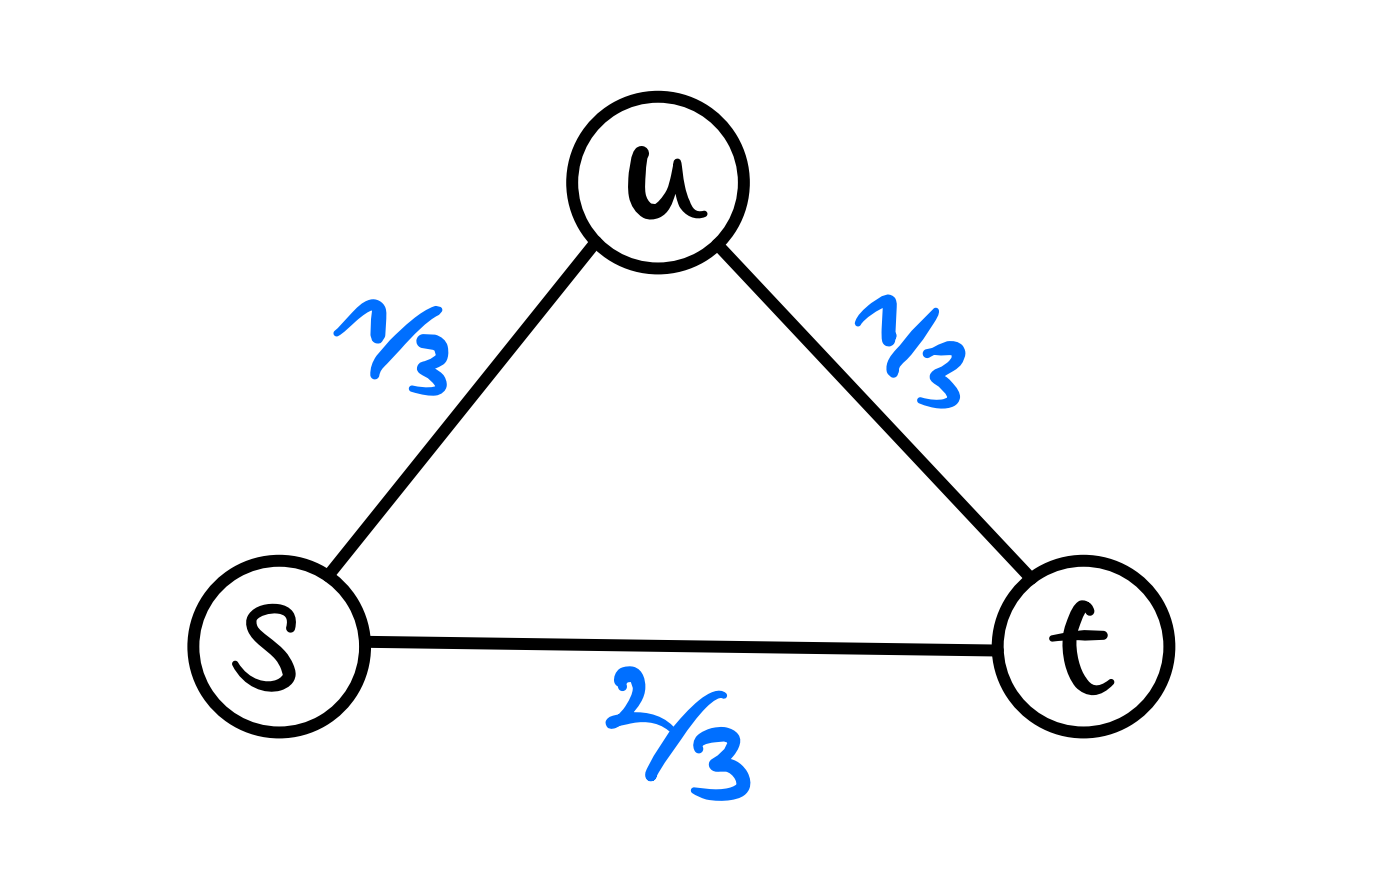
\includegraphics[width=\textwidth]{notes/figures/electrical_flows.png}
    \caption{Example of an electrical flow (shown in blue) with voltages \begin{align*}
        \vx(s) = 0,\quad \vx(u) = 1,\quad \vx(t) = 2
    \end{align*} and unit resistances, routing demands \begin{align*}
        \vd(s) = -1,\quad \vd(u) = 0,\quad \vd(t) = 1.
    \end{align*}}
\end{marginfigure}

To keep track of the direction of flow on each edge, we assign an arbitrary direction to each edge (we ``orient'' $G$) and only consider non-negative flows, $\vf \in \R_{\geq 0}^{|\sE|}$. Clearly, for any previously feasible flow, we can assign directions in such a way that the flow remains feasible.

\section{The Laplacian Matrix}

\begin{defn}[Adjacency matrix]\index{adjacency matrix}
The \emph{adjacency matrix} of a graph $G$, $\Tilde{\mA} \in \R^{|\sV|\times|\sV|}$, is defined as,\footnote{By $\mA$ we will later denote the weighted adjacency matrix.} \begin{align}
    \Tilde{\mA}(u, v) \defeq \begin{cases}
        1 & \text{if $u \sim v$} \\
        0 & \text{otherwise}.
    \end{cases}
\end{align}
\end{defn}
\begin{defn}[Incidence matrix]\index{incidence matrix}
The \emph{incidence matrix} of an oriented graph $G$, $\mB \in \R^{|\sV|\times|\sE|}$, is defined as, \begin{align}
    \mB(v, e) \defeq \begin{cases}
        1 & \text{if $e = (u,v)$ for some $u \in \sV$} \\
        -1 & \text{if $e = (v,u)$ for some $u \in \sV$} \\
        0 & \text{otherwise}.
    \end{cases}
\end{align}
\end{defn} Each column of $\mB$ only has two non-zero entries and sums to one.
\begin{marginfigure}
    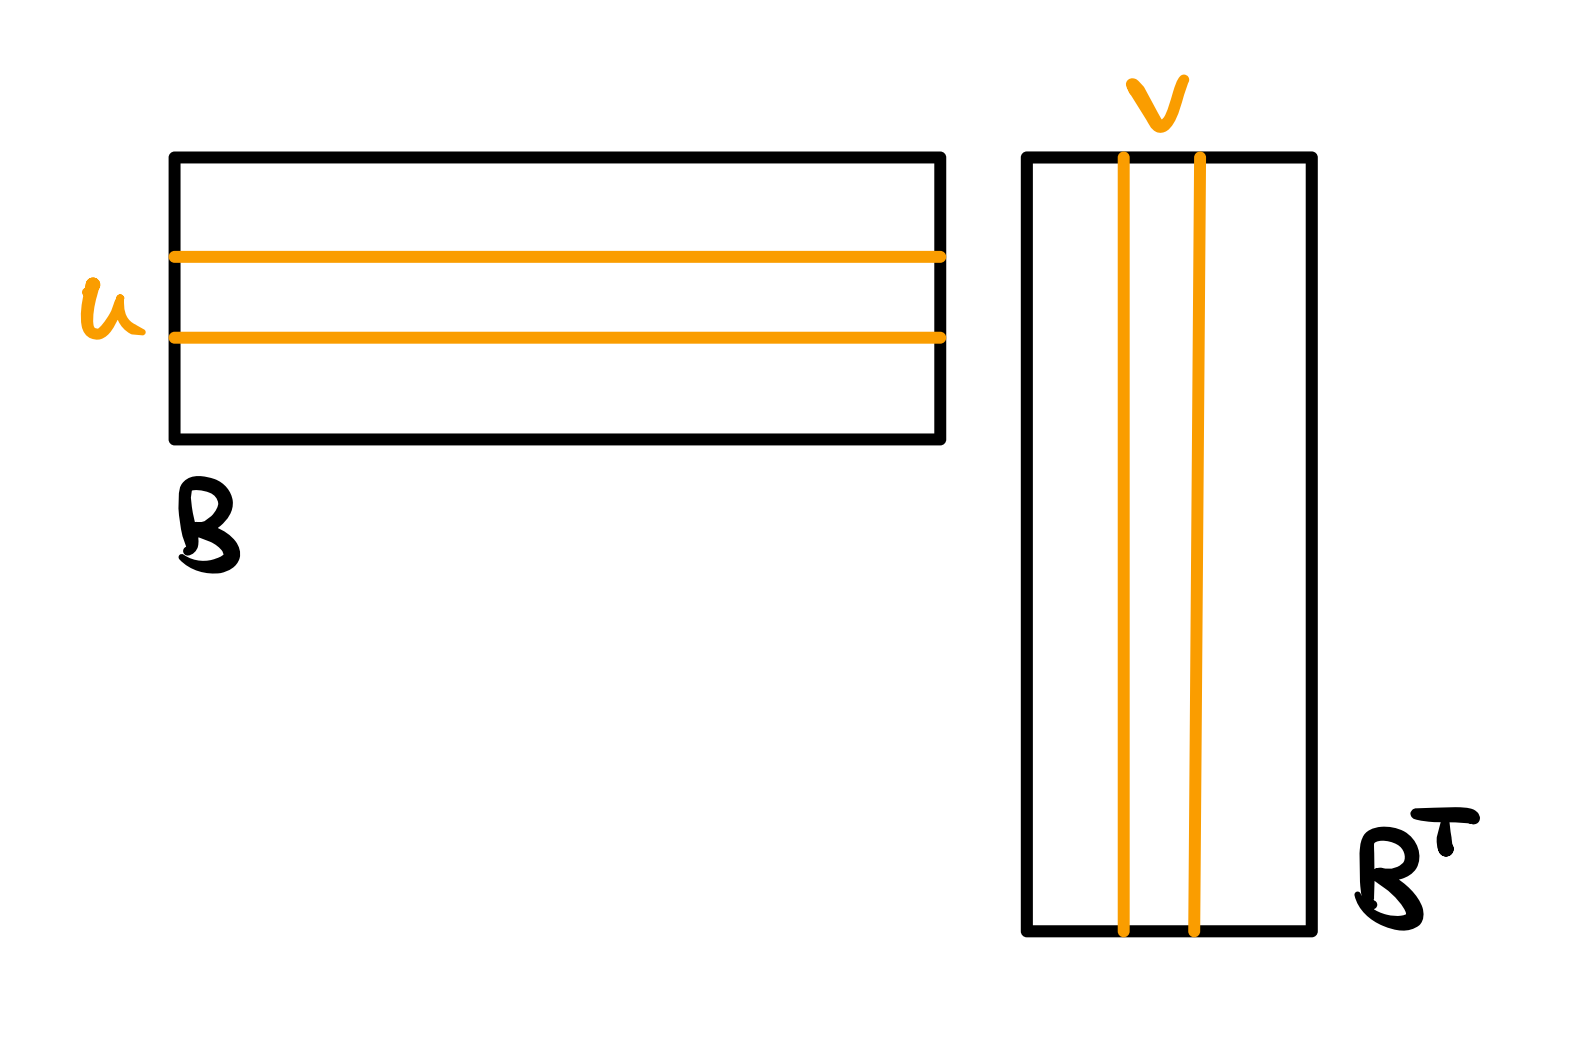
\includegraphics[width=\textwidth]{notes/figures/incidence_matrix.png}
    \caption{Illustration of the matrix product $\mB\trans{\mB}$.}
\end{marginfigure}
\begin{lem}\label{lem:incidence_matrix_product}
$\mB \trans{\mB} = \diag\{\deg(v)\}_{v \in \sV} - \Tilde{\mA}$.
\end{lem}
\begin{proof} The dot product of the rows, corresponding to the same vertex $v$, produces exactly $\deg(v)$. All other dot products between rows corresponding to vertices $u$ and $v$ are $-1$ iff $u \sim v$ and $0$ otherwise.
\end{proof}
We can now also write the net flow constraint\index{net flow constraint}, \begin{align}
    \mB\vf = \vd.
\end{align} We define $\mR \defeq \diag\{\vr(e)\}_{e \in \sE}$ and then have that Ohm's law\index{Ohm's law} can be expressed as, \begin{align}
    \trans{\mB}\vx = \mR\vf, \quad\text{or equivalently,}\quad \mR^{-1}\trans{\mB}\vx = \vf.
\end{align} If the net flow constraint is satisfied, this yields, \begin{align}
    \underbrace{\mB\mR^{-1}\trans{\mB}}_{\text{Laplacian}}\vx = \mB\vf = \vd. \label{eq:ohms_law_and_net_flow_constraint}
\end{align}
\begin{defn}[Laplacian matrix]
The \emph{Laplacian matrix} of an oriented graph $G$, is defined as, \begin{align}
    \mL \defeq \mB\mR^{-1}\trans{\mB} = \mB\mW\trans{\mB} \in \R^{|\sV|\times|\sV|},
\end{align} where $\mW \defeq \mR^{-1}$ is a diagonal matrix of weights\index{weight (of an edge)} $\vw(e) \defeq \frac{1}{\vr(e)}$.
\end{defn}\noindent Intuitively, the weight of an edge can be understood as how ``connected'' the two vertices at its endpoints are. In contrast, the resistance of an edge is smaller when endpoints are well-connected.

We will now learn a little more about Laplacian matrices.
\begin{defn}[Weighted adjacency matrix]\index{weighted adjacency matrix}
The \emph{weighted adjacency matrix} of a graph $G$, $\mA \in \R^{|\sV|\times|\sV|}$, is defined as, \begin{align}
    \mA(u, v) \defeq \begin{cases}
        w(\{u,v\}) & \text{if $u \sim v$} \\
        0 & \text{otherwise}.
    \end{cases}
\end{align}
\end{defn}
\begin{lem}
$\mA$ is symmetric, that is, $\mA = \trans{\mA}$.
\end{lem}
\begin{proof}
This follows immediately from the fact that $G$ is undirected.
\end{proof}
\begin{defn}[Weighted degree]\index{weighted degree}
The \emph{weighted degree} of a vertex $v \in \sV$ is given as, \begin{align}
    \vw(v) \defeq \sum_{\{u,v\} \in \sE} \vw(\{u,v\}).
\end{align} We write $\mD \defeq \diag\{\vw(v)\}_{v \in \sV}$.
\end{defn}

\begin{lem}
$\mL = \mD - \mA$.
\end{lem}
\begin{proof}
The proof is identical to the proof of \cref{lem:incidence_matrix_product}, only that every entry is now weighted, due to the additional factor $\mW$.
\end{proof}

\begin{cor}
$\mL$ is symmetric.
\end{cor}
\begin{proof}
This directly follows from the fact that $\mD$ and $\mA$ are symmetric.\footnote{Diagonal matrices like $\mD$ are trivially symmetric.}
\end{proof}

\begin{lem}
For any $\vx \in \R^{|\sV|}$, we have, \begin{align}
    \trans{\vx}\mL\vx = \sum_{\{u,v\}\in\sE} \vw(\{u, v\})[\vx(u) - \vx(v)]^2 \geq 0.
\end{align}
\end{lem}
\begin{proof}
We have, \begin{align*}
    \trans{\vx}\mL\vx &= \trans{\vx}\mD\vx - \trans{\vx}\mA\vx. \\
    \trans{\vx}\mD\vx &= \sum_{v \in \sV} \vw(v) \vx(v)^2 = \sum_{\{u,v\}\in\sE} \vw(\{u,v\})[\vx(u)^2 + \vx(v)^2]. \\
    \trans{\vx}\mA\vx &= \sum_{v \in \sV} \vx(v) (\mA\vx)(v) \\
    &= \sum_{v \in \sV} \vx(v) \sum_{u \in \sV} \mA(v,u) \vx(u) \\
    &= \sum_{v,u \in \sV} \vw(\{u,v\})\vx(u)\vx(v) \\
    &= 2 \sum_{\{u,v\}\in\sE} \vw(\{u,v\})\vx(u)\vx(v).
\end{align*} Combining the above equalities, we obtain, \begin{align*}
    \trans{\vx}\mL\vx &= \sum_{\{u,v\}\in\sE} \vw(\{u,v\})[\vx(u)^2 + \vx(v)^2] - 2 \sum_{\{u,v\}\in\sE} \vw(\{u,v\})\vx(u)\vx(v) \\
    &= \sum_{\{u,v\}\in\sE} \vw(\{u,v\})[\vx(u) - \vx(v)]^2. \qedhere
\end{align*}
\end{proof}
\begin{cor}
$\mL$ is positive semi-definite.\footnote{By the previous lemma, $\mL$ satisfies the definition of positive semi-definiteness, which we will introduce in the following section.}
\end{cor}

\section{An Optimization Problem}

We have seen that finding voltages $\vx$ or flows $\vf$ is equivalent, we can go from one to the other and back. So let us first focus on how we can find voltages $\vx$.

In \cref{eq:ohms_law_and_net_flow_constraint}, we saw that voltages satisfy $\mL\vx = \vd$, obeying by Ohm's law and satisfying the net flow constraint. A standard approach to reframe the solution to such a system of linear equations as the result of an optimization problem, is to consider the cost function, \begin{align}
    c(\vx) \defeq \frac{1}{2}\trans{\vx}\mL\vx - \trans{\vx}\vd.
\end{align} Observe that $\grad c(\vx) = \mL\vx - \vd \overset{!}{=} 0$ iff $\mL\vx = \vd$. It can also be shown that $c$ is convex, hence, its critical point coincides with its minimizer.\footnote{We will develop tools to show this in the next part. The proof is given in \cref{lem:a1}.} We have therefore recast the problem of finding voltages to the convex optimization, \begin{align}
    \s{\vx} \defeq \argmin_{\vx \in \R^{|\sV|}} c(\vx).
\end{align}

\section{Energy \& Duality}

Let us now look at the same problem through a different lens. Transporting current through a network of resistors requires energy, which is dissipated as heat by the resistor. By \emph{Joule's law}\index{Joule's law}, sending a current $f$ across a resistor with potential drop $x$, spends $f \cdot x$ units of energy per unit time.\footnote{We will think about everything as if happening in one unit of time.} Using Ohm's law, we have, \begin{align}
    f \cdot x = \frac{x^2}{r} = r \cdot f^2.
\end{align} We can therefore write the electrical energy\index{energy} dissipated by routing a flow $\vf$ (or equivalently with voltages $\vx$) as, \begin{align}
    \mathcal{E}(\vf) \defeq \sum_{e \in \sE} \vr(e) \vf(e)^2 = \trans{\vf}\mR\vf = \trans{\vx}\mL\vx \defeq \mathcal{E}(\vx). \margintag{using Ohm's law, $\vf = \mR^{-1}\mB\vx$}
\end{align}

Let us consider the \emph{electrical energy-minimizing flow}\index{electrical energy-minimizing flow}:\footnote{Note that we could instead (and equivalently) characterize the optimization problem using voltages.} \begin{align}
    \s{\vf} \defeq &\argmin_{\substack{\vf \in \R^{|\sE|} \\ \mB\vf = \vd}} \mathcal{E}(\vf). \label{eq:electrical_energy_minimizing_flow}
\end{align} It turns out that $\s{\vf}$ is precisely the electrical flow, that is, $\s{\vf}$ satisfies Ohm's law.\footnote{Proof in \cref{lem:a2}.} This indicates that the two above optimization problems are intimately related: both yield the electrical flow (or equivalently, electrical voltages). In fact, it can be shown that $\mathcal{E}(\s{\vf}) = -c(\s{\vx})$, where we think about maximizing $-c(\vx)$ instead of minimizing $c(\vx)$.\footnote{Proof in \cref{lem:a3}.}. More generally, $\mathcal{E}(\vf) \geq -c(\vx)$ for any flow $\vf$ routing $\vd$ and voltages $\vx$.\footnote{Proof in \cref{lem:a4}.} So, for any $\vx$, the value of $-c(\vx)$ is a lower bound on the minimum energy $\mathcal{E}(\s{\vf})$.

This is an example of a much broader phenomenon known as Lagrangian duality, where we have a minimization problem and a related maximization problem that gives lower bounds on the optimal value of the minimization problem.
	% !TeX root = ../main.tex
% Add the above to each chapter to make compiling the PDF easier in some editors.

\chapter{Linear Algebra}

If a square matrix $\mA \in \R^{n \times n}$ is symmetric\footnote{$\mA$ is symmetric iff $\mA = \trans{\mA}$.}, then $\mA$ has $n$ real \emph{eigenvalues} $\lambda_1, \dots, \lambda_n$ and \emph{eigenvectors} $\vv_1, \dots, \vv_n \in \R^n$ such that $\mA\vv_i = \lambda_i\vv_i$ and the $\vv_i$ are orthogonal\footnote{that is, $\trans{\vv_i}\vv_j = 0$ for $i \neq j$}.\footnote{We prove this in \cref{thm:a5}.}

\begin{defn}[Positive (semi-)definiteness]\index{positive definite matrix}\index{positive semi-definite matrix}\index{indefinite matrix}
Let $\mA \in \R^{n \times n}$ be a symmetric matrix. We say $\mA$ is \begin{enumerate}
    \item \emph{positive definite} iff $\trans{\vx}\mA\vx > 0$ for any $\vx \in \R^n \setminus \{\vZero\}$;
    \item \emph{positive semi-definite} iff $\trans{\vx}\mA\vx \geq 0$ for any $\vx \in \R^n$;
    \item if neither $\mA$ nor $-\mA$ is positive semi-definite, $\mA$ is \emph{indefinite}.
\end{enumerate}
\end{defn}
\begin{thm}\label{thm:psd_eigenvalues}
Let $\mA \in \R^{n \times n}$ be a symmetric matrix. Then, \begin{enumerate}
    \item $\mA$ is positive definite iff all eigenvalues are positive; and
    \item $\mA$ is positive semi-definite iff all eigenvalues are non-negative.
\end{enumerate}
\end{thm}\noindent This theorem is a corollary of the Courant-Fischer theorem, which we will work towards now.

\begin{thm}[Spectral theorem for symmetric matrices]\index{spectral theorem for symmetric matrices} For all symmetric matrices $\mA \in \R^{n \times n}$ there exist \begin{align}
    \mV = \begin{bmatrix}
    \vv_1 & \cdots & \vv_n
    \end{bmatrix} \in \R^{n \times n}, \quad \text{and} \quad \mLambda = \diag\{\lambda_i\}_{i \in [n]} \in \R^{n \times n},
\end{align} where $\lambda_i$ and $\vv_i$ are the eigenvalues and corresponding (normalized) eigenvectors of $\mA$, such that \begin{enumerate}
    \item $\mA = \mV\mLambda\trans{\mV} = \sum_{i=1}^n \lambda_i \vv_i \trans{\vv_i}$; and
    \item $\trans{\mV}\mV = \mI$, i.e., the columns of $\mV$ form an orthonormal basis of $\R^n$.
\end{enumerate}
\end{thm}

\begin{thm}[Courant-Fischer min-max theorem]\index{Courant-Fischer min-max theorem} For symmetric matrices $\mA \in \R^{n \times n}$ with eigenvalues $\lambda_1 \leq \dots \leq \lambda_n$, \begin{align}
    \lambda_i &= \min_{\substack{\text{subspace $\sW \subseteq \R^n$} \\ \dim(\sW) = i}} \max_{\substack{\vx \in \sW \\ \vx \neq \vZero}} \frac{\trans{\vx}\mA\vx}{\trans{\vx}\vx} \label{eq:courant_fischer_1} \\
    &= \max_{\substack{\text{subspace $\sW \subseteq \R^n$} \\ \dim(\sW) = n - i + 1}} \min_{\substack{\vx \in \sW \\ \vx \neq \vZero}} \frac{\trans{\vx}\mA\vx}{\trans{\vx}\vx}.
\end{align}
\end{thm}
\begin{proof}
We show \cref{eq:courant_fischer_1}. The proof of the other equation proceeds analogously. \begin{itemize}
    \item ``$\geq$'': We choose $\sW = \vspan\{\vv_1, \dots, \vv_i\}$ We can write $\vx$ in the basis of eigenvectors, \begin{align*}
        \vx = \sum_{j=1}^i \vc(j) \vv_j
    \end{align*} for some $\vc \in \R^i$. We have, \begin{align*}
        \trans{\vx}\vx = \norm{\vx}_2^2 = \sum_{j=1}^i \sum_{k=1}^i \vc(j) \vc(k) \trans{\vv_j}\vv_k = \sum_{j=1}^i \vc(j)^2, \margintag{using that $\trans{\vv_j}\vv_k = 0$ if $j \neq k$ and $\trans{\vv_j}\vv_k = 1$ otherwise}
    \end{align*} and, \begin{align*}
        \trans{\vx}\mA\vx = \trans{\vx}\mV\mLambda\trans{\mV}\vx &= \trans{(\trans{\mV}\vx)}\mLambda(\underbrace{\trans{\mV}\vx}_{\vc}) \\ &= \trans{\vc}\mLambda\vc = \sum_{j=1}^i \lambda_j \vc(j)^2 \leq \lambda_i \sum_{j=1}^i \vc(j)^2.
    \end{align*} Altogether, \begin{align*}
        \frac{\trans{\vx}\mA\vx}{\trans{\vx}\vx} \leq \lambda_i.
    \end{align*}
    
    \item ``$\leq$'': Consider any subspace $\sW \subseteq \R^n$ with $\dim(\sW) = i$ and fix the subspace $\sT \defeq \vspan\{\vv_i, \dots, \vv_n\}$ with $\dim(\sT) = n - i + 1$. We have that $\dim(\sW \cap \sT) = \dim(\sW) + \dim(\sT) - \dim(\sW \cup \sT)$ and $\dim(\sW \cup \sT) \leq \dim(\R^n) = n$, so, $\dim(\sW \cap \sT) \geq 1$. Therefore, \begin{align*}
        \max_{\substack{\vx \in \sW \\ \vx \neq \vZero}} \frac{\trans{\vx}\mA\vx}{\trans{\vx}\vx} &\geq \max_{\substack{\vx \in \sW \cap \sT \\ \vx \neq \vZero}} \frac{\trans{\vx}\mA\vx}{\trans{\vx}\vx} \\
        &\geq \min_{\substack{\text{subspace $\sV \subseteq \sT$} \\ \dim(\sV) = 1}} \max_{\substack{\vx \in \sV \\ \vx \neq \vZero}} \frac{\trans{\vx}\mA\vx}{\trans{\vx}\vx}.
    \end{align*} For the last inequality note that $\sV$ can be chosen as $\sW \cap \sT$.
    
     We choose $\sV \defeq \vspan\{\vv_i\}$. For some $c \in \R$, we can write $\vx = c\vv_i$. Similarly to the previous part, we obtain, \begin{align*}
         \frac{\trans{\vx}\mA\vx}{\trans{\vx}\vx} = \frac{\lambda_i c^2}{c^2} = \lambda_i. &\qedhere
     \end{align*}
\end{itemize}
\end{proof}

\begin{proof}[Proof of \cref{thm:psd_eigenvalues}] Using Courant-Fischer, we have for the smallest eigenvalue $\lambda_1$ of $\mA$, \begin{align*}
    \lambda_1 = \min_{\substack{\vx \in \R^n \\ \vx \neq \vZero}} \frac{\trans{\vx}\mA\vx}{\trans{\vx}\vx}.
\end{align*} Thus, if $\lambda_{\min}$ is positive, then $\trans{\vx}\mA\vx > 0$ for all $\vx \in \R^n \setminus \{\vZero\}$. In contrast, if for any such $\vx$, $\trans{\vx}\mA\vx > 0$, then $\lambda_1$ must be positive. The proof of positive semi-definiteness is analogous.
\end{proof}

\section{Matrix Norms}

\begin{defn}[Matrix norm]\index{matrix norm} Given a matrix $\mA \in \R^{n \times n}$ and norms $\norm{\cdot}_\alpha$ and $\norm{\cdot}_\beta$ on $\R^n$, the \emph{(induced) norm} of $\mA$ is defined as,\footnote{If you think of $\mA$ as a linear map, you can think of $\norm{\cdot}_\alpha$ as a norm of the input space and $\norm{\cdot}_\beta$ as a norm of the output space.} \begin{align}
    \norm{\mA}_{\alpha\to\beta} \defeq \sup_{\substack{\vx \in \R^n \\ \vx \neq \vZero}} \frac{\norm{\mA\vx}_\beta}{\norm{\vx}_\alpha}.
\end{align} We write $\norm{\mA}_\alpha \defeq \norm{\mA}_{\alpha\to\alpha}$.
\end{defn}

\begin{lem} For a symmetric matrix $\mA \in \R^{n \times n}$, \begin{align}
    \norm{\mA}_2 = \max\{|\lambda_{\min}(\mA)|, |\lambda_{\max}(\mA)|\}.
\end{align} $\norm{\mA}_2$ is called the \emph{spectral norm}\index{spectral norm} of $\mA$.
\end{lem}
\begin{proof}
We have, \begin{align*}
    \norm{\mA}_2^2 &= \sup_{\substack{\vx \in \R^n \\ \vx \neq \vZero}} \frac{\trans{\vx}\trans{\mA}\mA\vx}{\trans{\vx}\vx} \\
    &= \sup_{\substack{\vx \in \R^n \\ \vx \neq \vZero}} \frac{\trans{\vx}\mA^2\vx}{\trans{\vx}\vx} \margintag{using that $\mA$ is symmetric, $\trans{\mA} = \mA$} \\
    &= \sup_{\substack{\vx \in \R^n \\ \vx \neq \vZero}} \frac{\trans{\vx}\mV\mLambda^2\trans{\mV}\vx}{\trans{\vx}\vx} \margintag{using that $\mV$ is orthogonal, $\trans{\mV} = \mV^{-1}$} \\
    &= \sup_{\substack{\vx \in \R^n \\ \vx \neq \vZero}} \frac{\trans{\trans{\mV}\vx}\mLambda^2(\trans{\mV}\vx)}{\trans{\trans{\mV}\vx}(\trans{\mV}\vx)} \\
    &= \sup_{\substack{\vy \in \R^n \\ \vy \neq \vZero}} \frac{\trans{\vy}\mLambda^2\vy}{\trans{\vy}\vy} = \norm{\mLambda}_2^2. \margintag{using that the columns of $\mV$ form a basis of $\R^n$, set $\vy \defeq \trans{\mV}\vx$}
\end{align*} Finally, \begin{align*}
    \norm{\mLambda}_2^2 = \sup_{\substack{\vx \in \R^n \\ \vx \neq \vZero}} \frac{\trans{\vx}\mLambda^2\vx}{\trans{\vx}\vx} = \sup_{\substack{\vx \in \R^n \\ \vx \neq \vZero}} \frac{\sum_{i=1}^n \lambda_i^2 \vx(i)^2}{\sum_{i=1}^n \vx(i)^2} = \max_{i \in [n]} \lambda_i^2. &\qedhere
\end{align*}
\end{proof}

\section{Loewner Order}
% also cover "on graphs"

\section{Pseudo-inverses}

\section{Cholesky Decomposition}
	% !TeX root = ../main.tex
% Add the above to each chapter to make compiling the PDF easier in some editors.

\chapter{Probability}

\section{Random Walks}

In this section, we study random walks on undirected weighted graphs $G = (\sV, \sE, \vw)$ with self-loops. A \emph{random walk}\index{random walk} visits a random sequence of vertices $X_1, X_2, \dots$, where \begin{align}
    \Pr{X_{t+1} = v \mid X_t = u} = \frac{\vw(\{v, u\})}{\vd(u)}
\end{align} and $\vd(u)$ is the weighted degree of vertex $u$, as we have defined previously.

\begin{rmk}
The random walks considered here satisfy the \emph{Markov property}\index{Markov property}, that is, \begin{align}
    X_{t+1} \perp X_1, \dots, X_{t-1} \mid X_t.\safefootnote{So you can think of these random walks as Markov chains.}
\end{align} Moreover, we restrict our attention to time-homogeneous random walks, that is, the transition probabilities remain constant over time.
\end{rmk}

We can therefore model the update of a single round using the linear map $\mW \in \R^{|\sV|\times|\sV|}$ (called \emph{transition matrix}\index{transition matrix}), \begin{align}
    \mW \defeq \begin{bmatrix}
    \frac{\vw(\{1,1\})}{\vd(1)} & \cdots & \frac{\vw(\{n, 1\})}{\vd(n)} \\
    \vdots & \ddots & \vdots \\
    \frac{\vw(\{1,n\})}{\vd(1)} & \cdots & \frac{\vw(\{n, n\})}{\vd(n)} \\
    \end{bmatrix} = \mA\inv{\mD}.
\end{align}

A probability distribution over vertices is a vector $\vp \in \R^{|\sV|}$ such that $\trans{\vOne}\vp = 1$ and $\vp \geq \vZero$. If our initial distribution is $\vp_0$, we have, \begin{align}
    \vp_t = \mW^t\vp_0.
\end{align}

\begin{defn}[Stationary distribution] A distribution $\vpi \in \R^{|\sV|}$ is \emph{stationary}\index{stationary distribution} iff $\vpi = \mW\vpi$.
\end{defn}
\begin{lem}
Every graph has the stationary distribution $\vpi \defeq \frac{\vd}{\trans{\vOne}\vd}$.
\end{lem}\begin{proof} First, $\pi$ is a distribution as, \begin{align*}
    \trans{\vOne}\vpi = \frac{\trans{\vOne}\vd}{\trans{\vOne}\vd}
\end{align*} and clearly $\vpi \geq \vZero$. We have, \begin{align*}
    \mW\vpi = \frac{1}{\trans{\vOne}\vd}\mA\inv{\mD}\vd = \frac{1}{\trans{\vOne}\vd}\mA\vOne = \frac{\vd}{\trans{\vOne}\vd} = \vpi. &\qedhere
\end{align*}
\end{proof}
\begin{rmk}
When the graph is connected, this is the unique stationary distribution.\footnote{In the context of Markov chains, irreducibility is sufficient for a unique stationary condition and equivalent to the transition graph being connected.}
\end{rmk}

\subsection{Lazy Random Walk}

\begin{marginfigure}
\centering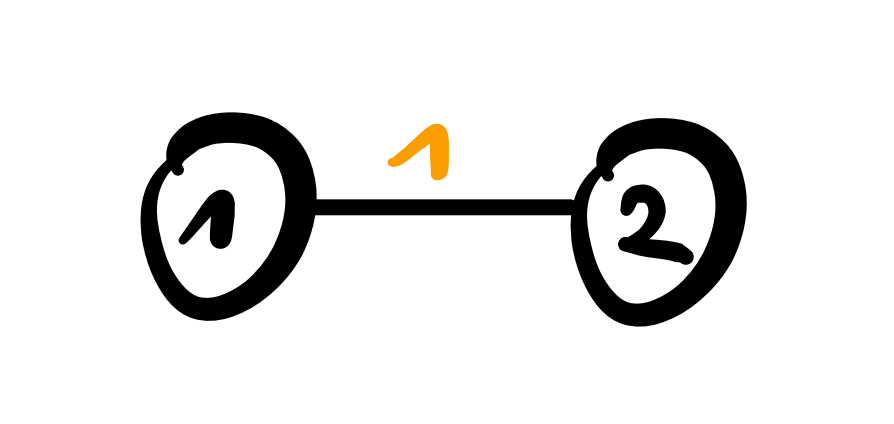
\includegraphics[width=3cm]{notes/figures/not_aperiodic.png}
\caption{Consider the initial distribution $\vp_0(1) = 1, \vp_0(2) = 0$. Clearly, the random walk will forever oscillate between the two states.}\label{fig:not_aperiodic}
\end{marginfigure}

We would also like to have that we converge to this stationary distribution regardless of the initial distribution $\vp_0$, but this is not true for general graphs, as is shown in \cref{fig:not_aperiodic}. A sufficient condition for convergence to the stationary distribution is, however, that all vertices have self-loops.\footnote{It is easy to check that this ensures that the Markov chain is aperiodic, which together with irreducibility implies convergence to the unique stationary distribution.}

Given the random walk $\mW$, the associated \emph{lazy random walk}\index{lazy random walk} is given by, \begin{align*}
    \Tilde{\mW} \defeq \frac{1}{2}\mI + \frac{1}{2}\mW,
\end{align*} that is, we add self-loops to each vertex with weight $\nicefrac{1}{2}$ and halve all other weights. Observe that this does not change the stationary distribution of the random walk. This ensures that the following holds.

\begin{thm}[Convergence of lazy random walk]\label{thm:convergence_of_lazy_random_walk}
For a connected graph, the lazy random walk converges to its unique stationary distribution irrespectively of the initial distribution $\vp_0$, \begin{align}
    \lim_{t\to\infty} \Tilde{\mW}^t\vp_0 = \Tilde{\vpi} = \vpi.
\end{align}
\end{thm}

To prove this theorem, let us first understand the transition matrix in terms of the graph Laplacian.

\begin{lem}
When $\nu_1, \dots, \nu_n$ are the eigenvalues and $\vpsi_1, \dots, \vpsi_n$ the corresponding eigenvectors of the normalized Laplacian matrix $\mN$, then $\Tilde{\mW}$ has eigenvalues $1 - \nicefrac{\nu_i}{2}$ and (not necessarily orthogonal) eigenvectors $\mD^{\nicefrac{1}{2}}\vpsi_i$.
\end{lem}\begin{proof} Let us first express the transition matrix of the original random walk in terms of the normalized graph Laplacian, \begin{align}
    \mW = \mA\inv{\mD} &= \mD^{\nicefrac{1}{2}}(\mD^{-\nicefrac{1}{2}}\mA\mD^{-\nicefrac{1}{2}})\mD^{-\nicefrac{1}{2}} \nonumber\\
    &= \mI + \mD^{\nicefrac{1}{2}}\underbrace{(\mD^{-\nicefrac{1}{2}}\mA\mD^{-\nicefrac{1}{2}} - \mI)}_{-\mN}\mD^{-\nicefrac{1}{2}} \nonumber\\
    &= \mI - \mD^{\nicefrac{1}{2}}\mN\mD^{-\nicefrac{1}{2}} \\
    &= \mD^{\nicefrac{1}{2}}(\mI - \mN)\mD^{-\nicefrac{1}{2}}. \nonumber
\end{align} By \cref{lem:a7}, $\mD^{\nicefrac{1}{2}}(\mI - \mN)\mD^{-\nicefrac{1}{2}}$ and $\mI - \mN$ have the same eigenvalues, namely $1 - \nu_i$. We also have, \begin{align}
    \Tilde{\mW} = \frac{1}{2}\mI + \frac{1}{2}(\mI - \mD^{\nicefrac{1}{2}}\mN\mD^{-\nicefrac{1}{2}}) = \mI - \frac{1}{2}\mD^{\nicefrac{1}{2}}\mN\mD^{-\nicefrac{1}{2}},
\end{align} implying that the eigenvalues of $\Tilde{\mW}$ are $1 - \nicefrac{\nu_i}{2}$. Finally, we have, \begin{align*}
    \Tilde{\mW}\mD^{\nicefrac{1}{2}}\vpsi_i &= (\mI - \frac{1}{2}\mD^{\nicefrac{1}{2}}\mN\mD^{-\nicefrac{1}{2}})\mD^{\nicefrac{1}{2}}\vpsi_i \\
    &= \mD^{\nicefrac{1}{2}}\vpsi_i - \frac{1}{2}\mD^{\nicefrac{1}{2}}\mN\vpsi_i \\
    &= \mD^{\nicefrac{1}{2}}\vpsi_i - \frac{\nu_i}{2}\mD^{\nicefrac{1}{2}}\vpsi_i \margintag{using that $\vpsi_i$ is an eigenvector of $\mN$ with corresponding eigenvalue $\nu_i$} \\
    &= \parentheses*{1 - \frac{\nu_i}{2}}\mD^{\nicefrac{1}{2}}\vpsi_i. \qedhere
\end{align*}
\end{proof}

\begin{proof}[Proof of \cref{thm:convergence_of_lazy_random_walk}]
TBD
\end{proof}

\begin{thm}[Convergence rate of lazy random walk]
For any unweighted connected graph $G$, we have that at time step $t$,\footnote{We will later see that $\nu_2$ is an indicator of the ``connectedness'' of $G$.} \begin{align}
    \norm{\vp_t - \vpi}_\infty \leq e^{-\nicefrac{\nu_2 t}{2}}\sqrt{n}.
\end{align}
\end{thm}
\begin{proof}
TBD
\end{proof}

\subsection{Hitting Time}

\begin{defn}[Hitting time] The \emph{hitting time}\index{hitting time}, \begin{align}
    H_{a,s} \defeq \min\{t \geq 1 \mid X_t = s, X_0 = a\},
\end{align} is the number of steps to reach $s$ starting from $a$. We have, \begin{align}
    \vh_s(a) \defeq \E{H_{a,s}} = 1 + \sum_{b \sim a} \frac{\vw(\{a,b\})}{\vd(a)} \vh_s(b). \label{eq:expected_hitting_time}
\end{align}
\end{defn}

\begin{lem}
If $\elx$ is a solution to $\mL\elx = \vd - \norm{\vd}_1 \vOne_s$,\footnote{We use $\vOne_s$ as a shorthand notation for $\vOne_{\{s\}}$.} then \begin{align}
    \vh_s = \elx - \elx(s)\vOne.
\end{align}
\end{lem}
\begin{proof}
For any $a \neq s$, we can equivalently write \cref{eq:expected_hitting_time} as, \begin{align*}
    \trans{\vOne_a}\vh_s = 1 + \trans{(\mW \vOne_a)}\vh_s \iff \trans{\vOne_a}(\mI - \trans{\mW})\vh_s = 1.
\end{align*} This yields a linear system of $n-1$ equations, \begin{align}
    \vOne - \alpha \vOne_s = (\mI - \underbrace{\trans{\mW}}_{\inv{\mD}\mA})\vh_s,
\end{align} where $\alpha$ is due to the remaining degree of freedom, as the entry corresponding to $s$ is not fixed. Multiplying from the left with $\mD$, we obtain, \begin{align*}
    \vd - \alpha \vd(s) \vOne_s = (\mD - \mA)\vh_s = \mL\vh_s.
\end{align*} Recall that $\ker{\mL} = \vspan\{\vOne\}$, and hence, for $\vh$ to exist, we must choose $\alpha$ such that $\vd - \alpha \vd(s) \vOne_s \perp \vOne$. We have, \begin{align*}
    \trans{\vOne}(\vd - \alpha \vd(s) \vOne_s) = \norm{\vd}_1 - \alpha \vd(s) \overset{!}{=} 0 \iff \alpha = \frac{\norm{\vd}_1}{\vd(s)}.
\end{align*} Finally, note that the solution $\elx$ to $\mL\elx = \vd - \norm{\vd}_1 \vOne_s$ is not unique. Given that $\vh_s$ is one solution, we have that any $\elx = \vh_s + c\vOne$ for $c \in \R$ is also a solution.\footnote{This follows directly from the fact that $\ker{\mL} = \vspan\{\vOne\}$.} Yet, we know that $\vh_s(s) = 0$, implying that $\vh_s = \elx - \elx(s)\vOne$.
\end{proof}

\subsection{Commute Time}

\begin{marginfigure}
TBD
% \centering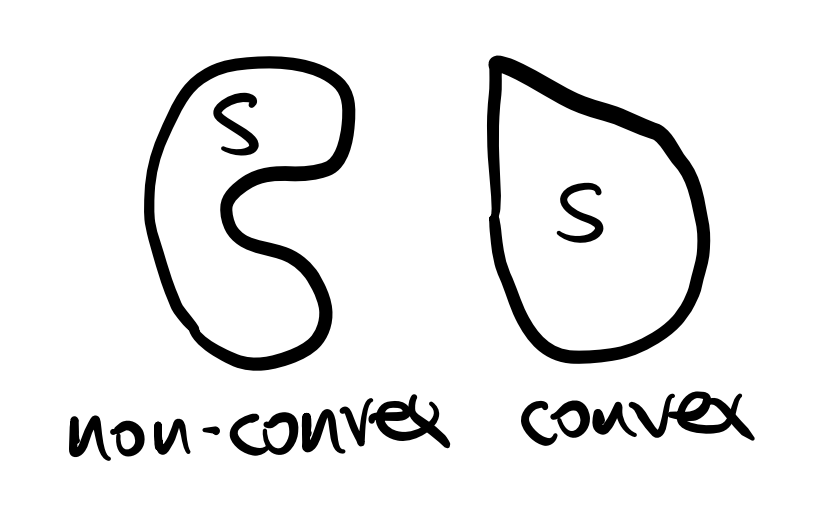
\includegraphics[width=4cm]{notes/figures/convex_set.png}
\caption{Example where hitting times are not symmetric.}
\end{marginfigure}
An issue with hitting times is that they do not need to be symmetric. This motivates the consideration of commute times, which correspond to the number of steps it takes to reach $b$ from $a$ and return to $a$.

\begin{defn}[Commute time] The \emph{commute time}\index{commute time} between $a$ and $b$ is defined as, \begin{align}
    C_{a,b} \defeq H_{a,b} + H_{b,a}.
\end{align}
\end{defn}
\begin{rmk}
By definition, commute times are symmetric.
\end{rmk}

\begin{lem}
If $\elx$ is a solution to $\mL\elx = \norm{\vd}_1 (\vOne_a - \vOne_b)$, then \begin{align}
    \E{C_{a,b}} = \trans{(\vOne_a - \vOne_b)}\elx = \elx(a) - \elx(b).
\end{align}
\end{lem} The $\elx$ can be interpreted as electrical voltages inducing flow that routes $\norm{\vd}_1$ units from $a$ to $b$.
\begin{proof}
We write $\vb_v \defeq \vd - \norm{\vd}_1 \vOne_v$ and let $\mL\ey = \vb_b$ and $\mL\ez = \vb_a$. Then, \begin{align*}
    \E{C_{a,b}} &= \vh_b(a) + \vh_a(b) \\
    &= \ey(a) - \ey(b) + \ez(b) - \ez(a) \\
    &= \trans{(\vOne_a - \vOne_b)}(\ey - \ez).
\end{align*} Observe that $\elx \defeq \ey - \ez$ solves $\mL\elx = \vb_b - \vb_a = \norm{\vd}_1 (\vOne_a - \vOne_b)$.
\end{proof}

We will see in \cref{cha:effective_resistance} that the expected commute time is intimately related to the electrical energy required to route flow from $a$ to $b$, also called the effective resistance between $a$ and $b$.

\section{Concentration}

\begin{thm}[Markov's inequality]\index{Markov's inequality}
For any random variable $X \geq 0$ and $t > 0$, \begin{align}
    \Pr{X \geq t} \leq \frac{\E{X}}{t}.
\end{align}
\end{thm}
\begin{proof} We have, \begin{align*}
    \E{X} = \int_0^\infty x f(x) \,dx \geq \int_t^\infty x f(x) \, dx \geq t \int_t^\infty f(x) \,dx = t \Pr{X \geq t},
\end{align*} where $f$ is the probability density function of $X$.
\end{proof}

\begin{thm}[Jensen's inequality]\index{Jensen's inequality}
For a random variable $X$, if $f$ is convex, then $\E{f(X)} \geq f(\E{X})$.\footnote{Proof of the finite form in \cref{thm:a8}.}
\end{thm}
\begin{marginfigure}
TBD
% \centering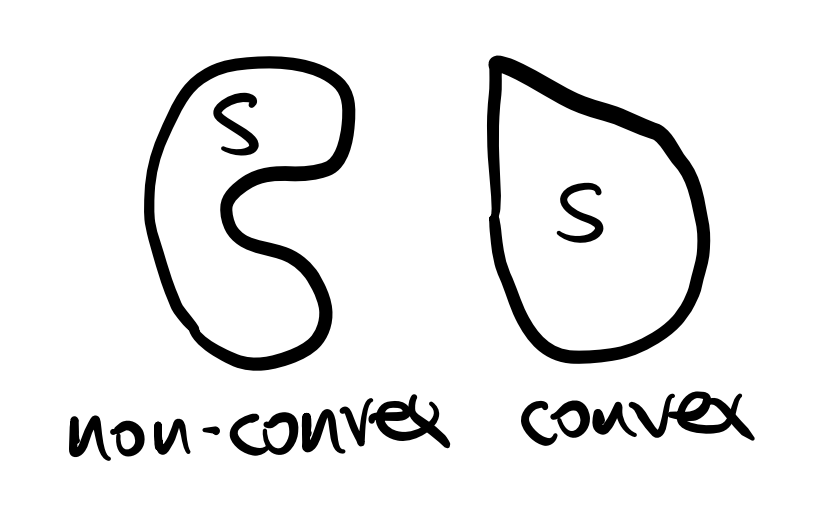
\includegraphics[width=4cm]{notes/figures/convex_set.png}
\caption{Jensen's inequality.}
\end{marginfigure}

\begin{thm}[Bernstein concentration bound]\index{Bernstein concentration bound} Given independent real-valued random variables $X_1, \dots, X_k \in \R$ such that $\E{X_i} = 0$ and $|X_i| \leq R$. Let $X \defeq \sum_i X_i$ and $\sigma^2 \defeq \Var{X} = \sum_i \E{X_i^2}$. Then, for $t > 0$, \begin{align}
    \Pr{|X| \geq t} \leq 2 \exp\parentheses*{\frac{-t^2}{2Rt + 4\sigma^2}}.
\end{align}
\end{thm}
\begin{proof}
TBD
\end{proof}

\begin{thm}[Bernstein matrix concentration bound]\index{Bernstein matrix concentration bound} Suppose $\rX_1, \dots, \rX_k \in \R^{n \times n}$ are independent symmetric matrix-valued random variables satisfying $\E{\rX_i} = \mZero$ and $\norm{\rX_i}_2 \leq R$. Let $\rX \defeq \sum_i \rX_i$ and $\sigma^2 \defeq \Var{\rX} = \sum_i \E{\rX_i^2}$. Then, for $t > 0$, \begin{align}
    \Pr{\norm{\rX}_2 \geq t} \leq 2 n \exp\parentheses*{\frac{-t^2}{2Rt + 4\sigma^2}}.
\end{align}
\end{thm}
\begin{proof}
TBD
\end{proof}

\section{Martingales}

\begin{defn}[Martingale] A \emph{martingale}\index{martingale} is a sequence of random variables $Z_0, \dots, Z_k$ such that \begin{align}
    \E{Z_i \mid Z_0, \dots, Z_{i-1}} = Z_{i-1}.
\end{align} That is, conditional on the outcome of all the previous random variables, the expectation of $Z_i$ equals $Z_{i-1}$.% In particular, $\E{Z_k} = \E{Z_0}$.
\end{defn} Typically, we use martingales to show a statement such as ``$Z_k$ is concentrated around $\E{Z_k}$''.

We can alternatively think of a martingale as the sequence of changes in $Z_i$. Let $X_i \defeq Z_i - Z_{i-1}$. The sequence of $X_i$ is called \emph{martingale difference sequence}\index{martingale difference sequence}. The martingale condition is equivalent to, \begin{align}
    \E{X_i \mid Z_0, \dots, Z_{i-1}} = \E{X_i \mid Z_0, X_1, \dots, X_{i-1}} = 0.
\end{align} We can write, \begin{align}
    Z_k = Z_0 + \sum_{i=1}^k Z_i - Z_{i-1} = Z_0 + \sum_{i=1}^k X_i.
\end{align}
	% !TeX root = ../main.tex
% Add the above to each chapter to make compiling the PDF easier in some editors.

\chapter{Analysis}

In this chapter, we study functions $f: \sS \to \R$ where $\sS \subseteq \R^n$.

\section{First-order Taylor Approximations}

\begin{defn}[Gradient] The \emph{gradient}\index{gradient} of a function $f: \sS \to \R$ at point $\vx \in \sS$ is, \begin{align}
    \grad f(\vx) \defeq \trans{\begin{bmatrix}
        \pdv{f(\vx)}{\vx(1)} & \cdots & \pdv{f(\vx)}{\vx(n)}
    \end{bmatrix}}.
\end{align}
\end{defn}

For a single-variable function $f: \R \to \R$ that is differentiable, we have for any $x, \delta \in \R$, \begin{align*}
    f(x + \delta) = f(x) + \odv{f(x)}{x} + o(|\delta|), \quad \text{where } \lim_{\delta \to 0} \frac{o(|\delta|)}{|\delta|} = 0,
\end{align*} using a first-order Taylor approximation around $x$. We can use a similar approximation when $f$ is a multi-variable function.

\begin{defn}[Fréchet differentiability] A function $f: \sS \to \R$ is \emph{(Fréchet) differentiable}\index{Fréchet differentiability} at $\vx \in \sS$ if there exists $\vg \in \R^n$ such that, \begin{align}
    \lim_{\substack{\vdelta \in \R^n \\ \vdelta \to \vZero}} \frac{|f(\vx + \vdelta) - (f(\vx) + \trans{\vg}\vdelta)|}{\norm{\vdelta}_2} = 0.
\end{align}
\end{defn}\noindent Here, $\vg$ can be understood as a candidate for $\grad f(\vx)$ and $f(\vx) + \trans{\vg}\vdelta$ is a linear approximation of $f$ around $\vx$.

This notion of differentiability is equivalent to, \begin{align}
    f(\vx + \vdelta) = f(\vx) + \trans{\grad f(\vx)}\vdelta + o(\norm{\vdelta}_2),
\end{align} for any $\vx, \vdelta \in \R^n$. This is also called a \emph{first-order expansion}\index{first-order expansion} of $f$.

\begin{defn}[Continuous differentiability] We say that $f : \sS \to \R$ is \emph{continuously differentiable}\index{continuous differentiability} on $\sS$ if it is differentiable and its gradient is continuous on $\sS$.
\end{defn}
\begin{lem} A differentiable and convex function $f$, whose domain $\sS \subseteq \R^n$ is open and convex, is always continuously differentiable.
\end{lem}

\begin{thm}[Taylor's theorem]\index{Taylor's theorem} If $f: \sS \to \R$ is continuously differentiable, then for all $\vx, \vy \in \R^n$, \begin{align}
    f(\vy) = f(\vx) + \trans{\grad f(\vz)}(\vy - \vx),
\end{align} for some $\vz \in [\vx, \vy] \defeq \{\theta\vx + (1-\theta)\vy \mid \theta \in [0,1]\}$.
\end{thm}\begin{marginfigure}
\centering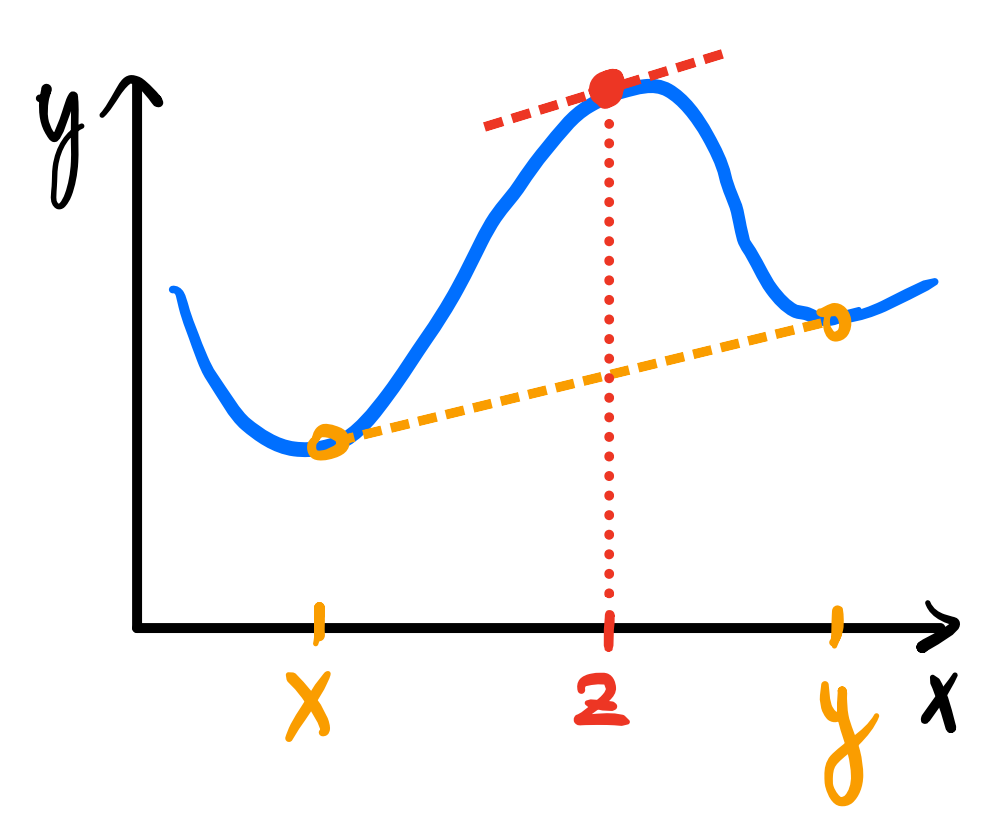
\includegraphics[width=3cm]{notes/figures/taylors_theorem.png}
\caption{Illustration of Taylor's theorem. The affine approximation is shown in orange.}
\end{marginfigure}\noindent Taylor's theorem implies that $f$ can be approximated by the affine function, \begin{align*}
    \vy \to f(\vx) + \trans{\grad f(\vx)}(\vy - \vx),
\end{align*} when $\vy$ is ``close to'' $\vx$.

\section{Directional Derivatives}

\begin{defn}[Directional derivative] Let $f: \sS \to \R$ be differentiable at $\vx \in \R^n$. Given $\vd \in \R^n$, the \emph{directional derivative}\index{directional derivative} of $f$ at $\vx$ in the direction $\vd$ is, \begin{align}
    D f(\vx)[\vd] \defeq \lim_{\lambda \to 0} \frac{f(\vx + \lambda\vd) - f(\vx)}{\lambda}.
\end{align}
\end{defn}

\begin{lem} $D f(\vx)[\vd] = \trans{\grad f(\vx)}\vd$.
\end{lem}
\begin{proof} Using a first-order expansion, we have, \begin{align*}
    f(\vx + \lambda\vd) = f(\vx) + \lambda \trans{\grad f(\vx)}\vd + o(\lambda \norm{\vd}_2).
\end{align*} Dividing by $\lambda$ yields, \begin{align*}
    \frac{f(\vx + \lambda\vd) - f(\vx)}{\lambda} = \trans{\grad f(\vx)}\vd + \underbrace{\frac{o(\lambda\norm{\vd}_2)}{\lambda}}_{\to 0}.
\end{align*} Taking the limit $\lambda \to 0$ gives the desired result.
\end{proof}

\section{Conditions for Optimality}

\begin{defn}[Stationary point] Given a function $f: \sS \to \R$, a point $\vx \in \sS$ where $\grad f(\vx) = 0$ is called a \emph{stationary point}\index{stationary point} of $f$.\footnote{Being a stationary point is not sufficient for optimality. Take for example the point $x \defeq 0$ of $f(x) \defeq x^3$.}
\end{defn}

\begin{lem}
If $\vx \in \sS$ is a local extremum of a differentiable function $f: \sS \to \R$, then $\grad f(\vx) = 0$.\footnote{Here it is important that we have chosen $\sS \subseteq \R^n$ to be open. When $\sS$ is not open, an extremum could be on the boundary of the domain, where the gradient is non-zero.}
\end{lem}
\begin{proof}
    Assume $\vx$ is a local minimum of $f$. Then, for all $\vd \in \R^n$ and for all small enough $\lambda \in R$, we have $f(\vx) \leq f(\vx + \lambda\vd)$, so, \begin{align*}
        0 &\leq f(\vx + \lambda\vd) - f(\vx) \\
        &= \lambda \trans{\grad f(\vx)}\vd + o(\lambda\norm{\vd}_2). \margintag{using a first-order expansion of $f$ around $x$}
    \end{align*} Dividing by $\lambda$ and taking the limit $\lambda \to 0$, we obtain, \begin{align*}
        0 \leq \trans{\grad f(\vx)}\vd + \underbrace{\frac{o(\lambda\norm{\vd}_2)}{\lambda}}_{\to 0} \to \trans{\grad f(\vx)}\vd.
    \end{align*} Take $\vd \defeq - \grad f(\vx)$.\footnote{We can only take this step because we assumed that $\sS$ is open.} Then, \begin{align*}
        0 \leq - \norm{\grad f(\vx)}_2^2,
    \end{align*} so $\grad f(\vx) = 0$.
\end{proof}

\section{Second-order Taylor Approximations}

    \part{Convex Optimization}\label{part2}
    % !TeX root = ../main.tex
% Add the above to each chapter to make compiling the PDF easier in some editors.

\chapter{Convex Geometry}

We want to develop a better understanding of optimization problems. The general form of an \emph{optimization problem}\index{optimization problem} is, \begin{align}
    \min_{\substack{\vx \in \R^n \\ g_1(\vx) \leq b_1 \\ \vdots \\ g_m(\vx) \leq b_m}} f(\vx), \label{eq:optimization_problem}
\end{align} where $f : \R^n \to \R$ and $g_i : \R^n \to \R$.\footnote{It suffices to consider minimization problems. If we want to maximize a function $f$, this is equivalent to minimizing the function $-f$.}

\begin{defn}[Feasible set] We call \begin{align}
    \spa{F} \defeq \{\vx \in \R^n \mid \forall i \in [n]: g_i(\vx) \leq b_i\}
\end{align} the \emph{feasible set}\index{feasible set}. We call \begin{itemize}
    \item $\vx \in \spa{F}$ a \emph{feasible point}\index{feasible point}; and
    \item $\vx \not\in \spa{F}$ an \emph{infeasible point}\index{infeasible point}.
\end{itemize}
\end{defn}
\begin{defn}[Optimal solution] We say that $\s{\vx} \in \R^n$ is \emph{optimal}\index{optimal point} if $\s{\vx} \in \spa{F}$ and $\forall \vx \in \spa{F}: f(\s{\vx}) \leq f(\vx)$.
\end{defn}
\begin{marginfigure}
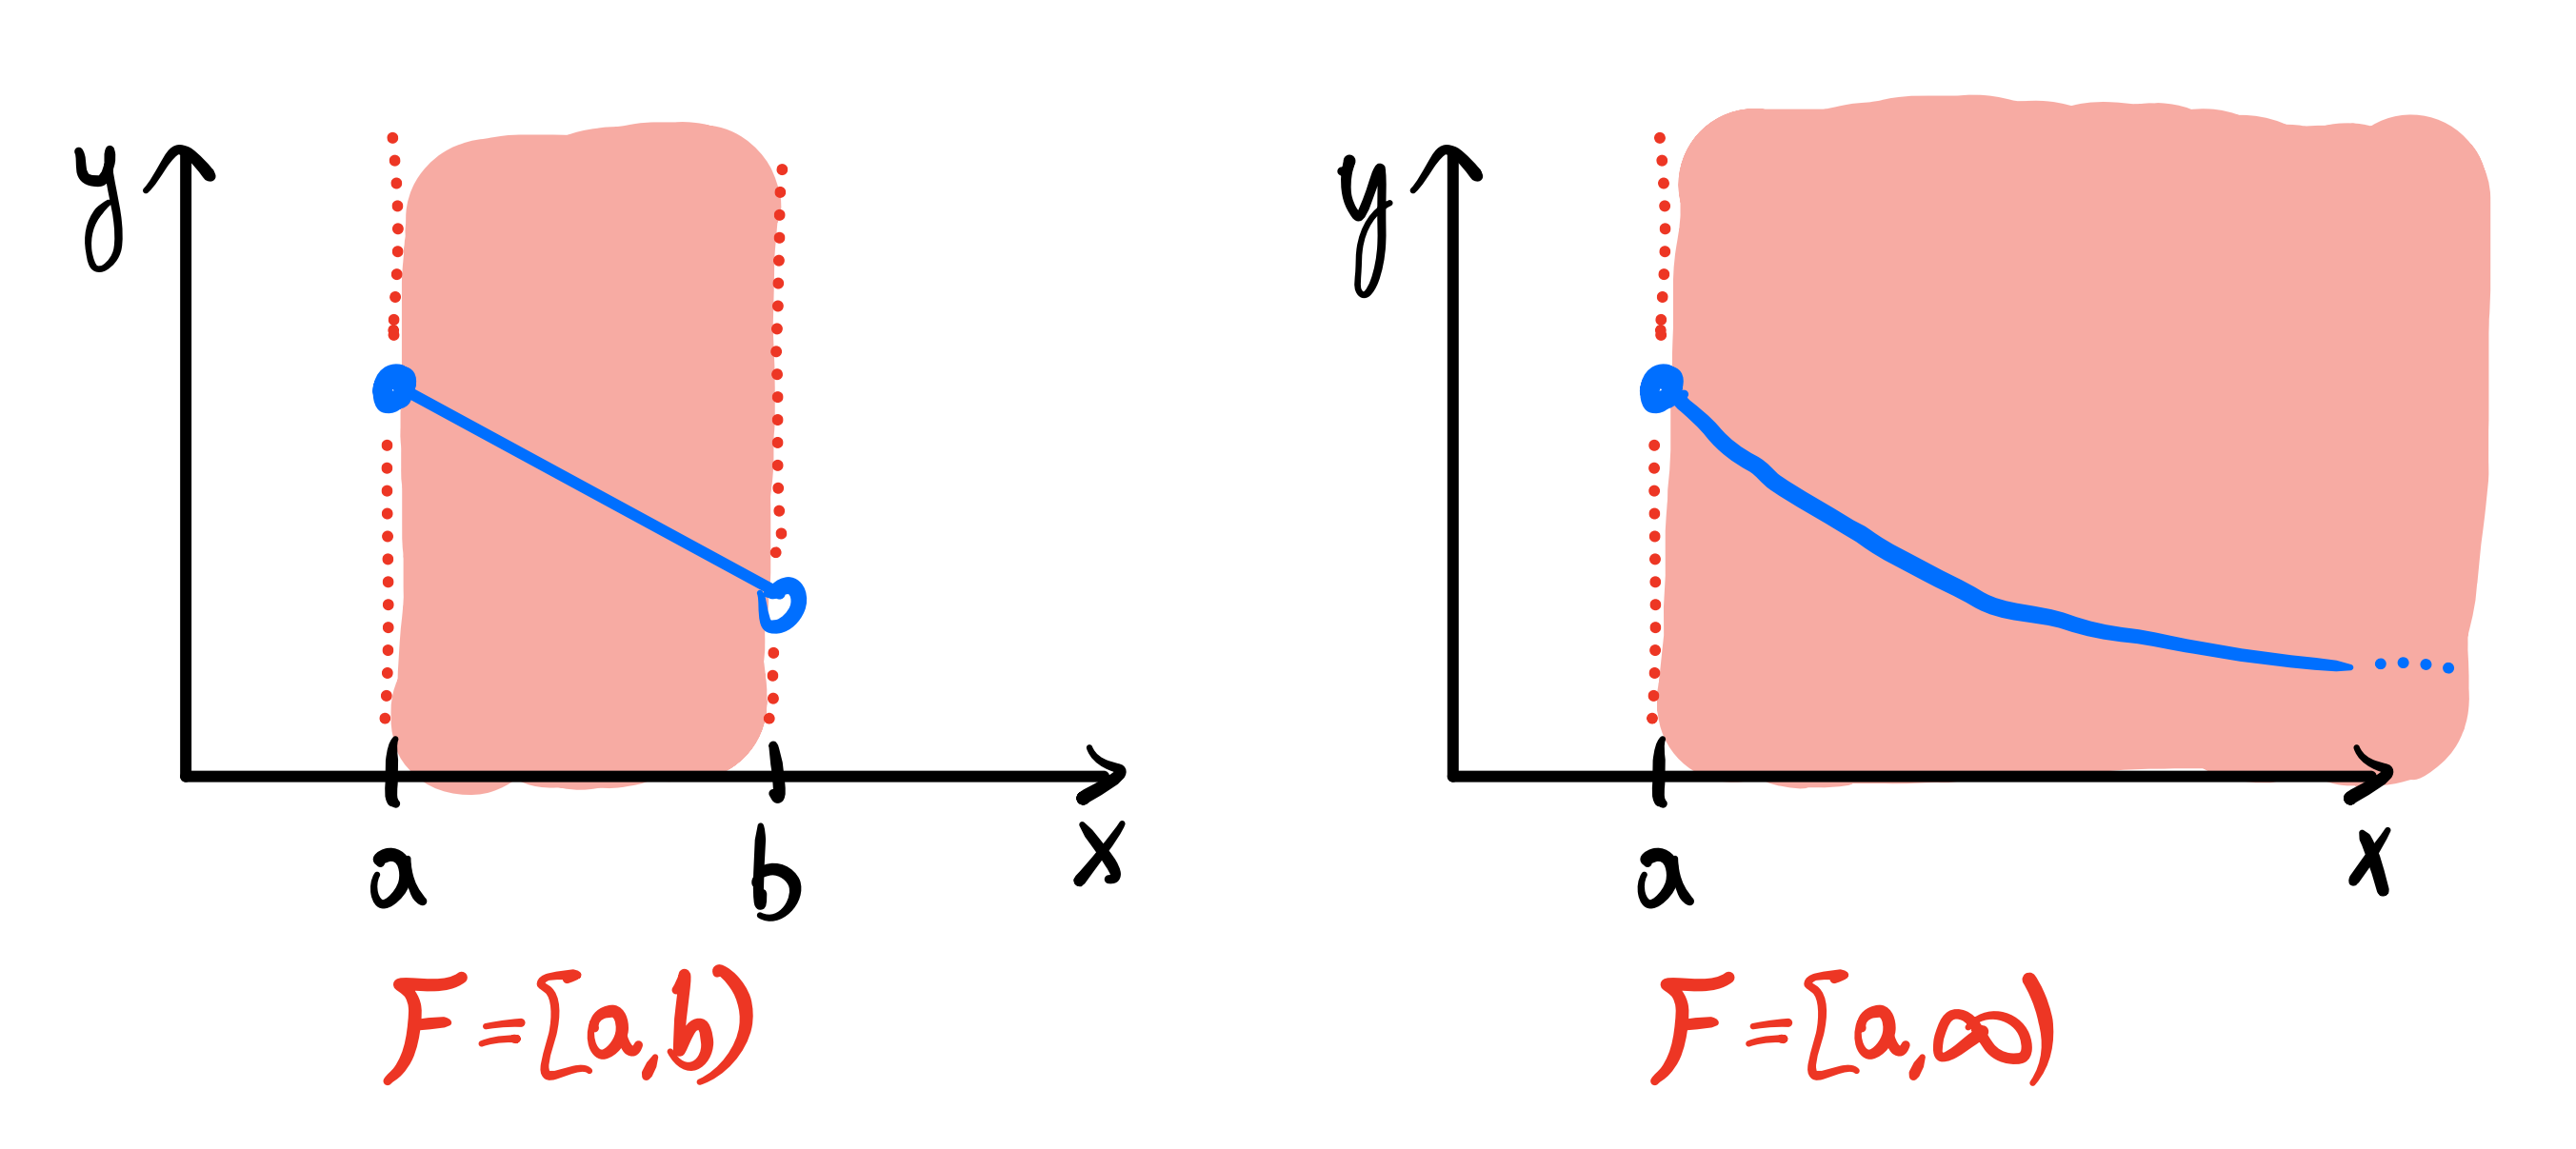
\includegraphics[width=\textwidth]{notes/figures/no_opt.png}
\caption{Examples of optimization problems without an optimal solution.}
\end{marginfigure}

Let us look at a sufficient condition for optimal solutions. \begin{thm}[Extreme value theorem]\index{extreme value theorem}\label{thm:extreme_value_theorem}
Let $f : \R^n \to \R$ be continuous, and let $\spa{F} \subseteq \R^n$ be non-empty, bounded, and closed. Then, $f$ is bounded on $\spa{F}$ and has an optimal solution.
\end{thm}

\section{Convex Sets \& Functions}

\begin{defn}[Convex set] A set $\sS \subseteq \R^n$ is \emph{convex}\index{convex set} iff \begin{align}
    \forall \vx, \vy \in \sS: \forall \theta \in [0,1]: \theta\vx + (1-\theta)\vy \in \sS.
\end{align}
\end{defn}
\begin{marginfigure}
\centering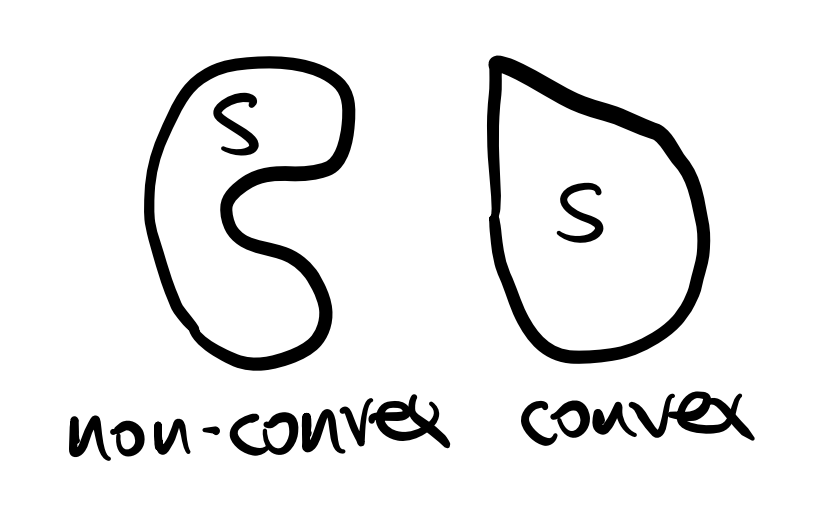
\includegraphics[width=4cm]{notes/figures/convex_set.png}
\caption{Example of a non-convex and a convex set.}
\end{marginfigure}
\begin{defn}[Convex function] For a convex set $\sS \subseteq \R^n$, a function $f : \sS \to \R$ is \emph{convex}\index{convex function} on $\sS$ iff \begin{align}
    \forall \vx, \vy \in \sS: \forall \theta \in [0,1]: f(\theta\vx + (1-\theta)\vy) \leq \theta f(\vx) + (1-\theta) f(\vy).
\end{align} Similarly, we call $f$ \emph{strictly convex}\index{strictly convex function} on $\sS$ iff \begin{align}
    \forall \vx, \vy \in \sS: \forall \theta\in[0,1]: f(\theta\vx + (1-\theta)\vy) < \theta f(\vx) + (1-\theta) f(\vy).
\end{align}
\end{defn}
\begin{marginfigure}
\centering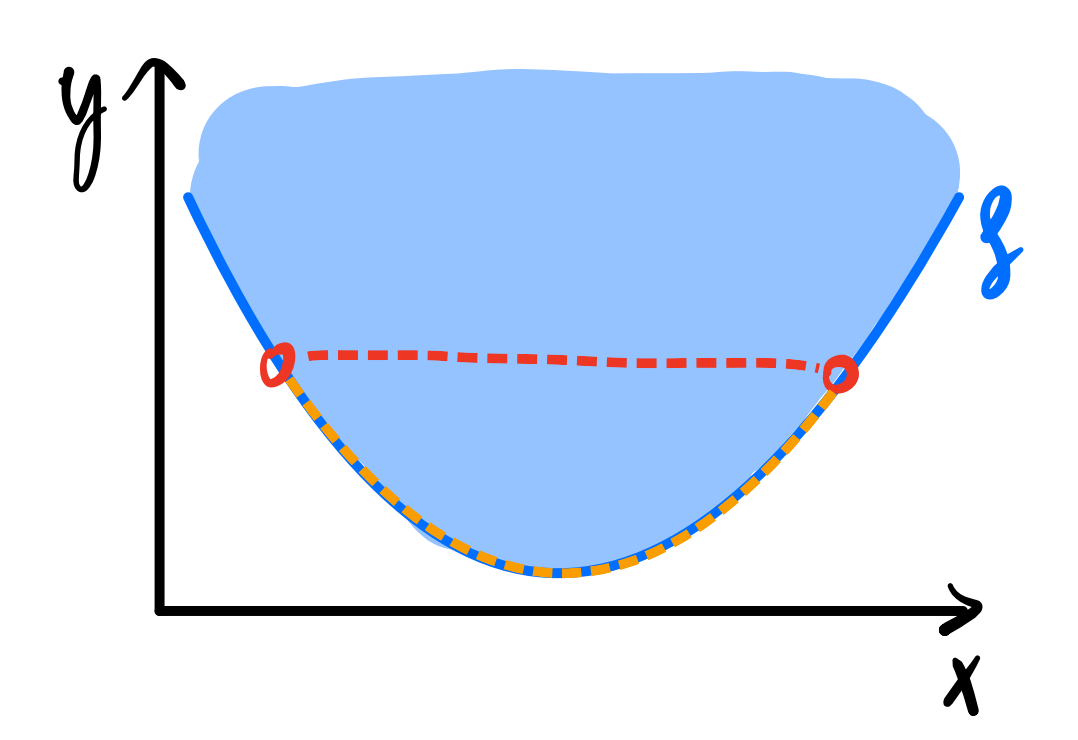
\includegraphics[width=3cm]{notes/figures/convex_function.png}
\caption{Example of a convex function. Any line between two points on $f$, lies ``above'' $f$. The epigraph of $f$ is shown in blue.}
\end{marginfigure}

\begin{rmk}
If the function $f$ is convex on $\sS$, we say that the function $-f$ is \emph{concave}\index{concave function} on $\sS$.
\end{rmk}

\begin{lem} A differentiable and convex function $f$, whose domain $\sS \subseteq \R^n$ is open and convex, is always continuously differentiable.
\end{lem} In the following, we will assume that $\sS \subseteq \R^n$ is open.

\begin{defn}[Epigraph]
The \emph{epigraph}\index{epigraph} of a function $f : \sS \to \R$ is \begin{align}
    \mathrm{epi}(f) \defeq \{(\vx,y) \mid f(\vx) \leq y\} \subseteq \R^{n+1}.
\end{align}
\end{defn}
\begin{exc}\label{exc:convex_iff_epi_convex}
The function $f : \sS \to \R$ is convex iff $\mathrm{epi}(f)$ is convex.
\end{exc}

\begin{defn}[(Sub-)level set] Given a function $f : \sS \to \R$, we call, \begin{align}
    \sS_\alpha(f) &\defeq \{\vx \in \sS \mid f(\vx) \leq \alpha\}, \\
    \sL_\alpha(f) &\defeq \{\vx \in \sS \mid f(\vx) = \alpha\},
\end{align} its \emph{$\alpha$-sub-level set}\index{sub-level set} and \emph{$\alpha$-level set}\index{level set}, respectively.
\end{defn}
\begin{exc}\label{exc:sub_level_set_of_convex_function_convex}
Any $\alpha$-sub-level set of a convex function is convex.\footnote{Note that the other direction does not hold! Take $f(x) \defeq x^3$ as an example. Functions whose sub-level sets are convex are called \emph{quasiconvex}\index{quasiconvex function}.}
\end{exc}

\section{First-order Characterization of Convexity}

\begin{marginfigure}
\centering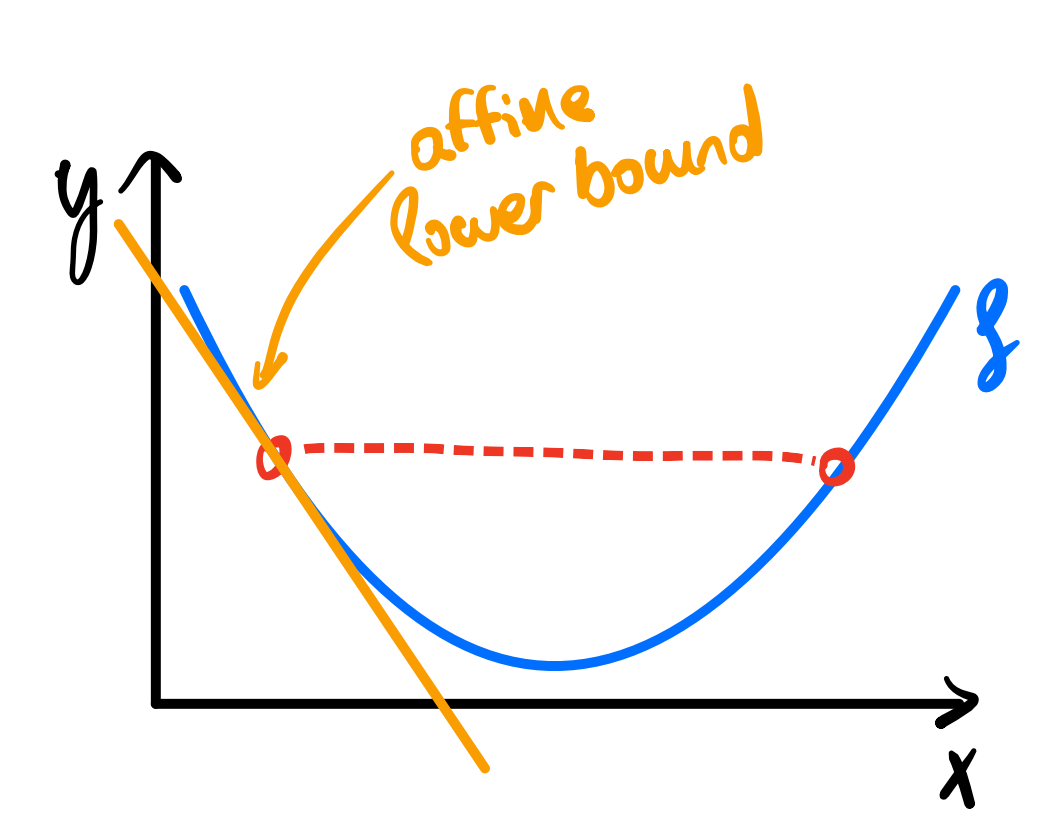
\includegraphics[width=3cm]{notes/figures/1st_order_characterization.png}
\caption{The first-order characterization characterizes convexity in terms of affine lower bounds.}
\end{marginfigure}
\begin{thm}[First-order characterization of convexity] Consider a differentiable function $f: \sS \to \R$. Then, $f$ is convex iff \begin{align}
    f(\vy) \geq f(\vx) + \trans{\grad f(\vx)}(\vy - \vx)
\end{align} for all $\vx, \vy \in \sS$. Moreover, $f$ is strictly convex iff \begin{align}
    f(\vy) > f(\vx) + \trans{\grad f(\vx)}(\vy - \vx)
\end{align}
\end{thm}
\begin{proof} We first prove the statement about convexity. \begin{itemize}
    \item ``$\Rightarrow$'': Fix any $\vx, \vy \in \sS$. As $f$ is convex, \begin{align*}
        f((1-\theta)\vx + \theta\vy) \leq (1-\theta)f(\vx) + \theta f(\vy),
    \end{align*} for all $\theta \in [0,1]$. We can rearrange to, \begin{align*}
        f(\underbrace{(1-\theta)\vx + \theta\vy}_{\vx + \theta(\vy - \vx)}) - f(\vy) \leq \theta(f(\vx) - f(\vy)).
    \end{align*} Dividing by $\theta$ yields, \begin{align*}
        \frac{f(\vx + \theta(\vy - \vx)) - f(\vx)}{\theta} \leq f(\vy) - f(\vx).
    \end{align*} Taking the limit $\theta \to 0$ on both sides gives the directional derivative at $\vx$ in direction $\vy - \vx$, \begin{align*}
        \trans{\grad f(\vx)}(\vy - \vx) = D f(\vx)[\vy - \vx] \leq f(\vy) - f(\vx).
    \end{align*}
    
    \item ``$\Leftarrow$'': Fix any $\vx, \vy \in \sS$ and let $\vz \defeq \theta\vy + (1-\theta)\vx$. We have, \begin{align*}
        f(\vy) &\geq f(\vz) + \trans{\grad f(\vz)}(\vy - \vz), \quad\text{and} \\
        f(\vx) &\geq f(\vz) + \trans{\grad f(\vz)}(\vx - \vz).
    \end{align*} We also have $(1-\theta)(\vy-\vx) = \vy - \vz$ and $\theta(\vy - \vx) = \vx - \vz$. Hence, \begin{align*}
        \theta f(\vy) + (1-\theta) f(\vx) &\geq f(\vz) + \trans{\grad f(\vz)}(\underbrace{\theta(\vy - \vz) + (1-\theta)(\vx - \vz)}_{0}) \\
        &= f(\theta\vy + (1-\theta)\vx).
    \end{align*}
\end{itemize}

Finally, observe that the statement about strict convexity can be proven analogously by making the inequalities strict.
\end{proof}

\begin{thm} Let $f: \sS \to \R$ be a convex and differentiable function. Then, if $\vx \in \sS$ is a stationary point of $f$, then $\vx$ is a global minimum of $f$.
\end{thm}
\begin{proof} By the first-order characterization of convexity, we have for any $\vy \in \sS$, \begin{align*}
    f(\vy) \geq f(\vx) + \underbrace{\trans{\grad f(\vx)}}_{0}(\vy - \vx) = f(\vx). &\qedhere
\end{align*}
\end{proof}

\section{Second-order Characterization of Convexity}

\begin{thm}[Second-order characterization of convexity] Consider a twice continuously differentiable function $f: \sS \to \R$.\footnote{Here we need our assumption that $\sS$ is open.} \begin{enumerate}
    \item $f$ is convex iff $\mH_f(\vx)$ is positive semi-definite for all $\vx \in \sS$.
    \item $f$ is strictly convex iff $\mH_f(\vx)$ is positive definite for all $\vx \in \sS$.
\end{enumerate}
\end{thm}
\begin{proof} We first prove the statement about convexity. \begin{itemize}
    \item ``$\Leftarrow$'': Fix any $\vx, \vy \in \sS$. By the second-order form of Taylor's theorem, \begin{align*}
        f(\vy) &= f(\vx) + \trans{\grad f(\vx)}(\vy - \vx) + \frac{1}{2}\underbrace{\trans{(\vy - \vx)}\mH_f(\vz)(\vy - \vx)}_{\geq 0} \\
        &\geq f(\vx) + \trans{\grad f(\vx)}(\vy - \vx),
    \end{align*} for some $\vz \in [\vx,\vy]$. This coincides with the first-order characterization of convexity.
    
    \item ``$\Rightarrow$'': Fix any $\vx \in \sS$ and $\vd \in \R^n$. Note that, as $\sS$ is open, for small enough $\lambda \in [-\epsilon,\epsilon] \setminus \{0\}$, $\vx + \lambda\vd \in \sS$. We have, \begin{align*}
        0 &\leq f(\vx + \lambda\vd) - [f(\vx) + \lambda \trans{\grad f(\vx)}\vd] \margintag{using the first-order characterization of convexity} \\
        &= \frac{1}{2}\lambda^2\trans{\vd}\mH_f(\vx)\vd + o(\lambda^2 \norm{\vd}_2^2). \margintag{using a second-order expansion}
    \end{align*} Multiplying both sides by $\nicefrac{2}{\lambda^2}$ and taking the limit $\lambda \to 0$, we obtain, \begin{align*}
        0 \leq \trans{\vd}\mH_f(\vx)\vd + \lim_{\lambda \to 0}\frac{o(\lambda^2 \norm{\vd}_2^2)}{\lambda^2} = \trans{\vd}\mH_f(\vx)\vd.
    \end{align*}
\end{itemize}

The statement about strict convexity follows by using the first-order characterization of strict convexity instead and replacing inequalities with strict inequalities.
\end{proof}
    % !TeX root = ../main.tex
% Add the above to each chapter to make compiling the PDF easier in some editors.

\chapter{Gradient Descent}

Gradient descent\index{gradient descent} is a method for solving minimization problems such as \cref{eq:optimization_problem}.

\begin{defn}[Approximate solution]
We say that a solution $\vx_k$ to the optimization problem $\min_{\vx \in \sS} f(\vx)$ is \emph{$\epsilon$-approximate}\index{approximate solution} iff \begin{align}
    f(\vx_k) - f(\s{\vx}) \leq \epsilon
\end{align} for some $\epsilon > 0$, where $\s{\vx} \in \argmin_{\vx \in \sS} f(\vx)$.
\end{defn}

For this chapter, we assume that the optimization problem is unconstrained, i.e., $\sS = \R^n$. In \cref{cha:lagrange_multipliers_duality}, we explore how we can solve constrained optimization problems using Lagrange multipliers.

The idea of gradient descent is to iteratively take a step in the opposite direction of the gradient starting from some initial point $\vx_0 \in \R^n$, \begin{align}
    \vx_{i+1} \gets \vx_i - \alpha \grad f(\vx_i),
\end{align} where $\alpha > 0$ is some learning rate.
\begin{marginfigure}
TBD
% \centering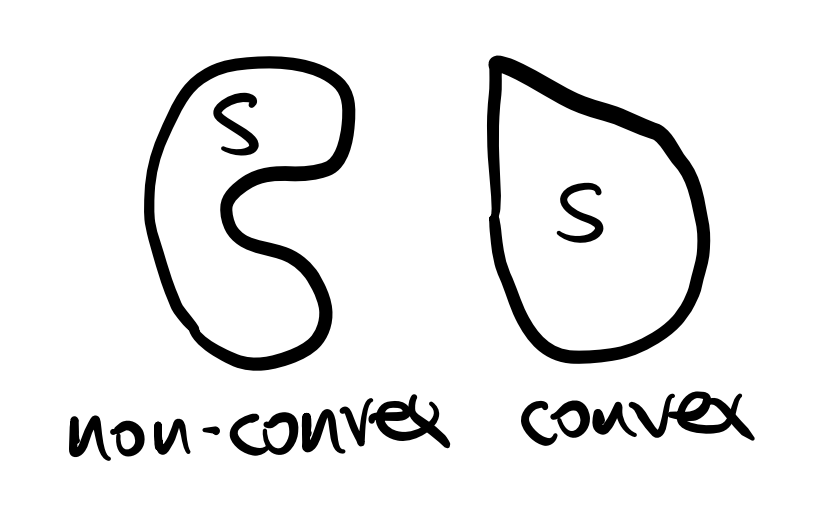
\includegraphics[width=4cm]{notes/figures/convex_set.png}
\caption{Non-convex function.}
\end{marginfigure}

When does gradient descent work? Clearly, we need that $f$ is convex, otherwise gradient descent might not converge to the global minimum at all. But this is not enough! We also need to ensure that the gradient of $f$ does not change arbitrarily when making very small steps, else the gradient direction would not be useful for us. This property is often called \emph{smoothness}.

\begin{marginfigure}
TBD
% \centering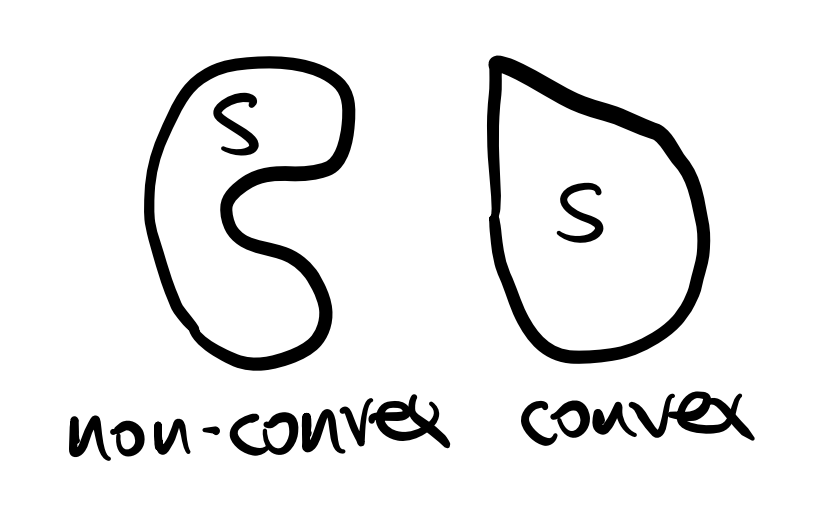
\includegraphics[width=4cm]{notes/figures/convex_set.png}
\caption{Function whose gradient is close to zero at a non-optimal point.}
\end{marginfigure}
Finally, it is intuitively clear that we can do much better when we can ensure that the gradient of $f$ is only close to zero around its minimum. If not, that is, we (almost) have ``saddle points'', the step size of gradient descent will slow down and depending on the stopping criterion we might even return a point that is not the minimizer. To exclude such functions from our analysis, we often assume that $f$ satisfies the \emph{PL condition}, or else is \emph{strongly convex}.

You can think of smoothness as providing a quadratic upper bound to our function, whereas strong convexity provides a quadratic lower bound.

\section{Smoothness}

\begin{defn}[Smoothness] Let $f: \sS \to \R$ be continuously differentiable. We say, $f$ is \emph{$\beta$-smooth}\index{smoothness} for some $\beta > 0$ iff for any $\vx, \vy \in \sS$ \begin{align}
    \norm{\grad f(\vx) - \grad f(\vy)}_2 \leq \beta \norm{\vx - \vy}_2.
\end{align} In other words, the gradient of $f$ is $\beta$-Lipschitz.
\end{defn}
\begin{lem}
A twice continuously differentiable function $f: \sS \to \R$ is $\beta$-smooth iff for any $\vx \in \sS$, $\lambda_{\max}(\mH_f(\vx)) \leq \beta$.
\end{lem}
\begin{proof}
TBD
\end{proof}
\begin{lem}
A continuously differentiable function $f: \sS \to \R$ is $\beta$-smooth iff for any $\vx, \vy \in \sS$, \begin{align}
    f(\vy) \leq f(\vx) + \trans{\grad f(\vx)}(\vy - \vx) + \frac{\beta}{2}\norm{\vy - \vx}_2^2.
\end{align}
\end{lem} In words, $f(\vy)$ is upper bounded by a quadratic approximation based at $f(\vx)$.
\begin{proof}
TBD
\end{proof}

\subsection{Analysis of Gradient Descent}

A natural approach is to choose the gradient step of each iteration such that we minimize the upper bound (due to smoothness) based at the current solution, \begin{align}
    \grad_\vdelta \parentheses*{f(\vx_i) + \trans{\grad f(\vx_i)}\vdelta + \frac{\beta}{2}\norm{\vdelta}_2^2} = \grad f(\vx_i) + \beta\vdelta \overset{!}{=} 0,
\end{align} which is achieved for $\vdelta = -\frac{1}{\beta}\grad f(\vx_i)$. Thus, \begin{align}
    f(\vx_{i+1}) - f(\vx_i) &\leq \underbrace{\trans{\grad f(\vx_i)}\vdelta}_{-\frac{1}{\beta}\norm{\grad f(\vx_i)}_2^2} + \underbrace{\frac{\beta}{2}\norm{\vdelta}_2^2}_{\frac{1}{2\beta}\norm{\grad f(\vx_i)}_2^2} = -\frac{1}{2\beta}\norm{\grad f(\vx_i)}_2^2.
\end{align} Moreover, due to the first-order characterization of convexity, \begin{align}
    f(\vx_i) - f(\s{\vx}) \leq \trans{\grad f(\vx_i)}(\vx_i - \s{\vx}) \leq \norm{\grad f(\vx_i)}_2 \norm{\vx_i - \s{\vx}}_2,
\end{align} where the second inequality follows from Cauchy-Schwarz. Combining the previous two inequalities, \begin{align}
    f(\vx_{i+1}) - f(\vx_i) \leq -\frac{1}{2\beta}\parentheses*{\frac{f(\vx_i) - f(\s{\vx})}{\norm{\vx_i - \s{\vx}}_2}}^2 \leq -\frac{1}{2\beta}\parentheses*{\frac{f(\vx_i) - f(\s{\vx})}{\norm{\vx_0 - \s{\vx}}_2}}^2. \margintag{using that $\norm{\vx_i - \s{\vx}}_2 \leq \norm{\vx_0 - \s{\vx}}_2$, which follows from $f$ decreasing in every iteration and convexity} \label{eq:gd_gap}
\end{align}

\begin{thm}[Convergence of gradient descent] Suppose $f: \R^n \to \R$ is convex and $\beta$-smooth. The gradient descent scheme, \begin{align}
    \vx_{i+1} \defeq \vx_i - \frac{1}{\beta}\grad f(\vx_i),
\end{align} yields an $\epsilon$-approximate solution $\vx_k$ for some \begin{align*}
    k \geq \frac{2\beta\norm{\vx_0 - \s{\vx}}_2^2}{\epsilon}.
\end{align*}
\end{thm}

\begin{proof} We prove $f(\vx_k) - f(\s{\vx}) \leq \frac{2\beta\norm{\vx_0 - \s{\vx}}_2^2}{k+1}$ by induction on the length of the computation $k$. Suppose $k = 0$, then by the smoothness of $f$, \begin{align*}
    f(\vx_0) \leq f(\s{\vx}) - \underbrace{\trans{\grad f(\s{\vx})}}_{\vZero}(\vx_0 - \s{\vx}) + \frac{\beta}{2}\norm{\vx_0 - \s{\vx}}_2^2.
\end{align*} For the induction step, suppose that the statement holds for the $k$-th iterate. We write $\dgap_i \defeq f(\vx_i) - f(\s{\vx})$. Using \cref{eq:gd_gap}, \begin{align*}
    \dgap_{k+1} - \dgap_k \leq -\frac{\dgap_k^2}{2\beta\norm{\vx_0 - \s{\vx}}_2^2}.
\end{align*} Dividing by $\dgap_k \cdot \dgap_{k+1}$ and using that $\dgap_{k+1} > 0$ and $\dgap_k \geq \dgap_{k+1}$, we have, \begin{align*}
    \frac{1}{\dgap_k} - \frac{1}{\dgap_{k+1}} \leq -\frac{\dgap_k^2}{2\beta\norm{\vx_0 - \s{\vx}}_2^2 \dgap_k \dgap_{k+1}} \leq -\frac{1}{2\beta\norm{\vx_0 - \s{\vx}}_2^2}.
\end{align*} Thus, \begin{align*}
    \frac{1}{\dgap_{k+1}} \geq \frac{1}{2\beta\norm{\vx_0 - \s{\vx}}_2^2} + \frac{1}{\dgap_k} \geq \frac{(k+1) + 1}{2\beta\norm{\vx_0 - \s{\vx}}_2^2} \margintag{using the induction hypothesis} &\qedhere
\end{align*}
\end{proof}

\section{Strong Convexity}

We can improve our analysis, when we assume that $f$ is strongly convex, that is lower bounded by a quadratic. Intuitively, this ensures that our steps are large when we are far away from the optimum.

\begin{defn}[Strong convexity] Let $f: \sS \to \R$ be continuously differentiable. We say, $f$ is \emph{$\mu$-strongly convex}\index{strong convexity} for some $\mu > 0$ iff for any $\vx,\vy \in \sS$, \begin{align}
    f(\vy) \geq f(\vx) + \trans{\grad f(\vx)}(\vy - \vx) + \frac{\mu}{2}\norm{\vy - \vx}_2^2.
\end{align}
\end{defn}
\begin{lem}
A twice continuously differentiable function $f: \sS \to \R$ is $\mu$-strongly convex iff for any $\vx \in \sS$, $\lambda_{\min}(\mH_f(\vx)) \geq \mu$.
\end{lem}
\begin{proof}
TBD
\end{proof}
\begin{cor}
If $f$ is $\beta$-smooth and $\mu$-strongly convex, then $\mu \leq \beta$.
\end{cor}

\begin{defn}[Condition number] We call $\kappa \defeq \frac{\beta}{\mu}$ the \emph{condition number}\index{condition number} of a function $f$ that is $\beta$-smooth and $\mu$-strongly convex.
\end{defn}

Often, a weaker condition known as \emph{PL condition} is sufficient to design fast algorithms.

\begin{defn}[Polyak-Łojasiewicz inequality]\index{Polyak-Łojasiewicz inequality} A continuously differentiable function $f: \sS \to \R$ satisfies the PL inequality with parameter $\mu > 0$ iff \begin{align}
    \frac{1}{2}\norm{\grad f(\vx)}_2^2 \geq \mu (f(\vx) - f(\s{\vx})),
\end{align} where $\s{\vx} \in \argmin_{\vx \in \sS} f(\vx)$.
\end{defn}\noindent Intuitively, the norm of the gradient is tied to the suboptimality of the current solution.

\begin{lem}
Let $f: \sS \to \R$ be continuously differentiable and $\mu$-strongly convex. Then, $f$ satisfies the PL condition.
\end{lem}
\begin{proof}
As $f$ is $\mu$-strongly convex, \begin{align*}
    f(\vy) \geq f(\vx) + \trans{\grad f(\vx)}(\vy - \vx) + \frac{\mu}{2}\norm{\vy - \vx}_2^2,
\end{align*} for any $\vx, \vy \in \sS$. Taking the minimum with respect to $\vy$ on both sides yields, \begin{align*}
    f(\s{\vx}) \geq f(\vx) - \frac{1}{2\mu}\norm{\grad f(\vx)}_2^2,
\end{align*} as the right-hand side is minimized for $\vy = \vx - \frac{1}{\mu}\grad f(\vx)$. The PL inequality follows from rearranging the terms.
\end{proof}

\subsection{Analysis of Gradient Descent}

\begin{thm}[Convergence of gradient descent with a strongly convex objective] Suppose $f: \R^n \to \R$ is $\mu$-strongly convex and $\beta$-smooth. The gradient descent scheme, \begin{align}
    \vx_{i+1} \defeq \vx_i - \frac{1}{\beta}\grad f(\vx_i),
\end{align} yields an $\epsilon$-approximate solution $\vx_k$ for some \begin{align*}
    k \geq \kappa\log\parentheses*{\frac{\beta\norm{\vx_0 - \s{\vx}}_2^2}{2\epsilon}}.
\end{align*}
\end{thm}
\begin{proof}
See the first graded homework.
\end{proof}

\begin{rmk}
It turns out that the PL condition is sufficient to establish this convergence rate.
\end{rmk}

\section{Acceleration}

We can get an algorithm that converges substantially faster than vanilla gradient descent, using a method known as \emph{accelerated gradient descent}\index{accelerated gradient descent}. The key idea is to --- instead of only tracking the upper bound that is due to smoothness --- also use track lower bounds. In one iteration we might not make much progress in terms of reducing the upper bound (that is, improving our current solution), but instead increase the upper bound, which still reduces the error.

\begin{thm}[Convergence of accelerated gradient descent] Suppose $f: \R^n \to \R$ is convex and $\beta$-smooth. The accelerated gradient descent scheme, \begin{align}\begin{split}
    a_i &\defeq \frac{i+1}{2}, \quad A_i \defeq \frac{(i+1)(i+2)}{4} \\
    \vv_0 &\defeq \vx_0 - \frac{1}{2\beta} \grad f(\vx_0) \\
    \vy_i &\defeq \vx_i - \frac{1}{\beta} \grad f(\vx_i) \\
    \vx_{i+1} &\defeq \frac{A_i\vy_i + a_{i+1}\vv_i}{A_{i+1}} \\
    \vv_{i+1} &\defeq \vv_i - \frac{a_{i+1}}{\beta} \grad f(\vx_{i+1}),
\end{split}\end{align} yields an $\epsilon$-approximate solution $\vx_k$ for some \begin{align*}
    k \geq \sqrt{\frac{2\beta\norm{\vx_0 - \s{\vx}}_2^2}{\epsilon}}.
\end{align*}
\end{thm} Here, $\vy_i$ is the current solution (i.e., an upper bound), $\vv_i$ is a lower bound, and $\vx_i$ a point that trades improving the lower/upper bounds.

\begin{proof}
TBD
\end{proof}

\subsection{Acceleration with Strongly Convex Objectives}

\begin{thm}[Convergence of accelerated gradient descent with a strongly convex objective] Suppose $f: \R^n \to \R$ is $\mu$-strongly convex and $\beta$-smooth. The accelerated gradient descent scheme, \begin{align}\begin{split}
    \vy_0 &\defeq \vx_0 \\
    \vy_{i+1} &\defeq \vx_i - \frac{1}{\beta} \grad f(\vx_i) \\
    \vx_{i+1} &\defeq (1+\theta)\vy_{i+1} + \theta\vy_i
\end{split}\end{align} for $\theta \defeq \frac{\sqrt{\kappa} - 1}{\sqrt{\kappa} + 1}$ yields an $\epsilon$-approximate solution $\vx_k$ for some \begin{align*}
    k \geq \sqrt{\kappa}\log\parentheses*{\frac{\beta\norm{\vx_0 - \s{\vx}}_2^2}{\epsilon}}.
\end{align*}
\end{thm}
\begin{proof}
See the first graded homework.
\end{proof}

    % !TeX root = ../main.tex
% Add the above to each chapter to make compiling the PDF easier in some editors.

\chapter{Non-Euclidean Geometries}

\section{Mirror Descent}
    % !TeX root = ../main.tex
% Add the above to each chapter to make compiling the PDF easier in some editors.

\chapter{Lagrange Multipliers and Duality}\label{cha:lagrange_multipliers_duality}

\section{Separating Hyperplanes}

\begin{defn}[Hyperplane] A \emph{hyperplane}\index{hyperplane} of dimension $n$ is the subset, \begin{align}
    \sH(\vn,\mu) \defeq \{\vx \in \R^n \mid \trans{\vn}\vx = \mu\},
\end{align} for some \emph{normal}\index{normal vector} $\vn \in \R^n \setminus \{\vZero\}$ and \emph{threshold} $\mu \in \R$.
\end{defn}

Every hyperplane divides $\R^n$ into two half-spaces $\{\vx \mid \trans{\vn}\vx \leq \mu\}$ and $\{\vx \mid \trans{\vn}\vx \geq \mu\}$. It separates two sets, if they lie in different half-spaces.

\begin{defn}[Separating hyperplane] We say a hyperplane $\sH$ \emph{separates}\index{separating hyperplane} two sets $\sA, \sB$ iff \begin{align}\begin{split}
    \forall a \in \sA: \trans{\vn}\va &\leq \mu \quad\text{and} \\
    \forall b \in \sB: \trans{\vn}\vb &\geq \mu.
\end{split}\end{align} If the inequalities are strict, we say that $\sH$ \emph{strictly} separates $\sA$ and $\sB$.
\end{defn}

If $\sA, \sB$ are non-convex, we are not guaranteed that a separating hyperplane exists (e.g., a point cannot be separated from a ring around it). However, if we assume that $\mA$ and $\mB$ are convex, a separating hyperplane always exists.

\begin{fct}[Separating hyperplane theorem]\index{Separating hyperplane theoerm} Given two disjoint and non-empty convex subsets $\sA, \sB \subseteq \R^n$, there exists a separating hyperplane.
\end{fct}

However, it is not true that there always exists a strictly separating hyperplane. Consider $\sA \defeq \{(x,y) \mid x \leq 0\}$ and $\sB \defeq \{(x,y) \mid x > 0 \text{ and } y \geq \frac{1}{x}\}$. Clearly they are disjoint and convex; however, the only separating hyperplane is $\sH = \{(x,y) \mid x = 0\}$, which intersects $\sA$.
\begin{marginfigure}
TBD
% \centering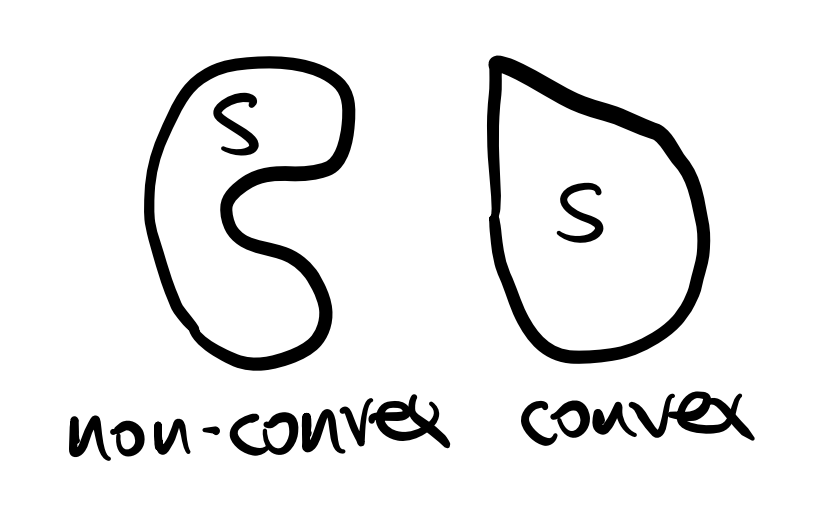
\includegraphics[width=4cm]{notes/figures/convex_set.png}
\caption{Example where no strictly separating hyperplane exists.}
\end{marginfigure}

When we also assume that $\sA$ and $\sB$ are closed and bounded, a strictly separating hyperplane always exists.

\begin{thm}[Separating hyperplane theorem; closed, bounded sets] Given two disjoint, closed, bounded, and non-empty convex subsets $\sA, \sB \subseteq \R^n$, there exists a strictly separating hyperplane.

If $\vc \in \sA, \vd \in \sB$ are minimizers of $\min_{\va \in \sA,\ \vb \in \sB} \norm{\va - \vb}_2$, then one such hyperplane is given by, \begin{align}
    \vn \defeq \vd - \vc \quad\text{and}\quad \mu \defeq \frac{1}{2}\parentheses*{\norm{\vd}_2^2 - \norm{\vc}_2^2}.
\end{align}
\begin{marginfigure}
TBD
% \centering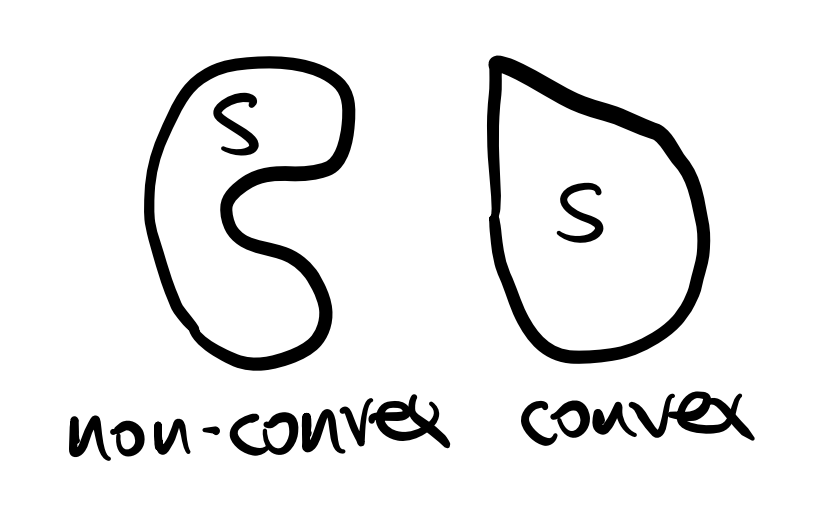
\includegraphics[width=4cm]{notes/figures/convex_set.png}
\caption{Illustration of strictly separating hyperplane.}
\end{marginfigure}
\end{thm}
\begin{proof}
We want to show that $\trans{\vn}\vb > \mu$ for all $\vb \in \sB$. Then, $\trans{\vn}\va < \mu$ for all $\va \in \sA$ follows by symmetry. We have, \begin{align*}
    \trans{\vn}\vd - \mu &= \trans{(\vd - \vc)}\vd - \frac{1}{2}\parentheses*{\norm{\vd}_2^2 - \norm{\vc}_2^2} \\
    &= \norm{\vd}_2^2 - \trans{\vd}\vc - \frac{1}{2}\norm{\vd}_2^2 + \frac{1}{2}\norm{\vc}_2^2 \\
    &= \frac{1}{2}\norm{\vd - \vc}_2^2 > 0. \margintag{using the asusmption that $\sA,\sB$ are disjoint, close, and bounded, their distance is positive}
\end{align*} Suppose for a contradiction that there exists a $\vu \in \sB$ such that $\trans{\vn}\vu - \mu \leq 0$.

Consider the line defined by the distance minimizer $\vd$ and the point on the ``wrong side'' $\vu$, $\vb(\lambda) \defeq \vd + \lambda(\vu - \vd)$. Taking the derivative of the distance between $\vb(\lambda)$ and $\vc$ and evaluating it at $\lambda = 0$ (which is when $\vb(\lambda) = \vd$), we obtain, \begin{align*}
    \left.\odv{}{\lambda}\norm{\vb(\lambda)-\vc}_2^2\right\vert_{\lambda=0} &= \left.2 \trans{(\vd - \lambda\vd + \lambda\vu - \vc)}(\vu-\vd)\right\vert_{\lambda=0} \\
    &= 2 \trans{(\vd - \vc)}(\vu - \vd).
\end{align*} However, \begin{align*}
    \trans{\vn}\vu - \mu = \trans{(\vd - \vc)}(\vu - \vd) + \underbrace{\trans{\vn}\vd - \mu}_{>0} \leq 0,
\end{align*} implies that $\trans{(\vd - \vc)}(\vu - \vd)$, and hence, the gradient are negative, which contradicts the minimality of $\vd$.
\end{proof}

\section{Lagrange Multipliers and KKT Conditions}

We will now discuss how we can treat constraints in a convex optimization problem, \begin{align}
    \s{\alpha} \defeq \min_{\substack{\vy \in \R^n \\ \mA\vy = \vb \\ \vg(\vy) \leq \vZero}} f(\vy),
\end{align} where $f : \R^n \to \R$ is convex, $\mA \in \R^{m \times n}$, $\vb \in \R^m$, and we have $k$ convex constraints $g_i : \R^n \to \R$.

\begin{rmk}
The linear constraints $\mA\vy = \vb$ are not necessary, as they can also be modeled using the (convex) constraints $\mA\vy - \vb \leq \vZero$ and $\vb - \mA\vy \leq 0$. We include them here to see later that programs with only linear constraints can be handled in a slightly different way.
\end{rmk}

We call this optimization problem the \emph{primal problem}\index{primal problem} and we will later see that it has an associated dual problem. We say that $\vy \in \R^n$ is \emph{primal feasible}\index{primal feasible} iff $\mA\vy = \vb$ and $\vg(\vy) \leq \vZero$.

\begin{marginfigure}
TBD
% \centering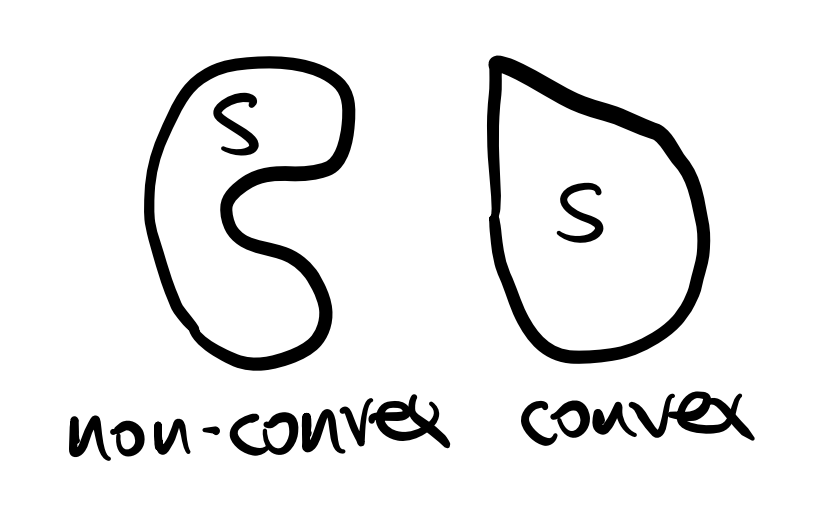
\includegraphics[width=4cm]{notes/figures/convex_set.png}
\caption{Illustration of simple constrained optimization.}
\end{marginfigure}
In the following, we want to answer the question: ``When is a feasible point optimal?'' To simplify things a bit, let us consider the optimization problem of minimizing $f$ under the single constraint $g$. Suppose we know the feasible optimum $\s{\vy}$. Then for infinitesimal $\vdelta$, if $\vdelta \perp \grad g(\s{\vy})$, then $\s{\vy} + \vdelta$ and $\s{\vy} - \vdelta$ are feasible. But then we must have that $\vdelta \perp \grad f(\s{\vy})$, or else one direction would improve the objective. This tells us that, \begin{align*}
    \trans{\vdelta}\grad f(\s{\vy}) = 0 = \trans{\vdelta}\grad g(\s{\vy}),
\end{align*} and hence, there exists some $\lambda \in \R$ such that $\grad f(\s{\vy}) = \lambda \grad g(\s{\vy})$. This is the fundamental intuition behind a \emph{Lagrange multiplier}: the gradient of the objective at an optimal point is a linear combination of the gradients of the (tight) constraints.

We say that the constraint $g_i$ is \emph{tight}\index{tight constraint} at $\vy$ iff $g_i(\vy) = 0$.

% \section{Fenchel Conjugates}
    % !TeX root = ../main.tex
% Add the above to each chapter to make compiling the PDF easier in some editors.

\chapter{Newton's Method}

    \part{Spectral Graph Theory}\label{part3}
    % !TeX root = ../main.tex
% Add the above to each chapter to make compiling the PDF easier in some editors.

\chapter{Introduction to Spectral Graph Theory}

Spectral graph theory studies graphs through linear algebra. The fundamental object that we will work with is the Laplacian matrix that we introduced in \cref{defn:laplacian_matrix}.

\section{Eigenvalues of the Laplacian Matrix}

\begin{lem}
Denote by $\sX_1 \cup \dots \cup \sX_k = V$ the connected components of a graph $G$. Then we have for the Laplacian matrix $\mL$ of $G$, \begin{align}
    \ker{\mL} = \vspan\{\vOne_{\sX_1}, \dots, \vOne_{\sX_k}\},
\end{align} where $\vOne_{\sX}(v) = \Ind{v \in \sX}$. In particular, $\ker{\mL} = \vspan\{\vOne\}$ if $G$ is connected.
\end{lem}
\begin{proof}
TBD
\end{proof}
\begin{cor}
When $G$ has $k$ connected components, then $\lambda_i(\mL) = 0$ for all $i \in [k]$.
\end{cor}

In the following, we will study connected graphs. If a graph consists of multiple connected components, we may study each individually.

\begin{lem}
$\mL \preceq 2\mD$.
\end{lem}
\begin{proof} It can be shown that $\mD + \mA \succeq \mZero$,\footnote{The proof is similar to the proof that $\mL = \mD - \mA \succeq \mZero$. $\mD + \mA$ is also called the \emph{signless Laplacian matrix}\index{signless Laplacian matrix} and is an interesting object in its own right: its eigenvalues can be used to count edges and identify bipartite components.} so, $\mD \succeq -\mA$, and hence, $\mL \preceq 2\mD$.
\end{proof}

\subsection{Electrical Energy}

\begin{lem}
For any voltages $\vx \in \R^{|\sV|}$, \begin{align}
    \lambda_2(\mL) \norm{\vx}_2^2 \leq \spa{E}(\vx) \leq \lambda_n(\mL) \norm{\vx}_2^2.
\end{align}
\end{lem}
\begin{proof}
TBD
\end{proof}

\begin{lem}
Voltages $\vx \in \R^{|\sV|}$ routing demands $\vd \perp \vOne$ satisfy, \begin{align}
    \frac{\norm{\vd}_2^2}{\lambda_n(\mL)} \leq \spa{E}(\vx) \leq \frac{\norm{\vd}_2^2}{\lambda_2(\mL)}.
\end{align}
\end{lem}
\begin{proof}
TBD
\end{proof}

\subsection{Useful Inequalities}

\begin{lem}[Path inequality]\index{path inequality} We have that \begin{align}
    (n-1) P_n \succeq G_{1,n},
\end{align} where $P_n$ is the unit weight path graph on $n$ vertices and $G_{i,j}$ is the unit weight graph on $n$ vertices with the single edge $\{i,j\}$.
\end{lem}
\begin{proof}
Fix any $\vx \in \R^n$ and let $\vDelta(i) \defeq \vx(i+1) - \vx(i)$. We have, \begin{align*}
    \trans{\vx}G_{1,n}\vx &= (\vx(n) - \vx(1))^2 \\
    &= \parentheses*{\sum_{i=1}^{n-1} \vDelta(i)}^2 \\
    &= (\trans{\vOne_{n-1}}\vDelta)^2 \\
    &\leq \norm{\vOne_{n-1}}_2^2 \norm{\vDelta}_2^2 \margintag{using Cauchy-Schwarz} \\
    &= (n-1) \sum_{i=1}^{n-1} \vDelta(i)^2 \\
    &= (n-1) \sum_{i=1}^{n-1} (\vx(i+1) - \vx(i))^2 \\
    &= (n-1)\trans{\vx}P_n\vx. \qedhere
\end{align*}
\end{proof}

\begin{lem}
For any unit weight graph $G$ on $n$ vertices with diameter\footnote{The \emph{diameter}\index{diameter} of a graph is the length of its longest path.} $D$, \begin{align}
    \lambda_2(G) \geq \frac{1}{nD}.
\end{align}
\end{lem}
\begin{proof} We denote by $G^{i,j}$ the subgraph of $G$ consisting of the shortest $i-j$ path. We have, \begin{align*}
    K_n = \sum_{i < j} G_{i,j} &\preceq \sum_{i<j} \underbrace{(j-i)}_{\leq D} \underbrace{G^{i,j}}_{\subseteq G} \margintag{analogously to the path inequality} \\
    &\preceq n^2 D G.
\end{align*} Thus, $n^2 D \lambda_2(G) \geq \lambda_2(K_n) = n$, and hence, $\lambda_2(G) \geq \frac{1}{nD}$.
\end{proof}

\section{Examples}

\begin{lem}[Spectrum of the complete graph] \begin{align}
    \lambda_2(K_n) = \dots = \lambda_n(K_n) = n.
\end{align}
\end{lem}
\begin{proof} We have, $\mA = \vOne\trans{\vOne} - \mI$ and $\mD = (n-1)\mI$, so $\mL = n\mI - \vOne\trans{\vOne}$. For any $\vx \perp \vOne$, $\mL\vx = n\vx$.
\end{proof}

We now want to better understand $\lambda_2$ and $\lambda_n$ for some common graphs. The tools we will use are the following: \begin{itemize}
    \item \underline{to lower bound $\lambda_2(G)$:} Relate the eigenvalues of $K_n$ and $G$, yielding $K_n \preceq f(n) G$. Knowing that $\lambda_2(K_n) = n$, we have, $f(n) \lambda_2(G) \geq n$, and hence, $\lambda_2(G) \geq \frac{n}{f(n)}$.
    \item \underline{to upper bound $\lambda_2(G)$:} Due to Courant-Fischer, \begin{align*}
        \lambda_2(G) = \min_{\substack{\vx \perp \vOne \\ \vx \neq \vZero}} \frac{\trans{\vx}\mL\vx}{\trans{\vx}\vx} \leq \frac{\trans{\vy}\mL\vy}{\trans{\vy}\vy},
    \end{align*} for any $\vy \perp \vOne, \vy \neq \vZero$. We can therefore find a so-called \emph{test vector}\index{test vector} $\vy$ with these properties.
    \item \underline{to lower bound $\lambda_n(G)$:} Similarly, due to Courant-Fischer, \begin{align*}
        \lambda_n(G) = \max_{\vx \neq \vZero} \frac{\trans{\vx}\mL\vx}{\trans{\vx}\vx} \geq \frac{\trans{\vy}\mL\vy}{\trans{\vy}\vy},
    \end{align*} for any $\vy \neq \vZero$.
    \item \underline{to upper bound $\lambda_n(G)$:} Using that $\mL \preceq 2 \mD$, we have, $\lambda_n(G) \leq 2 \max_{v \in \sV} \vd(v)$, where $\vd(v)$ is the weighted degree of $v$.
\end{itemize}

\subsection{Path Graph}

\begin{lem} $\lambda_2(P_n) = \Theta\parentheses*{\frac{1}{n^2}}$.
\end{lem}
\begin{proof}
TBD
\end{proof}

\begin{lem} $\lambda_n(P_n) \in [1,4]$.
\end{lem}
\begin{proof}
TBD
\end{proof}

\subsection{Complete Binary Tree}

\begin{lem} $\lambda_2(T_d) = \Theta\parentheses*{\frac{1}{n}}$.
\end{lem}
\begin{proof}
TBD
\end{proof}

\begin{lem} $\lambda_n(T_d) \in [1,6]$.
\end{lem}
\begin{proof}
TBD
\end{proof}
    % !TeX root = ../main.tex
% Add the above to each chapter to make compiling the PDF easier in some editors.

\chapter{Conductance and Expanders}

\section{Conductance}

\begin{defn}[Volume] The \emph{volume}\index{volume} of a set of vertices $\sS \subseteq \sV$ is the sum of weighted degrees, \begin{align}
    \vol(S) \defeq \sum_{v \in \sS} \vd(v) = \trans{\vOne_\sS}\vd = \trans{\vOne_\sS}\mD\vOne_\sS.
\end{align}
\end{defn}

A \emph{cut}\index{cut} $(\sS, \sV \setminus \sS)$ is a proper subset of vertices, $\emptyset \subset \sS \subset \sV$ partitioning vertices into two sets $\sS$ and $\sV \setminus \sS$.

\begin{defn}[Value of a cut] The \emph{value}\index{cut value} of a cut $(\sS, \sV \setminus \sS)$ is the sum of weights of crossing edges, \begin{align}\begin{split}
    c(\sS) &\defeq \sum_{\substack{\{a,b\} \in \sE \\ a \in \sS,\ b \in \sV \setminus \sS}} \vw(\{a,b\}) \\
    &= \sum_{\{a,b\}\in\sE} \vw(\{a,b\}) [\vOne_\sS(a) - \vOne_\sS(b)]^2 = \trans{\vOne_\sS}\mL\vOne_\sS.
\end{split}\end{align}
\end{defn}

\begin{defn}[Conductance of a cut] The \emph{conductance}\index{conductance} of a cut $(\sS, \sV \setminus \sS)$ is, \begin{align}
    \phi(\sS) \defeq \frac{c(\sS)}{\min\{\vol(\sS), \vol(\sV \setminus \sS)\}} = \phi(\sV \setminus \sS) \in [0,1],
\end{align} where, if the graph has unit weights, $c(\sS) = |\sE(\sS, \sV \setminus \sS)|$ counts the number of crossing edges.
\end{defn}

\begin{rmk}
If $\vol(\sS) \leq \vol(\sV \setminus \sS)$, then we can write \begin{align}
    \phi(\sS) = \frac{\trans{\vOne_\sS}\mL\vOne_\sS}{\trans{\vOne_\sS}\mD\vOne_\sS}.
\end{align}
\end{rmk}

\begin{defn}[Conductance of a graph]The \emph{conductance} of a graph $G$ is the smallest conductance of all cuts, \begin{align}
    \phi(G) \defeq \min_{\emptyset \subset \sS \subset \sV} \phi(S).
\end{align}
\end{defn} Thus, $\phi(G)$ is small if there is a ``good'' cut (with few crossing edges relative to the volume of the parts). In contrast, if $\phi(G)$ is large, then $G$ is well-connected, i.e., there is no ``good'' cut.

\begin{defn}[Expander and expander decomposition] For any $\phi \in (0,1]$, if $\phi(G) \geq \phi$, then $G$ is called a \emph{$\phi$-expander}\index{expander}.

A \emph{$\phi$-expander decomposition}\index{expander decomposition} of \emph{quality}\index{quality} $q$ is a partition of the vertex set $\sV = \sX_1 \cup \dots \cup \sX_k$ such that \begin{enumerate}
    \item $G[\sX_i]$ is a $\phi$-expander; and
    \item the number of edges not contained in any $G[\sX_i]$ is at most $q \phi m$, i.e. only ``few'' edges cross the parts.
\end{enumerate}
\end{defn}

In \cref{cha:expanders_using_max_flow}, we discuss how we can efficiently find an expander decomposition. Let us consider a few examples.

\begin{exc}\label{exc:expander_complete_graph}
$\phi(K_n) = \frac{n}{2(n-1)}$. So $K_n$ is a $\frac{1}{2}$-expander.
\end{exc}

\begin{exc}\label{exc:expander_path_graph}
$\phi(P_n) = \frac{1}{n-1}$. So $P_n$ is a $\frac{1}{n}$-expander.
\end{exc}

\begin{lem}
If $G$ is a connected $\phi$-expander with unit weights, then we have for the diameter $D$ of $G$, \begin{align}
    D = \LandauO{\frac{\log m}{\phi}}.
\end{align}
\end{lem}
\begin{proof}
Fix any pair of vertices $s,t \in \sV$. Let $B(s,d)$ be the closed ball around $s$ of radius $d$. Let $E(B(s,d))$ be the internal edge set of $B(s,d)$.

Observe that since $G$ is connected, we have $|E(B(s,0))| \geq 1$. Moreover, for each $d \geq 0$ where $|E(B(s,d))| \leq \frac{m}{2}$, we have by the definition of a $\phi$-expander that \begin{align*}
    |E(B(s,d), \sV \setminus B(s,d))| \geq \phi \cdot |E(B(s,d))|.
\end{align*} Thus, $|E(B(s,d+1))| \geq (1+\phi)|E(B(s,d))|$. Let $d_{\max}$ be the largest integer such that $|E(B(s,d_{\max}))| \leq \nicefrac{m}{2}$. We have $d_{\max} \leq \nicefrac{2\log m}{\phi}$ as otherwise, \begin{align*}
    |E(B(s,d_{\max}))| > (1+\phi)^{\nicefrac{2 \log m}{\phi}} \geq (1 + \nicefrac{\phi}{2} (\nicefrac{\phi}{2})^2)^{\nicefrac{2 \log m}{\phi}} \geq e^{\log m} = m, \margintag{using $e^x < 1 + x + x^2$ for $x < 1.79$}
\end{align*} which gives a contradiction to the fact that the number of edges in $G$ is $m$. Thus, for a radius of $\nicefrac{2 \log m}{\phi} + 1$, the ball centered at $s$ has more than $\nicefrac{m}{2}$ edges.

Finally, follow the same argument from $t$. As both balls contain more than $\nicefrac{m}{2}$ edges, they must intersect in at least one edge. But this implies that there is a $s$-$t$ path of length $\LandauO{\nicefrac{\log m}{\phi}}$.
\end{proof}

% \begin{thm}
% There is a procedure \textsc{CertifyOrCut($G, \phi$)} that either \begin{itemize}
%     \item certifies that $G$ is a $\phi$-expander; or
%     \item presents a cut $\sS$ such that $\phi(S) \leq \sqrt{2\phi}$.\footnote{Finding the best cut (i.e., a cut with conductance $\phi$) is NP-hard.}
% \end{itemize}
% \end{thm}
% \begin{proof}
% TBD
% \end{proof}

% \begin{thm}
% There is an algorithm that computes a $\phi$-expander decomposition of quality $q = \LandauO{\phi^{-\nicefrac{1}{2}} \log n}$ in time $\LandauO{m \log^c n}$ for some constant $c$.
% \end{thm}
% \begin{proof}
% TBD
% \end{proof}

\section{Cheeger's Inequality}

\begin{thm}[Cheeger's inequality]\index{Cheeger's inequality} We have for a graph $G$ and its normalized Laplacian matrix $\mN$, \begin{align}
    \frac{\lambda_2(\mN)}{2} \leq \phi(G) \leq \sqrt{2 \lambda_2(\mN)}.
\end{align}
\end{thm}\noindent In words, $\lambda_2(\mN)$ approximates the conductance $\phi(G)$ up to a square root. This is why we say that $\lambda_2(\mN)$ is a measure of connectivity of a graph.

\begin{proof}
TBD
\end{proof}

\section{Sparsity}

A concept related to conductance is the notion of \emph{sparsity}.

\begin{defn}[Sparsity] The \emph{sparsity}\index{sparsity} of a cut $(\sS, \sV \setminus \sS)$ is, \begin{align}
    \sigma(\sS) \defeq \frac{c(\sS)}{\min\{|\sS|, |\sV \setminus \sS|\}} = \sigma(\sV \setminus \sS) \in [0, \max_{v \in \sV} \vd(v)].
\end{align} The sparsity of a graph is again defined as the smallest sparsity of all cuts.
\end{defn}
\begin{rmk}
If $|\sS| \leq |\sV \setminus \sS|$, then we can write \begin{align}
    \sigma(\sS) = \frac{\trans{\vOne_\sS}\mL\vOne_\sS}{\trans{\vOne_\sS}\vOne_\sS}.
\end{align}
\end{rmk}

\begin{lem}
We have for any cut $(\sS, \sV \setminus \sS)$ in a connected unit weight graph that $\sigma(\sS) \geq \phi(\sS)$.
\end{lem}
\begin{proof}
As the graph is connected and has unit weights, $\vol(\sS) = \sum_{v \in \sS} \vd(v) \geq |\sS|$.
\end{proof}

An alternative version of Cheeger's inequality relates the second eigenvalue of $\mL$ (not $\mN$!) to the sparsity of the graph.

\begin{fct}[Cheeger's inequality for sparsity] We have for a graph $G$ and its Laplacian matrix $\mL$, \begin{align}
    \frac{\lambda_2(\mL)}{2} \leq \sigma(G) \leq \sqrt{2 \lambda_2(\mL) \max_{v \in \sV} \vd(v)}.
\end{align}
\end{fct}
    % !TeX root = ../main.tex
% Add the above to each chapter to make compiling the PDF easier in some editors.

\chapter{Effective Resistance}\label{cha:effective_resistance}

\begin{defn}[Effective resistance] The \emph{effective resistance}\index{effective resistance}, \begin{align}
    \Reff(a,b) \defeq \min_{\substack{\vf \in \R^{|\sE|} \\ \mB\vf = \vOne_b - \vOne_a}} \mathcal{E}(\vf) = \min_{\substack{\vf \in \R^{|\sE|} \\ \mB\vf = \vOne_b - \vOne_a}} \trans{\vf}\mR\vf,
\end{align} is the minimum electrical energy required to route one unit of flow from $a$ to $b$.
\end{defn}
\begin{rmk}
Per definition of electrical energy, routing $F$ units of flow from $a$ to $b$ costs $F^2 \Reff(a,b)$.
\end{rmk}

Let us first consider a few examples.

\begin{marginfigure}
TBD
% \centering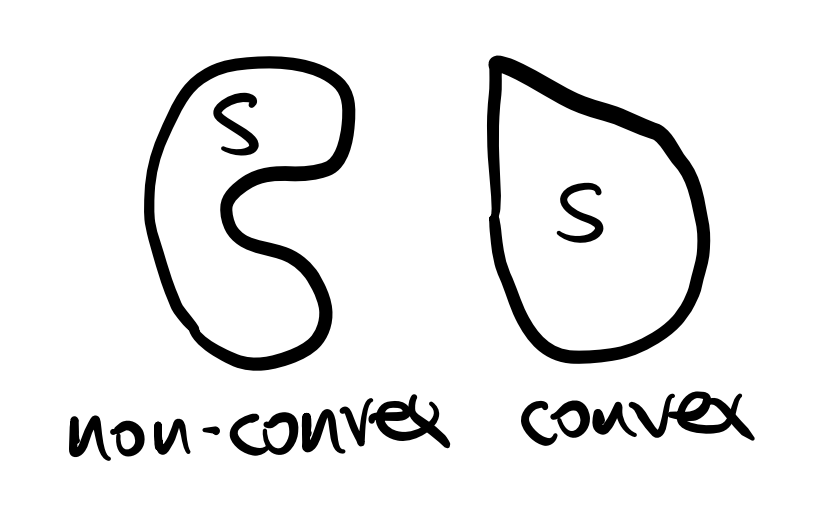
\includegraphics[width=4cm]{notes/figures/convex_set.png}
\caption{Sequential resistors.}\label{fig:sequential_resistors}
\end{marginfigure}
\begin{ex}
For the graph of \cref{fig:sequential_resistors}, $\Reff(1,k+1) = \sum_{i=1}^k \vr(i)$.
\end{ex}
\begin{proof}[Proof sketch] For the flow to be $1$, by Ohm's law, the voltage difference across edge $i$ must be $\vr(i)$.
\end{proof}

\begin{marginfigure}
TBD
% \centering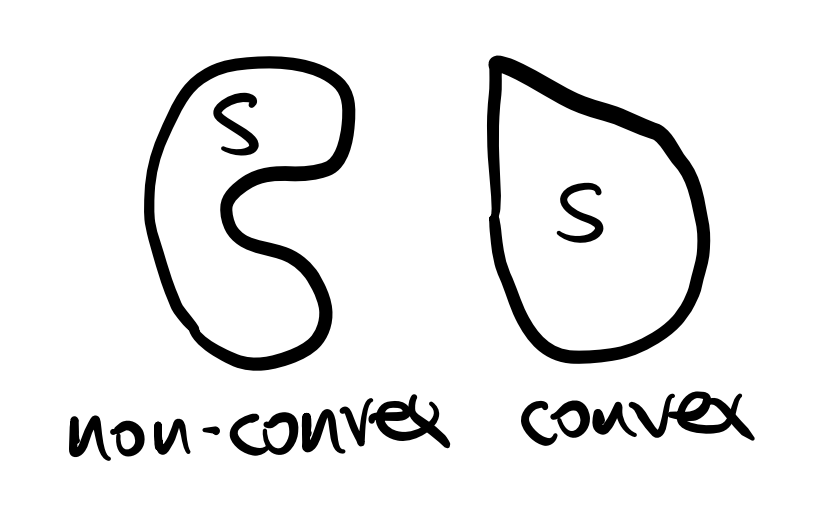
\includegraphics[width=4cm]{notes/figures/convex_set.png}
\caption{Parallel resistors.}\label{fig:parallel_resistors}
\end{marginfigure}
\begin{ex}
For the graph of \cref{fig:parallel_resistors}, $\Reff(1,2) = \frac{1}{\sum_{i=1}^k \nicefrac{1}{\vr(i)}}$.
\end{ex}
\begin{proof}[Proof sketch] For the flow to be $1$, by Ohm's law, we must have, \begin{align*}
    1 = \sum_{i=1}^k \frac{\elx(\{1,2\})}{\vr(i)},
\end{align*} where $\elx(\{1,2\})$ is the voltage difference between vertices $1$ and $2$. Note that $\Reff(1,2) = \elx(\{1,2\})$.
\end{proof}

\begin{lem}
$\Reff(a,b) = \norm{\mL^{\nicefrac{+}{2}}(\vOne_b - \vOne_a)}_2^2$.
\end{lem}
\begin{proof} As the electrical flow $\ef$ is energy-minimizing, we have that $\Reff(a,b) = \trans{\ef}\mR\ef$. Recall that by Ohm's law this flow corresponds to voltages $\elx$ solving $\mL\elx = \vOne_b - \vOne_a$, that is, $\elx = \pinv{\mL}(\vOne_b - \vOne_a)$. We obtain, \begin{align*}
    \Reff(a,b) = \trans{\ef}\mR\ef = \trans{\elx}\mL\elx &= \trans{(\vOne_b - \vOne_a)}\pinv{\mL}\mL\pinv{\mL}(\vOne_b - \vOne_a) \\
    &= \trans{(\vOne_b - \vOne_a)}\pinv{\mL}(\vOne_b - \vOne_a) \margintag{using that $\vOne_b - \vOne_a \perp \vOne$} \\
    &= \norm{\mL^{\nicefrac{+}{2}}(\vOne_b - \vOne_a)}_2^2. \qedhere
\end{align*}
\end{proof}

\begin{lem}
If $G$ is a $\phi$-expander, then \begin{align}
    \Reff(a,b) \leq 2\phi^{-2}\parentheses*{\frac{1}{\vd(b)} + \frac{1}{\vd(a)}}.
\end{align}
\end{lem}
\begin{proof}
By Cheeger's inequality, \begin{align*}
    \phi \leq \phi(G) \leq \sqrt{2 \lambda_2(\mN)} \implies \frac{\phi^2}{2} \leq \lambda_2(\mN).
\end{align*} By Courant-Fischer, we have that for any $\vy \perp \ker{\mN}$, \begin{align*}
    \frac{\phi^2}{2} \leq \lambda_2(\mN) \leq \frac{\trans{\vy}\mN\vy}{\trans{\vy}\vy} \implies \frac{\phi^2}{2}\trans{\vy}\vy \leq \trans{\vy}\mN\vy.
\end{align*} Equivalently, \begin{align*}
    \frac{\phi^2}{2}\mPi_\mN \preceq \mN, \margintag{using that $\mPi_\mN \vv = \vv$ for $\vv \perp \ker{\mN}$, and $\mPi_\mN \vv = 0$ if $\vv \in \ker\mN$}
\end{align*} where $\mPi_\mN$ is the projection orthogonal to the kernel of $\mN$. From this we conclude that \begin{align*}
    2\phi^{-2}\mPi_\mN = 2\phi^{-2}\pinv{\mPi_\mN} \succeq \pinv{\mN}, \margintag{using $\pinv{\mPi_\mN} = \mPi_\mN$}
\end{align*} as $\mA \succeq \mB$ implies $\pinv{\mA} \preceq \pinv{\mB}$ when $\ker\mA = \ker\mB$. By \cref{eq:pinv_calculation}, \begin{align}
    \pinv{\mN} = \pinv{(\mD^{-\nicefrac{1}{2}}\mL\mD^{-\nicefrac{1}{2}})} = \mPi_\mN\mD^{\nicefrac{1}{2}}\pinv{\mL}\mD^{\nicefrac{1}{2}}\mPi_\mN
\end{align} Therefore, for any $\vy \perp \ker\mN$, \begin{align*}
    2\phi^{-2}\trans{\vy}\vy \geq \trans{\vy}\pinv{\mN}\vy = \trans{\vy}\mD^{\nicefrac{1}{2}}\pinv{\mL}\mD^{\nicefrac{1}{2}}\vy.
\end{align*} Substituting $\vz \defeq \mD^{-\nicefrac{1}{2}}\vy$, we obtain, \begin{align*}
    2\phi^{-2}\trans{\vz}\inv{\mD}\vz \geq \trans{\vz}\pinv{\mL}\vz.
\end{align*} Finally, observe that for $\vz \defeq \vOne_b - \vOne_a$, we have that $\vy = \mD^{\nicefrac{1}{2}}(\vOne_b - \vOne_a) \perp \ker\mN$ as $\vOne_b - \vOne_a \perp \ker\mL$ and therefore,\footnote{We have for the kernel of the normalized Laplacian matrix, $\mN = \mD^{-\nicefrac{1}{2}}\mL\mD^{-\nicefrac{1}{2}}$, that $\ker\mN = \mD^{\nicefrac{1}{2}}\ker\mL = \vspan\{\mD^{\nicefrac{1}{2}}\vOne\}$.} \begin{align*}
    \Reff(a,b) = \trans{\vz}\pinv{\mL}\vz \leq 2\phi^{-2}\trans{\vz}\inv{\mD}\vz = 2\phi^{-2}\parentheses*{\frac{1}{\vd(b)} + \frac{1}{\vd(a)}}. &\qedhere
\end{align*}
\end{proof}

\begin{lem}
$\E{C_{a,b}} = \norm{\vd}_1 \Reff(a,b)$.
\end{lem}
\begin{proof} Recall that $\E{C_{a,b}} = \trans{(\vOne_a - \vOne_b)}\elx$ for a solution $\elx$ to $\mL\elx = \norm{\vd}_1 (\vOne_a - \vOne_b)$, that is, $\elx = \norm{\vd}_1\pinv{\mL}(\vOne_a - \vOne_b)$. Now, observe that, \begin{align*}
    \Reff(b,a) = \trans{(\vOne_a - \vOne_b)}\pinv{\mL}(\vOne_a - \vOne_b) = \frac{1}{\norm{\vd}_1}\trans{(\vOne_a - \vOne_b)}\elx.
\end{align*} Thus, $\E{C_{a,b}} = \norm{\vd}_1 \Reff(b,a)$. Using symmetry of the commute time, $\E{C_{a,b}} = \E{C_{b,a}} = \norm{\vd}_1 \Reff(a,b)$.
\end{proof}

\begin{cor}\label{cor:effective_resistance_symmetric}
Effective resistance is symmetric.
\end{cor}

\section{Effective Resistance as a Metric}

Before showing that effective resistance is a metric on the set of vertices, we consider the following lemma. We will write, \begin{align}
    \elx_{a,b} \defeq \pinv{\mL}(\vOne_b - \vOne_a),
\end{align} for the electrical voltages required to route one unit of current from $a$ to $b$.

\begin{lem}\label{lem:voltages_are_weighted_average}
If $\elx_{a,b}$ is a solution to $\mL\elx_{a,b} = \vOne_b - \vOne_a$, then we have for all $c \in \sV$ that $\elx_{a,b}(b) \geq \elx_{a,b}(c) \geq \elx_{a,b}(a)$.
\end{lem}
\begin{proof}[Proof sketch] Consider any $c \in \sV \setminus \{a,b\}$. Then, $(\mL\elx_{a,b})(c) = 0$. Thus, \begin{align*}
    \parentheses*{\sum_{v \sim c} \vw(\{v,c\})} \elx_{a,b}(c) - \parentheses*{\sum_{v \sim c} \vw(\{v,c\}) \elx_{a,b}(v)} = 0.
\end{align*} So, we have, \begin{align*}
    \elx_{a,b}(c) = \frac{\sum_{v \sim c} \vw(\{v,c\}) \elx_{a,b}(v)}{\sum_{v \sim c} \vw(\{v,c\})}.
\end{align*} In words, the electrical voltage of $c$ is a weighted average of the voltages of its neighbors. It follows that the voltages of $a$ and $b$ take the largest absolute values.
\end{proof}

\begin{defn}[Metric] A \emph{metric}\index{metric} on a set $\sS$ is a function $d : \sS \times \sS \to \R$ such that for any $a, b, c \in \sS$, \begin{enumerate}
    \item $d(a,b) = 0 \iff a = b$;
    \item $d(a,b) \geq 0$;
    \item $d(a,b) = d(b,a)$; and
    \item $d(a,b) \leq d(a,c) + d(c,b)$.
\end{enumerate}
\end{defn}
\begin{lem}
Effective resistance is a metric on $\sV$.
\end{lem}
\begin{proof} It is easy to check that properties (1) and (2) are satisfied. We have that property (3) is satisfied by \cref{cor:effective_resistance_symmetric}.

Let us therefore consider property (4), the triangle inequality. We have, \begin{align*}
    \elx_{a,b} = \pinv{\mL}(\vOne_b - \vOne_a) = \pinv{\mL}(\vOne_c - \vOne_a + \vOne_b - \vOne_c) = \elx_{a,c} + \elx_{c,b},
\end{align*} This we can use to rephrase the effective resistance, \begin{align*}
    \Reff(a,b) = \trans{(\vOne_b - \vOne_a)}\elx_{a,b} &= \trans{(\vOne_b - \vOne_a)}(\elx_{a,c} + \elx_{c,b}) \\
    &= \elx_{a,c}(b) - \elx_{a,c}(a) + \elx_{c,b}(b) - \elx_{c,b}(a) \\
    &\leq \elx_{a,c}(c) - \elx_{a,c}(a) + \elx_{c,b}(b) - \elx_{c,b}(c) \margintag{using \cref{lem:voltages_are_weighted_average}} \\
    &= \trans{(\vOne_c - \vOne_a)}\elx_{a,c} + \trans{(\vOne_b - \vOne_c)}\elx_{c,b} \\
    &= \Reff(a,c) + \Reff(c,b). \qedhere
\end{align*}
\end{proof}
    % !TeX root = ../main.tex
% Add the above to each chapter to make compiling the PDF easier in some editors.

\chapter{Spectral Graph Sparsification}

Many combinatorial graph algorithms perform better on sparse graphs. In this chapter, we will see that for any dense graph, we can find a sparse graph with approximately the same Laplacian matrix as measured by quadratic forms.

\begin{defn}[Matrix approximation]\index{matrix approximation} Given $\mA, \mB \in \sS_+^n$ and $\epsilon > 0$, we say, \begin{align}
    \mA \approx_\epsilon \mB \quad\text{iff}\quad \frac{1}{1+\epsilon}\mA \preceq \mB (1+\epsilon)\mA.
\end{align}
\end{defn}

Given some graph $G = (\sV,\sE,\vw)$, our goal is to find a graph $\Tilde{G} = (\sV,\Tilde{\sE},\Tilde{\vw})$ such that $|\Tilde{\sE}| \ll |\sE|$ and $\mL_G \approx_\epsilon \mL_{\Tilde{G}}$. We will write $\mL \defeq \mL_G$ and $\Tilde{\mL} \defeq \mL_{\Tilde{G}}$.

\begin{lem}
If $\mL \approx_\epsilon \Tilde{\mL}$, then for any cut $(\sS, \sV \setminus \sS)$, \begin{align}
    \frac{1}{1+\epsilon}c_G(\sS) \leq c_{\Tilde{G}}(\sS) \leq (1+\epsilon)c_G(\sS).
\end{align}
\end{lem}
\begin{proof}
Recall that $c_G(\sS) = \trans{\vOne_\sS}\mL\vOne_\sS$. The statement follows immediately by comparing the quadratic forms.
\end{proof}

\begin{thm}[Spectral graph approximation by sampling]
For any $\epsilon, \delta \in (0,1)$, there exist sampling probabilities $p_e$ for each edge $e \in \sE$ such that if $e \in \Tilde{\sE}$ with probability $p_e$ and $\Tilde{\vw}(e) \defeq \nicefrac{\vw(e)}{p_e}$, then with probability at least $1-\delta$ the graph $\Tilde{G} = (\sV,\Tilde{\sE},\Tilde{\vw})$ satisfies,\cite{spielman2011graph} \begin{align*}
    \mL \approx_\epsilon \Tilde{\mL} \quad\text{and}\quad |\Tilde{\sE}| = \LandauO{\frac{n}{\epsilon} \log\parentheses*{\frac{n}{\delta}}}.
\end{align*}
\end{thm}
\begin{proof}
TBD
\end{proof}
    % !TeX root = ../main.tex
% Add the above to each chapter to make compiling the PDF easier in some editors.

\chapter{Solving Laplacian Linear Systems}

    \part{Combinatorial Graph Algorithms}
    % !TeX root = ../main.tex
% Add the above to each chapter to make compiling the PDF easier in some editors.

\chapter{Algorithms for Maximum Flow}

In this chapter, we study classical combinatorial algorithms for the maximum flow problem. Many of the algorithms can be adapted to solve the more general minimum-cost flow problem. In recent years, we have made significant progress by using convex optimization and interior point methods.

We consider directed graphs $G = (V, E, \vc)$ with edge capacities $\vc \in \R^{|\sE|}$. Recall that a \emph{flow}\index{flow} is a vector $\vf \in \R^{|\sE|}$ and $\vf$ routes demands $\vd$ iff $\mB\vf = \vd$. We say that $\vf$ is \emph{feasible}\index{feasible flow} iff $\vZero \leq \vf \leq \vc$, where $\vZero \leq \vf$ ensures that the flow respects edge directions and $\vf \leq \vc$ ensures that the flow respects edge capacities.

We call a flow $\vf$ that routes demands $F(\vOne_t - \vOne_s)$ for some $F \in \R$ and vertices $s,t \in \sV$, so $F$ units of flow from $s$ to $t$, an \emph{$s$-$t$ flow}\index{s-t flow} with \emph{value}\index{flow value} $\val(\vf) = F$. We say that $\vf$ is \emph{optimal} iff there is no feasible $s$-$t$ flow $\vf'$ such that $\val(\vf') > \val(\vf)$.

We can decompose any $s$-$t$ flow into two kinds of flows: path flows and cycle flows.

\begin{defn}[Path flow]
An \emph{$s$-$t$ path flow}\index{$s$-$t$ path flow} $\vf$ is an $s$-$t$ flow with $\val(\vf) = \alpha$ for some $\alpha > 0$ that can be expressed as, \begin{align}
    \vf = \alpha\sum_{e \in \sP} \vOne_e,
\end{align} for some $s$-$t$ path $\sP$.
\end{defn}
\begin{marginfigure}
TBD
% \centering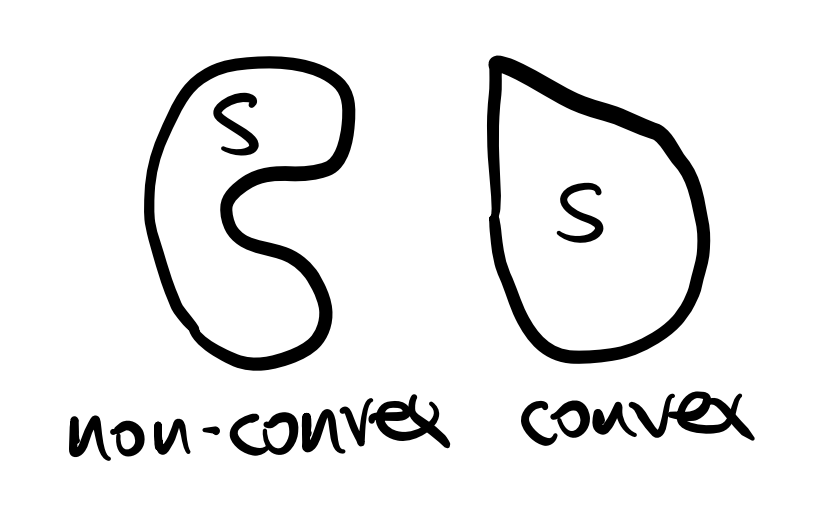
\includegraphics[width=4cm]{notes/figures/convex_set.png}
\caption{Example of an $s$-$t$ path flow.}
\end{marginfigure}
\begin{defn}[Cycle flow]
A \emph{cycle flow}\index{cycle flow} $\vf$ is a flow routing demands $\vZero$ that can be expressed as, \begin{align}
    \vf = \alpha\sum_{e\in\sC} \vOne_e,
\end{align} for some $\alpha > 0$, and cycle $\sC$.
\end{defn}
\begin{marginfigure}
TBD
% \centering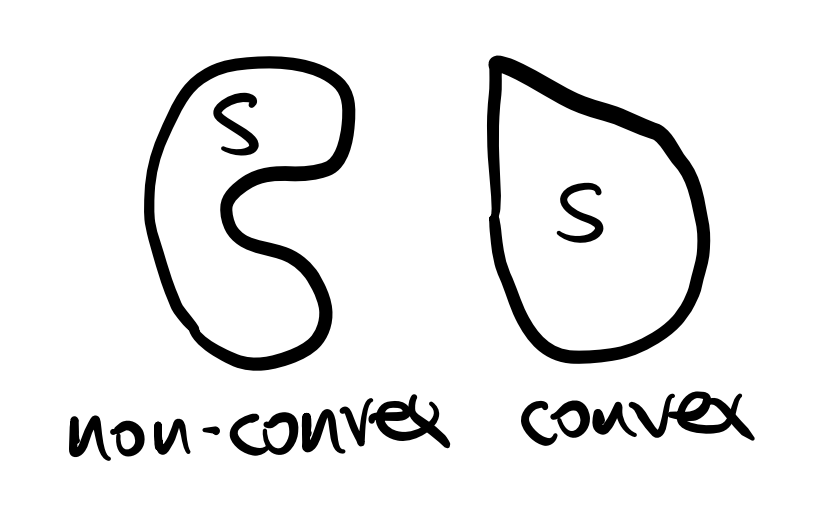
\includegraphics[width=4cm]{notes/figures/convex_set.png}
\caption{Example of a cycle flow.}
\end{marginfigure}
\begin{lem}[Path-cycle decomposition]
Any $s$-$t$ flow $\vf \geq \vZero$ can be decomposed into $k \leq m$ $s$-$t$ path flows and $l$ cycle flows.
\end{lem}
\begin{proof}
TBD
\end{proof}

\begin{lem}
There exists an optimal flow with a path-cycle decomposition that has only paths and no cycles.
\end{lem}
\begin{proof}
TBD
\end{proof}

\begin{lem}
There exists an $s$-$t$ flow $\vf \geq \vZero$ iff there exists a directed $s$-$t$ path.
\end{lem}
\begin{proof}
TBD
\end{proof}

Recall that a \emph{cut}\index{cut} is a proper subset of vertices $\emptyset \subset \sS \subset \sV$. An \emph{$s$-$t$ cut}\index{s-t cut} is a cut $(\sS, \sV \setminus \sS)$ separating $s$ and $t$, i.e., $s \in \sS, t \in \sV \setminus \sS$. We say that the capacity of a cut is the sum of capacities of crossing edges, \begin{align}
    \capa(\sS) \defeq \sum_{\substack{\{a,b\} \in \sE \\ a \in \sS,\ b \in \sV \setminus \sS}} \vc(\{a,b\}).
\end{align}

\begin{thm}[Weak duality of maximum flow/minimum cut]
For any feasible $s$-$t$ flow $\vf$ and any $s$-$t$ cut $(\sS, \sV \setminus \sS)$, \begin{align}
    \val(\vf) \leq \capa(\sS).
\end{align}
\end{thm}
\begin{proof}
Let $(\sS, \sV \setminus \sS)$ be any $s$-$t$ cut. Suppose for a contradiction that $\val(\vf) > \capa(\sS)$ for some flow $\vf$. But this contradicts feasibility of $\vf$ because the crossing edges of the cut form a bottleneck.
\end{proof}

An important concept in the analysis of flow algorithms is the so-called residual graph.

\begin{defn}[Residual graph]
The \emph{residual graph}\index{residual graph} $G_\vf$ of some $s$-$t$ flow $\vf \geq \vZero$ is the graph $G$ with edge capacities $[-\vf, \vc - \vf]$. That is, we say that a flow $\hat{\vf}$ is \emph{feasible} in the residual graph iff $-\vf \leq \hat{\vf} \leq \vc - \vf$.
\end{defn}

Intuitively, sending positive flow $\vc - \vf$ along an edge in $G_\vf$ corresponds to sending the maximum additional flow without violating the capacity constraint within $G$, whereas sending negative flow $-\vf$ along an edge in $G_\vf$ corresponds to ``undoing'' the flow that was send along this edge by $\vf$. This simple argument shows that if $\hat{\vf}$ is feasible in $G_\vf$, then $\vf + \hat{\vf}$ is feasible in $G$.

We call an $s$-$t$ flow $\hat{\vf}$ in $G_\vf$ an \emph{augmenting flow}\index{augmenting flow} of $\vf$.

\begin{lem}[Flow optimality condition]
A feasible $s$-$t$ flow $\vf$ in $G$ is optimal iff there is no $s$-$t$ path in $G_\vf$, or equivalently, iff there is no $\vf$-augmenting flow.
\end{lem}
\begin{proof}
TBD
\end{proof}

\begin{thm}[Strong duality of maximum flow/minimum cut]
We have that, \begin{align}
    \max_{\substack{F \in \R,\ \vf \in \R^{|\sE|} \\ \mB\vf = F(\vOne_t - \vOne_s)}} F = \min_{\text{$s$-$t$ cut $(\sS, \sV \setminus \sS)$}} \capa(\sS).
\end{align}
\end{thm}
\begin{proof}
By weak duality of maximum flow and minimum cut, we have the direction $\leq$. For the direction $\geq$, let $\s{\vf}$ be an optimal flow and consider the cut, \begin{align*}
    \sS \defeq \{v \in \sV \mid \text{there exists an $s$-$v$ path in $G_{\s{\vf}}$}\}.
\end{align*} We make two observations. \begin{enumerate}
    \item By definition, there are no edges from $\sS$ to $\sV \setminus \sS$ in $G_{\s{\vf}}$, that is, $\s{\vf}$ \emph{saturates}\footnote{That is, $\s{\vf}$ sends flow equal to the capacity of the edge.} all crossing edges of the cut.
    \item By definition, $\s{\vf}$ routes no flow from $\sV \setminus \sS$ to $\sS$.
\end{enumerate}\noindent This implies that $\val(\s{\vf}) \geq \capa(\sS)$ for this cut $(\sS, \sV \setminus \sS)$.
\end{proof}

\section{The Ford-Fulkerson Algorithm}

Our prior discussion gives rise to a very natural algorithm.

\begin{algorithm}
    \caption{\textsc{FordFulkerson($G$)}}\index{Ford-Fulkerson algorithm}
    $\vf \gets \vZero$\;
    \While{there exists any $s$-$t$ path flow $\hat{f}$ in $G_\vf$}{
        $\vf \gets \vf + \hat{\vf}$\;
    }
    \Return{$\vf$}
\end{algorithm}

Given a feasible flow $\vf$, we can find an $\vf$-augmenting flow, or determine that none exists, in time $\LandauO{m}$ using breadth-first search or depth-first search.

\begin{thm}[Ford-Fulkerson]
If capacities are integral, \textsc{FordFulkerson} converges to an optimal flow $\s{\vf}$ in $\val(\s{\vf})$ iterations.
\end{thm}
\begin{proof}
Observe that the initial flow $\vZero$ is trivially feasible. In each iteration, we add the augmenting flow $\hat{\vf}$ with $\val(\hat{\vf}) > 0$, and due to the integral capacities, $\val(\hat{\vf}) \geq 1$. Therefore, the flow value $\val(\vf)$ increases in each iteration by at least one.
\end{proof}

\subsection{Improving Ford-Fulkerson}

It turns out that if we always choose the shortest augmenting path, we converge in time $\LandauO{n m^2}$. This is known as the \emph{Edmonds-Karp algorithm}\index{Edmonds-Karp algorithm}.

We can do still better, by choosing that path with the maximum bottleneck capacity. That is, we choose, \begin{align}
    \s{\sP} = \argmax_{\text{augmenting paths $\sP$}} \min_{e \in \sP} \vc(e).
\end{align} Within the framework of Ford-Fulkerson this corresponds to the augmenting path that allows us to route the most additional flow.

\begin{thm}
\textsc{FordFulkerson}, where in each iteration we choose the augmenting path with maximum bottleneck capacity, converges in time $\LandauO{m^2 \log mU}$.
\end{thm}
\begin{proof}
We can find $\s{\sP}$ using a binary search on $[1,U]$, where $U \defeq \max_e \vc(e)$, by removing all edges with absolute capacity in $G_\vf$ below the current threshold and testing if an $s$-$t$ path in $G_\vf$ exists: if it does, we increase the threshold; if it does not, we decrease the threshold. This procedure takes $\LandauO{m \log U}$ time. If we only consider the occurring capacities, the runtime improves to $\LandauO{m \log m}$.

Suppose $\hat{F}$ is the flow left in $G_\vf$. By the path decomposition lemma, this flow can be decomposed into at most $m$ path flows (the ``best'' of which is $\s{\sP}$) and $\s{\sP}$ must route at least the average amount of flow. Hence, $\s{\sP}$ routes at least $\nicefrac{\hat{F}}{m}$ units of flow. Thus, the algorithm converged if, \begin{align*}
    \parentheses*{1 - \frac{1}{m}}^T \s{F} < 1,
\end{align*} where $T$ is the number of augmentations and $\s{F}$ is the value of an optimal flow. So, some $T = \LandauO{m \log \s{F}}$ is sufficient.

Overall, we get, \begin{align*}
    \LandauO{m \log m \cdot T} = \LandauO{m^2 \log (m+\s{F})} = \LandauO{m^2 \log mU} \margintag{using $\s{F} \leq mU$} &\qedhere
\end{align*}
\end{proof}

\section{Dinitz's Algorithm}

We will now look at Dinitz's algorithm, which also belongs to the family of Ford-Folkerson algorithms. That is, we still start with the initial feasible flow $\vf \gets \vZero$ and iteratively improve this flow by finding an augmenting flow in $G_\vf$.

In Dinitz's algorithm, our strategy to finding an augmenting path is to find so-called \emph{blocking flows} in $G_\vf$, which in each iteration ``block'' one shortest $s$-$t$ path in $G_\vf$. Dinitz's algorithm runs in $\LandauO{n^2 + nm \log^2 n}$ time in general graphs and in time $\LandauO{\min\{m^{\nicefrac{3}{2}}, m n^{\nicefrac{2}{3}}\}}$ in unit capacity graphs.

\begin{rmk}
It can also be shown that Dinitz's algorithm converges in time $\LandauO{m \sqrt{n}}$ in bipartite matching graphs, but we will not show this here.
\end{rmk}

\begin{defn}[Level]
The \emph{level}\index{level} $\ell(v)$ of a vertex $v \in \sV$ in $G_\vf$ is the length (i.e., number of edges) of the shortest $s$-$v$ path in $G_\vf$.

We call an edge $e = (u,v)$ in $G_\vf$ \emph{admissible} iff $\ell(v) = \ell(u)+1$. Intuitively, $e$ is admissible iff it is part of a shortest $s$-$u$ path.

The \emph{level graph}\index{level graph} $L_\vf$ of $G_\vf$ is the subgraph of only admissible edges.
\end{defn}
\begin{marginfigure}
TBD
% \centering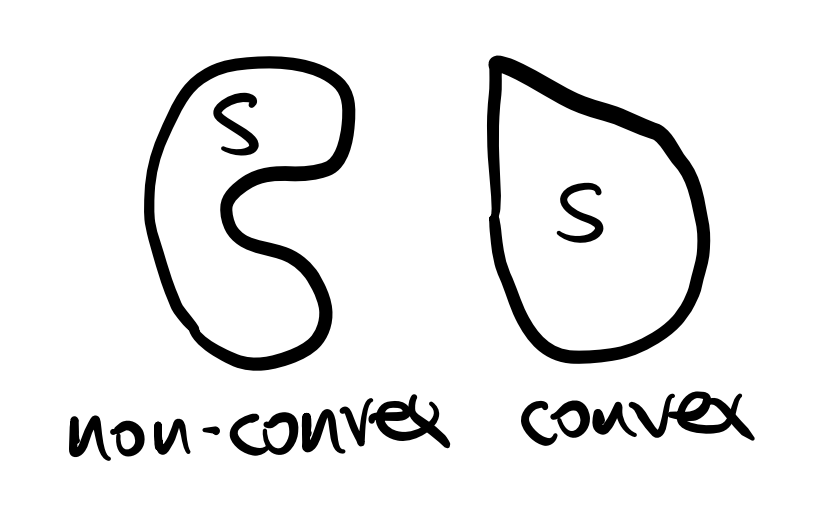
\includegraphics[width=4cm]{notes/figures/convex_set.png}
\caption{Illustration of admissible edges.}
\end{marginfigure}

\begin{defn}[Blocking flow]
A \emph{blocking flow}\index{blocking flow} in $G_\vf$ is a flow $\hat{\vf}$ such that \begin{enumerate}
    \item $\hat{\vf}$ is feasible;
    \item $\hat{\vf}$ uses only admissible edges; and
    \item for every $s$-$t$ path in the level graph, $\hat{\vf}$ saturates at least one edge.
\end{enumerate}
\end{defn}
\begin{rmk}
By definition, a blocking flow in $G_\vf$ is a $\vf$-augmenting flow.
\end{rmk}
\begin{marginfigure}
TBD
% \centering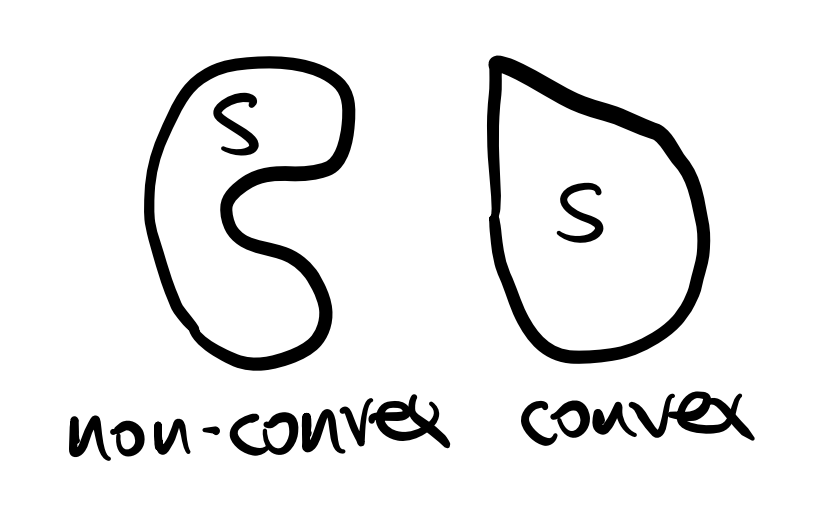
\includegraphics[width=4cm]{notes/figures/convex_set.png}
\caption{Examples of blocking flows.}
\end{marginfigure}

\begin{algorithm}
    \caption{\textsc{Dinitz($G$)}}\index{Dinitz's algorithm}
    $\vf \gets \vZero$\;
    \Repeat{$G_\vf$ is disconnected}{
        $\hat{\vf} \gets \text{blocking flow in $G_\vf$}$\;
        $\vf \gets \vf + \hat{\vf}$\;
    }
    \Return{$\vf$}
\end{algorithm}

\begin{lem}
Let $\vf$ be a feasible flow, $\hat{\vf}$ a blocking flow in $G_\vf$, and let $\vf' \defeq \vf + \hat{\vf}$. Then $\ell_{G_{\vf'}}(t) > \ell_{G_\vf}(t)$.
\end{lem}
\begin{proof}
TBD
\end{proof}

\begin{thm}[Dinitz]
Dinitz's algorithm converges in $\LandauO{n}$ iterations.
\end{thm}
\begin{proof}
By the previous lemma, $\ell(t)$ increases in every iteration by at least one. As path can contain each vertex at most once, the level of any vertex can never be larger than $n$.
\end{proof}

\subsection{Finding Blocking Flows}

A naïve approach is to repeatedly use depth-first search to find an unsaturated $s$-$t$ path in the level graph $L_\vf$. Whenever we find such a path, we route the maximum possible flow along this path, saturating at least one of its edges.

\begin{algorithm}
    \caption{\textsc{FindBlockingFlow($L_\vf$)}}
    $\hat{\vf} \gets \vZero$\;
    \While{there exists an $s$-$t$ path $\sP$ in $L_\vf$}{
        Let $\hat{\vf}'$ be a flow saturating $\sP$\;
        $\hat{\vf} \gets \hat{\vf} + \hat{\vf}'$\;
        Remove all edges saturated by $\hat{\vf}'$ from $L_\vf$\;
    }
    \Return{$\hat{\vf}$}
\end{algorithm}

\begin{lem}
\textsc{FindBlockingFlow} returns a blocking flow in $\LandauO{mn}$ time.
\end{lem}
\begin{rmk}
This can be improved to $\LandauO{m \log^2 n + n}$ by using link-cut trees, which we will discuss in the next chapter.
\end{rmk}
\begin{proof}
TBD
\end{proof}

\subsection{Unit Capacity Graphs}

\begin{lem}
In unit capacity graphs, \textsc{FindBlockingFlow} returns a blocking flow in $\LandauO{m}$ time.
\end{lem}
\begin{proof}
TBD
\end{proof}

\begin{thm}
In unit capacity graphs, Dinic's algorithm terminates in $\LandauO{\min\{m^{\nicefrac{1}{2}}, n^{\nicefrac{2}{3}}\}}$ time.
\end{thm}
\begin{proof}
TBD
\end{proof}

\section{The Push-Relabel Algorithm}
% TBD

\section{Outlook}

We have seen two approaches to solving maximum flow problems: Ford-Fulkerson maintains a feasible flow and augments this flow until it is optimal. In contrast, Push-Relabel maintains that there is no augmenting path and terminates when the flow is feasible.

Currently, the best known algorithm for real-valued capacities is due to Orlin and takes $\LandauO{mn}$ time.\cite{orlin2013max}

Geometrically speaking, Ford-Fulkerson is analogous to a simplex method and Push-Relabel is analogous to an exterior-point method. In recent years, interior-point methods were used to find efficient algorithms when capacities are integral, the best known algorithm taking $\LandauO{m^{1+o(1)} \log U}$ time.\cite{chen2022maximum}
    % !TeX root = ../main.tex
% Add the above to each chapter to make compiling the PDF easier in some editors.

\chapter{Link-Cut Trees}
    % !TeX root = ../main.tex
% Add the above to each chapter to make compiling the PDF easier in some editors.

\chapter{Distance Oracles}

    \part{Further Topics}
    % !TeX root = ../main.tex
% Add the above to each chapter to make compiling the PDF easier in some editors.

\chapter{Finding Expanders using Maximum Flow}\label{cha:expanders_using_max_flow}

\section{Graph Embedding}
    % !TeX root = ../main.tex
% Add the above to each chapter to make compiling the PDF easier in some editors.

\chapter{Interior Point Methods for Maximum Flow}
    
    \appendix
    % !TeX root = ../main.tex
% Add the above to each chapter to make compiling the PDF easier in some editors.

\chapter{Solutions}

\section{\Cref{part1}}

\subsection{Electrical Flows}

\begin{proof}[Solution to \cref{exc:graph_laplacian_characterization}] TBD
\end{proof}

\begin{proof}[Proof of \cref{clm:electrical_flow_optimization_convex}] We have that $\mH_c(\vx) = \mL(\vx) \succeq \mZero$.
\end{proof}

\begin{proof}[Solution to \cref{exc:electrical_flow_energy_minimizing}] Consider any $\vf \in \R^{|\sE|}$ satisfying $\mB\vf = \vd$. We have for any $\vx \in \R^{|\sV|}$, \begin{align*}
    \frac{1}{2}\trans{\vf}\mR\vf &= \frac{1}{2}\trans{\vf}\mR\vf - \trans{\vx}\underbrace{(\mB\vf - \vd)}_{0} \\
    &\geq \min_{\vf' \in \R^{|\sE|}} \underbrace{\frac{1}{2}\trans{\vf'}\mR\vf' - \trans{\vx}(\mB\vf' - \vd)}_{\eqdef g(\vf')}.
\end{align*} Note that $g$ is convex. Taking the gradient gives, \begin{align*}
    \grad_{\vf'} g(\vf') = \mR\vf' - \trans{\mB}\vx.
\end{align*} So $\vf' = \inv{\mR}\trans{\mB}\vx$ is the minimizer of $g$. We obtain, \begin{align*}
    \frac{1}{2}\trans{\vf}\mR\vf \geq -\frac{1}{2}\trans{\vx}\mL\vx + \trans{\vd}\vx,
\end{align*} but $\trans{\Tilde{\vf}}\mR\Tilde{\vf} = \trans{\Tilde{\vx}}\mL\Tilde{\vx} = \trans{\vd}\Tilde{\vx}$ for electrical voltages $\Tilde{\vx}$ and electrical flow $\Tilde{\vf}$ (see \cref{eq:electrical_energy_demands}). Thus, \begin{align*}
    \frac{1}{2}\trans{\vf}\mR\vf \geq \frac{1}{2}\trans{\Tilde{\vx}}\mL\Tilde{\vx} = \frac{1}{2}\trans{\Tilde{\vf}}\mR\Tilde{\vf}.
\end{align*} Hence, $\Tilde{\vf}$ is the minimum electrical energy flow among all flows routing $\vd$.
\end{proof}

\begin{proof}[Solution to \cref{exc:electrical_energy_strong_duality}] TBD
\end{proof}

\begin{proof}[Solution to \cref{exc:electrical_energy_weak_duality}] TBD
\end{proof}

\subsection{Linear Algebra}

\begin{proof}[Proof of \cref{clm:eigenvalues_eigenvectors_of_matrix}] Because the characteristic polynomial of $\mA$ is of degree $n$, it has $n$ complex roots, which are the eigenvalues $\lambda_1, \dots, \lambda_n$ of $\mA$. We will first prove that the $\lambda_i$ are real. Then, we will prove that the corresponding eigenvectors $\vv_i$ are orthogonal.

\begin{enumerate}
    \item Let $\lambda$ be any eigenvalue of $\mA$. We denote by $\Bar{\lambda}$ the complex conjugate of $\lambda$. Clearly, if $\lambda = \Bar{\lambda}$, then $\lambda \in \R$. By the definition of the eigenvalue $\lambda$ with associated eigenvector $\vv$, we have, \begin{align*}
        \lambda\trans{\Bar{\vv}}\vv = \trans{\Bar{\vv}}\mA\vv.
    \end{align*} Taking the complex conjugate and transpose of both sides gives, \begin{align*}
        \Bar{\lambda}\trans{\Bar{\vv}}\vv = \trans{\Bar{\vv}}\trans{\Bar{\mA}}\vv = \trans{\Bar{\vv}}\mA\vv = \lambda\trans{\Bar{\vv}}\vv. \margintag{using that $\mA$ is real and symmetric, $\trans{\Bar{\mA}} = \mA$}
    \end{align*} We have $\lambda = \Bar{\lambda}$ as desired.
    
    \item It remains to show that for eigenvalues $\lambda_i, \lambda_j$ with associated eigenvectors $\vv_i, \vv_j$ and $i \neq j$, we have $\trans{\vv_i}\vv_j = 0$. By the definition of an eigenvalue, we have, \begin{align*}
        \lambda_i\trans{\vv_j}\vv_i = \trans{\vv_j}\mA\vv_i &= \trans{(\trans{\vv_i}\trans{\mA}\vv_j)} \\ &= \trans{(\trans{\vv_i}\mA\vv_j)} = \lambda_j \trans{(\trans{\vv_i}\vv_j)} = \lambda_j\trans{\vv_j}\vv_i. \margintag{using that $\mA$ is symmetric}
    \end{align*} We get that $\trans{\vv_j}\vv_i = 0$ if $\lambda_i \neq \lambda_j$. \qedhere
\end{enumerate}
\end{proof}

\begin{proof}[Proof of \cref{clm:eigenvalues_of_matrix_product}]
Suppose $\lambda$ is an eigenvalue of $\mM$ with associated eigenvector $\vv$. Also suppose that $\mT\vv = \vw$. Then, \begin{align*}
    \mT\mM\inv{\mT}\vw = \mT\mM\vv = \lambda\mT\vv = \vw.
\end{align*} It is easy to check that the other direction holds too.
\end{proof}

\begin{proof}[Proof of \cref{clm:matrix_function_facts}] TBD
\end{proof}

\begin{proof}[Proof of \cref{clm:orthogonal_projection}] TBD
\end{proof}

\begin{proof}[Proof of \cref{clm:pinv_calculation}] TBD
\end{proof}

\subsection{Probability}

\begin{thm}[Jensen's inequality, finite form]\label{thm:jensens_inequality_finite_form}
Let $f: \sS \to \R$ be a convex function on the convex set $\sS \subseteq \R^n$. Suppose that $\vx_1, \dots, \vx_k \sS$ and $\theta_1, \dots, \theta_k \geq 0$ with $\theta_1 + \dots + \theta_k = 1$. Then, \begin{align}
    f(\theta_1\vx_1 + \dots + \theta_k\vx_k) \leq \theta_1 f(\vx_1) + \dots + \theta_k f(\vx_k).
\end{align}
\end{thm}
\begin{proof}
We prove the statement by induction on $k$. The base case, $k = 2$, follows trivially from the convexity of $f$. For the induction step, suppose that the statement holds for some $k \geq 2$. Assume w.l.o.g. that $\theta_{k+1} \in (0,1)$. We have, \begin{align*}
    \sum_{i=1}^{k+1} \theta_i f(\vx_i) &= (1-\theta_{k+1})\parentheses*{\sum_{i=1}^k \frac{\theta_i}{1 - \theta_{k+1}} f(\vx_i)} + \theta_{k+1} f(\vx_{k+1}) \\
    &\geq (1-\theta_{k+1})f\parentheses*{\sum_{i=1}^k \frac{\theta_i}{1-\theta_{k+1}}\vx_i} + \theta_{k+1}f(\vx_{k+1}) \margintag{using the induction hypothesis} \\
    &\geq f\parentheses*{\sum_{i=1}^{k+1} \theta_i \vx_i}. \margintag{using convexity of $f$} &\qedhere
\end{align*}
\end{proof}

\section{\Cref{part2}}

\subsection{Convex Geometry}

\begin{proof}[Proof of \cref{thm:extreme_value_theorem}] In our proof, we will use the following two theorems.
\begin{fct}[Bolzano-Weierstrass theorem]\index{Bolzano-Weierstrass theorem} Every bounded sequence in $\R^n$ has a convergent subsequence.
\end{fct}
\begin{fct}[Boundedness theorem]\index{Boundedness theorem}
Let $f : \R^n \to \R$ be a continuous function and $\spa{F} \subseteq \R^n$ be non-empty, bounded, and closed. Then $f$ is bounded on $\spa{F}$.
\end{fct}

Let $\alpha$ be the infimum of $f$ over $\spa{F}$, i.e., the largest value for which any $\vx \in \spa{F}$ satisfies $f(\vx) \geq \alpha$. By the boundedness theorem, the infumum exists, as $f$ is lower bounded and the set of lower bounds has a greatest lower bound, $\alpha$.

Let $\spa{F}_k \defeq \{\vx \in \spa{F} \mid \alpha \leq f(\vx) \leq \alpha + 2^{-k}\}$. $\spa{F}_k$ cannot be empty, since if it were, then $\alpha + 2^{-k}$ would be a strictly greater lower bound on $f$ than $\alpha$. For each $k$, let $\vx_k$ be some $\vx \in \spa{F}_k$. $\{\vx_k\}_{k=1}^\infty$ is a bounded sequence as $\spa{F}_k \subseteq \spa{F}$, so by the Bolzano-Weierstrass theorem, there exists a convergent subsequence, $\{\vy_k\}_{k=1}^\infty$, with limit $\Bar{\vy}$. Because the set is closed, $\Bar{\vy} \in \spa{F}$. By continuity, $f(\Bar{\vy}) = \lim_{k\to\infty} f(\vy_k)$, and by construction, $\lim_{k\to\infty} f(\vy_k) = \alpha$.

Thus, the optimal solution is $\Bar{\vy}$.
\end{proof}

\begin{proof}[Solution to \cref{exc:convex_iff_epi_convex}] TBD
\end{proof}

\begin{proof}[Solution to \cref{exc:sub_level_set_of_convex_function_convex}] TBD
\end{proof}

\section{\Cref{part3}}

\subsection{Introduction to Spectral Graph Theory}

\begin{proof}[Solution to \cref{exc:spectrum_path_graph_2}] TBD
\end{proof}

\begin{proof}[Solution to \cref{exc:spectrum_path_graph_n}] TBD
\end{proof}

\begin{proof}[Solution to \cref{exc:spectrum_complete_binary_tree_2}] TBD
\end{proof}

\begin{proof}[Solution to \cref{exc:spectrum_complete_binary_tree_n}] TBD
\end{proof}

\subsection{Conductance and Expanders}

\begin{proof}[Solution to \cref{exc:expander_complete_graph}] TBD
\end{proof}

\begin{proof}[Solution to \cref{exc:expander_path_graph}] TBD
\end{proof}

    \backmatter

    % !TeX root = ../main.tex
% Add the above to each chapter to make compiling the PDF easier in some editors.

\chapter{Summary of Notation}

\begin{fullwidth}
We follow these general rules: \begin{itemize}[noitemsep]
    \item uppercase italic for constants $N$
    \item lowercase italic for indices $i$ and scalar variables $x$
    \item lowercase italic bold for vectors $\vx$
    \item uppercase italic bold for matrices $\mM$
    \item uppercase italic for random variables $X$
    \item uppercase bold for random vectors $\rX$
    \item uppercase italic for sets $\sA$
    % \item uppercase calligraphy for spaces (usually infinite sets) $\spA$
\end{itemize}

\begin{longtable}{p{2.5cm}l}
   $\defeq$ & equality by definition \\
   iff & if and only if \\
%   $\approx$ & approximately equals \\
%   $\propto$ & proportional to \\
   $\Nat$ & set of natural numbers $\{1, 2, \dots\}$ \\
   $\Nat_0$ & set of natural numbers, including $0$, $\Nat \cup \{0\}$ \\
   $\R$ & set of real numbers \\
   $\C$ & set of complex numbers \\
   $[m]$ & set of natural numbers from $1$ to $m$, $\{1, 2, \dots, m-1, m\}$ \\
%   $i:j$ & subset of natural numbers between $i$ and $j$, $\{i, i+1, \dots, j-1, j\}$ \\
   $(a,b]$ & real interval between $a$ and $b$ including $b$ but not including $a$ \\
   $f : \sA \to : \sB$ & function $f$ from elements of set $\sA$ to elements of set $\sB$ \\
   $\Ind{predicate}$ & indicator function ($\Ind{predicate} \defeq 1$ if the $predicate$ is true, else $0$) \\
   $\gets$ & assignment \\
\end{longtable}

\vspace{0cm}\section*{\smallcaps{Linear Algebra}}\vspace{-0.5cm}
\begin{longtable}{p{2.5cm}l}
   $\sS^n$ & set of symmetric $n \times n$ matrices \\
   $\sS_+^n$ & set of symmetric and positive semi-definite $n \times n$ matrices \\
   $\sS_{++}^n$ & set of symmetric and positive definite $n \times n$ matrices \\
   $\mA \preceq \mB$ & Loewner order on symmetric matrices, $\forall \vx \in \R^n: \trans{\vx}\mA\vx \leq \trans{\vx}\mB\vx$ \\
   \addlinespace
   $\vx \perp \vy$ & $\vx$ and $\vy$ are orthogonal, i.e., $\trans{\vx}\vy = 0$ \\
   $\vx \perp \sW$ & $\vx$ is orthogonal to every vector $\vy$ in subspace $\sW$ \\
   $\compl{\sW}$ & orthogonal complement of subspace $\sW$, $\{\vx \in \R^n \mid \vx \perp \sW\}$ \\
   $\vspan\{\vx_1, \dots, \vx_n\}$ & smallest subspace containing $\vx_1, \dots, \vx_n$ \\
   $\dim(\sW)$ & number of vectors in a basis of a subspace $\sW$ \\
   \addlinespace
   $\vOne_\sS$ & vector such that $\vOne_\sS(i) = \Ind{i \in \sS}$ \\
   $\trans{\mA}$ & transpose of matrix $\mA$ \\
   $\inv{\mA}$ & inverse of matrix $\mA$ \\
   $\pinv{\mA}$ & pseudoinverse of matrix $\mA$ \\
   $\mA^{\nicefrac{1}{2}}$ & square root of symmetric positive semi-definite matrix $\mA$ \\
   $\mPi_\mA$ & orthogonal projection to $\compl{(\ker{\mA})}$ \\
   \addlinespace
   $\nnz{\mA}$ & number of non-zero entries of $\mA$ \\
   $\tr{\mA}$ & trace of $\mA$, $\sum_i \mA(i,i)$ \\
   $\diag_{i\in\sI}\{a_i\}$ & diagonal matrix with elements $a_i$, indexed according to the set $\sI$ \\
   $\ker\mA$ & kernel (or null space) of $\mA$, $\{\vx \in \R^n \mid \mA\vx = \vZero\}$ \\
   $\im\mA$ & image of $\mA$, $\vspan\{\mA(:,i)\}_{i\in[n]}$ \\
   $\lambda_i(\mA)$ & $i$-th smallest eigenvalue of $\mA$ \\
   $\norm{\mA}_{\alpha\to\beta}$ & matrix norm of $\mA$ induced by norms $\norm{\cdot}_\alpha$ and $\norm{\cdot}_\beta$ \\
\end{longtable}

\vspace{0.5cm}\section*{\smallcaps{Probability}}\vspace{-0.5cm}
\begin{longtable}{p{2.5cm}l}
   $\Pr{X = x}$ & probability of a random variable $X$ taking on the value $x$ \\
   $X \sim F$ & random variable $X$ follows the distribution $F$ \\
   $x \sim F$ & value $x$ is sampled according to distribution $F$ \\
  $X \perp Y$ & random variable $X$ is independent of random variable $Y$ \\
  $X \perp Y \mid Z$ & \makecell[tl]{random variable $X$ is conditionally independent of random variable $Y$ \\ given random variable $Z$} \\
   $\E{X}$ & expected value of random variable $X$ \\
%   $\E[x \sim X]{f(x)}$ & expected value of the random variable $f(X)$, $\E{f(X)}$ \\
  $\Var{X}$ & variance of random variable $X$ \\
%   $\Cov{X,Y}$ & covariance of random variable $X$ and random variable $Y$ \\
%   $\Delta^{\spA}$ & set of all probability distributions over the set $\spA$ \\
    \addlinespace
   $\mW \in \R^{|\sV|\times|\sV|}$ & transition matrix of random walk, $\mA\inv{\mD} = \mI - \mD^{\nicefrac{1}{2}}\mN\mD^{-\nicefrac{1}{2}}$ \\
   $\Tilde{\mW} \in \R^{|\sV|\times|\sV|}$ & transition matrix of lazy random walk, $\frac{\mI}{2} + \frac{\mW}{2} = \mI - \frac{1}{2}\mD^{\nicefrac{1}{2}}\mN\mD^{-\nicefrac{1}{2}}$ \\
   $\vp_t \in \R^{|\sV|}$ & probability distribution of a random walk at time $t$, $\mW^t\vp_0$ \\
\end{longtable}

\vspace{0.5cm}\section*{\smallcaps{Analysis}}\vspace{-0.5cm}
\begin{longtable}{p{2.5cm}l}
   $\grad f(\vx) \in \R^{n \times 1}$ & gradient of a function $f$ at a point $\vx$, $\trans{\begin{bmatrix}
        \pdv{f(\vx)}{\vx(1)} & \cdots & \pdv{f(\vx)}{\vx(n)}
    \end{bmatrix}}$ \\
   $[\vx,\vy]$ & set of convex combinations of $\vx$ and $\vy$, $\{\theta\vx + (1-\theta)\vy \mid \theta\in[0,1]\}$ \\
   $D f(\vx)[\vd]$ & directional derivative of $f$ at $\vx$ in direction $\vd$, $\lim_{\lambda \to 0} \frac{f(\vx + \lambda\vd) - f(\vx)}{\lambda}$ \\
   $D \vg(\vx) \in \R^{m \times n}$ & Jacobian of vector-valued function $\vg: \R^n \to \R^m$, $\begin{bmatrix}
        \pdv{\vg(\vx)}{\vx(1)} & \cdots & \pdv{\vg(\vx)}{\vx(n)}
    \end{bmatrix}$ \\
   $\mH_f(\vx) \in \R^{n \times n}$ & Hessian of $f$, $\trans{(D \grad f(\vx))}$ \\
   \addlinespace
   $\mathrm{epi}(f)$ & epigraph of a function $f$, $\{(\vx,y) \mid f(\vx) \leq y\} \subseteq \R^{n+1}$ \\
   $\sS_\alpha(f)$ & $\alpha$-sub-level set of a function $f$, $\{\vx \in \sS \mid f(\vx) \leq \alpha\}$ \\
   $\sL_\alpha(f)$ & $\alpha$-level set of a function $f$, $\{\vx \in \sS \mid f(\vx) = \alpha\}$ \\
\end{longtable}

\vspace{0.5cm}\section*{\smallcaps{Graphs}}\vspace{-0.5cm}
\begin{longtable}{p{2.5cm}l}
   $\sV$ & set of vertices \\
   $\sE$ & set of edges \\
   $G[\sX]$ & subgraph of $G$ induced by $\sX \subseteq \sV$ \\
   $u \sim v$ & vertices $u$ and $v$ are adjacent \\
   $\deg(v)$ & degree of vertex $v$ \\
   \addlinespace
   $\vr \in \R^{|\sE|}$ & resistances \\
   $\vw \in \R^{|\sE|}$ & weights, $\nicefrac{1}{\vr(e)}$ \\
   $\vd \in \R^{|\sV|}$ & weighted degrees, $\sum_{\{u,v\} \in \sE} \vw(\{u,v\})$ \\
   $\Tilde{\mA} \in \R^{|\sV|\times|\sV|}$ & adjacency matrix \\
   $\mA \in \R^{|\sV|\times|\sV|}$ & weighted adjacency matrix \\
   $\mB \in \R^{|\sV|\times|\sE|}$ & incidence matrix \\
   $\mR \in \R^{|\sE|\times|\sE|}$ & diagonal matrix of resistances, $\diag\{\vr(e)\}_{e \in \sE}$ \\
   $\mW \in \R^{|\sE|\times|\sE|}$ & diagonal matrix of weights, $\diag\{\vw(e)\}_{e \in \sE}$ \\
   $\mD \in \R^{|\sV|\times|\sV|}$ & diagonal matrix of weighted degrees, $\diag\{\vw(v)\}_{v \in \sV}$ \\
   $\mL \in \R^{|\sV|\times|\sV|}$ & Laplacian matrix, $\mB\mR^{-1}\trans{\mB} = \mB\mW\trans{\mB} = \mD - \mA$ \\
   \addlinespace
   $\vol(\sS)$ & volume of a set of vertices $\sS$, $\sum_{v \in \sS} \vd(v) = \trans{\vOne_\sS}\mD\vOne_\sS$ \\
   $c(\sS)$ & value of a cut $\sS$, $\sum_{\{a,b\} \in \sE:\ a \in \sS,\ b \in \sV \setminus \sS} \vw(\{a,b\}) = \trans{\vOne_\sS}\mL\vOne_\sS$ \\
   $\phi(\sS)$ & conductance of a cut $\sS$, $\frac{c(\sS)}{\min\{\vol(\sS), \vol(\sV \setminus \sS)\}}$ \\
   $\phi(G)$ & conductance of a graph $G$, $\min_{\emptyset \subset \sS \subset \sV} \phi(S)$ \\
   $\sigma(\sS)$ & sparsity of a cut $\sS$, $\frac{c(\sS)}{\min\{|\sS|, |\sV \setminus \sS|\}}$ \\
   $\sigma(G)$ & sparsity of a graph $G$, $\min_{\emptyset \subset \sS \subset \sV} \sigma(S)$ \\
   \addlinespace
   $K_n$ & unit weight complete graph on $n$ vertices \\
   $P_n$ & unit weight path graph on $n$ vertices \\
   $T_d$ & unit weight complete binary tree with $d$ levels \\
   $G_{i,j}$ & unit weight graph with single edge $\{i,j\}$ \\
   $G^{i,j}$ & subgraph of $G$ consisting of the shortest $i,j$ path \\
\end{longtable}

\vspace{0.5cm}\section*{\smallcaps{Flows}}\vspace{-0.5cm}
\begin{longtable}{p{2.5cm}l}
   $\vx \in \R^{|\sV|}$ & voltages \\
   $\vx(e)$ & voltage difference of edge $e = \{u,v\}$, $\vx(u) - \vx(v)$ \\
   $\vf \in \R^{|\sE|}$ & flow \\
   $\vd \in \R^{|\sV|}$ & demands, modeling the net flow \\
   \addlinespace
   $\ex \in \R^{|\sV|}$ & electrical voltages \\
   $\ex_{a,b} \in \R^{|\sV|}$ & electrical voltages routing demands $\vOne_b - \vOne_a$ \\
   $\ef \in \R^{|\sE|}$ & electrical flow \\
   $\e(\ef), \e(\ex), \e(\vd)$ & electrical energy, $\trans{\ef}\trans{\mB}\ex = \trans{\ef}\mR\ef = \trans{\ex}\mL\ex = \trans{\vd}\vx = \trans{\vd}\pinv{\mL}\vd$ \\
\end{longtable}
\end{fullwidth}


    \nocite{*}
    \bibliography{notes/sources}

    \begin{fullwidth}
    \printindex
    \end{fullwidth}
\end{document}
